\documentclass{scrreprt}
\usepackage{graphicx}
\usepackage{subcaption}
\usepackage{float}
\usepackage{amsmath}
\usepackage{listings}
\usepackage{color}
\usepackage{tikz}
\usepackage{circuitikz}
\usepackage{url}
\usepackage{xurl}
\usepackage{hyperref}
\usepackage{booktabs}

\title{Assignment 3 \\ Time and frequency response of CR Circuits}
\author{Jnanesh Sathisha Karmar - EE25BTECH11029 \\ Vivek Kumar - EE25BTECH11062}
\date{February 7, 2026}

\definecolor{lbcolor}{rgb}{0.96,0.96,0.863} 

\lstset{basicstyle=\ttfamily, keywordstyle=\rmfamily\bfseries, backgroundcolor=\color{lbcolor}}

\begin{document}

\maketitle

\section{CR circuit diagram}

\begin{circuitikz}[american voltages]
	\draw (0, 3) 
        to[V, l_ = $V_s$](0, 0);
    \draw (0, 3)
	    to[C, l = $1 \mu F$](3, 3)
        to[R, l_ = $820 \Omega$, v^ = $V_{out}$](3, 0)
        -- (0, 0)
        node[ground]{};
\end{circuitikz}

Here is the diagram of a CR circuit. CR circuits are high-pass filter circuits. The value of resistance and capacitance was chosen to be $R = 820 \Omega$ and $C = 1 \mu F$. We will now observe the behaviour and relation of $V_{out}$ for different $V_s$. We will observe the response of different step, pulse and square inputs.

\section{Step Input (Single Event)}

\subsection{Charging Response}

\subsubsection{Experimental Results}

\begin{figure}[H]
    \centering
    
\includegraphics[width=0.8\linewidth]{figs/StepSignal_charging.jpeg}
    \label{fig:dso-stepsignal(charging)}
\end{figure}

\subsubsection{Signal Information}

Blue Waveform (CH2): Step input (square rise edge). A step input of the form $V_s = 5u(t)$ was applied. This input signal could be generated by the AFG by applying a pulse signal of very very large width. \\
Yellow Waveform (CH1): Capacitor charging curve. This is the output and the voltage across the capacitor. We can see that this is the type of response we get for a step signal.\\

CH1 scale: $2.00\,\text{V/div}$

CH2 scale: $2.00\,\text{V/div}$

Time scale: $400\,\mu s/\text{division}$

\subsubsection{Simulation}
Following image is the simulation of the response of the CR circuit to the input waveform
\begin{figure}[H]
    \centering
    
\includegraphics[width=0.5\linewidth]{simulations/step1.png}
    \label{fig:step1}
\end{figure}

\subsubsection{Theoretical response}

For a step input voltage \quad  $V_s(T):$ \quad $V_R(t) = V_s\left(e^{-t/RC}\right)$

\subsubsection{Computing time constant from measurement}

For computing the time constant, we look at the charging waveform.

We compute time constant by measuring the time voltage across resistor takes to reach the voltage at one time constant.

Here $V_R(t)$ is the voltage across the resistor at time t.

At one time constant $t = \tau = RC$:
\begin{align}
V_R(\tau) = V_s(e^{-1}) = 0.368V_s \\
V_R(\tau) = 0.368 \times 5 = 1.84V
\end{align}

From the graph we can take around 8 small divisions (1.6 divisions) to find the corresponding time. We find that the corresponding time is close to $800\mu s$ due to it being around 2 time divisions away from the axis.
\begin{align}
t \approx 800 \mu s
\end{align}
This aligns with the actual value of resistances and capacitances we took. The theoretical value of t is $t = 820 \mu s$. The error is less than 3\%.

\subsubsection{Verification at $t = 2\tau$}

For a step input, the capacitor charging equation is:

\begin{align}
V_R(t) = V_s\left(e^{-t/\tau}\right)
\end{align}

At $t = 2\tau$:

\begin{align}
V_R(2\tau) = V_s\left(e^{-2}\right)\\
V_R(2\tau) \approx 0.135\,V_s = 0.135 \times 5V\\
\boxed{V_R(2\tau) \approx 0.675V}
\end{align}

From the experimental waveform, the capacitor voltage at
$t = 2\tau  = 1.64\,ms$ (around 4 divisions in time scale) is observed to be close to $0.7V$, which is found to be $3.7\%$ away from the theoretical value.

Thus, the experimental result agrees well with the theoretical prediction, verifying the step response of the CR circuit.

\subsection{Discharging Response}
\subsubsection{Signal Information}
\begin{figure}[H]
    \centering
    
\includegraphics[width=0.8\linewidth]{figs/StepSignal_discharging.jpeg}
    \label{fig:dso-stepsignal(discharging)}
\end{figure}


\subsubsection{Simulation}
Following image is the simulation of the response of the CR circuit to the input waveform
\begin{figure}[H]
    \centering
    
\includegraphics[width=0.5\linewidth]{simulations/step2.png}
    \label{fig:step2}
\end{figure}

When the input is removed: \quad $V_R(t) = -V_0 e^{-t/RC} $ \\
At $t = \tau$:
\begin{align}
V_R = -0.368V_0 = -0.368 \times 5 V \\
= -1.84V
\end{align}

From the experimental waveform, the capacitor voltage at
$t = \tau  = 0.82\,ms$ (around 2 divisions in time scale) is observed to be close to $-1.60V$, which is found to be $86.9\%$ of the theoretical value.

Thus, the experimental result agrees well with the theoretical prediction, verifying the step response of the CR circuit.



\section{Pulse Input (Single Event)}

\subsection{Pulse ($T = 2ms$)}
\subsubsection{Signal Information}

\begin{figure}[H]
    \centering
    
\includegraphics[width=0.8\linewidth]{figs/Pulse1.jpeg}
    \label{fig:Pulse1}
\end{figure}
\subsubsection{Simulation}
Following image is the simulation of the response of the CR circuit to the input waveform
\begin{figure}[H]
    \centering
    
\includegraphics[width=0.5\linewidth]{simulations/pulse1.png}
    \label{fig:pulse1}
\end{figure}
\subsubsection{Hand Calculation}
Minimum voltage across resistor (when capacitor voltage is peak):
\begin{equation}
        V_{min} = V_s\left(e^{-T/RC}\right) \label{eq:vmin}
\end{equation}
For $T = 2ms$:
\begin{align}
    V_{min} = 5\times(e^{-2000/820}) V \\
    V_{min} = 0.436V
\end{align}

\subsection{ Pulse width ($T = 5ms$)}
\subsubsection{Signal Information}

\begin{figure}[H]
    \centering
    
\includegraphics[width=0.8\linewidth]{figs/Pulse2.jpeg}
    \label{fig:Pulse2}
\end{figure}
\subsubsection{Simulation}
Following image is the simulation of the response of the CR circuit to the input waveform
\begin{figure}[H]
    \centering
    
\includegraphics[width=0.5\linewidth]{simulations/pulse2.png}
    \label{fig:pulse2}
\end{figure}
\subsubsection{Hand Calculation}
From \eqref{eq:vmin}, it follows that
For $T = 5ms$:
\begin{align}
    V_{min} = 5\times(e^{-5000/820}) V \\
    V_{min} = 0.0112V
\end{align}


\subsection{Pulse $T = 16ms$}
\subsubsection{Signal Information}

\begin{figure}[H]
    \centering
    
\includegraphics[width=0.8\linewidth]{figs/Pulse3.jpeg}
    \label{fig:Pulse3}
\end{figure}
\subsubsection{Simulation}
Following image is the simulation of the response of the CR circuit to the input waveform
\begin{figure}[H]
    \centering
    
\includegraphics[width=0.5\linewidth]{simulations/pulse3.png}
    \label{fig:pulse3}
\end{figure}
\subsubsection{Hand Calculation}
From \eqref{eq:vmin}, it follows that
For $T = 16ms$:
\begin{align}
    V_{min} = 5\times(e^{-16000/820}) V \\
    V_{min} = 1.6786\times10^{-8}V
\end{align}

\subsection{Pulse ($T = 10ms$)}
\subsubsection{Signal Information}

\begin{figure}[H]
    \centering
    
\includegraphics[width=0.8\linewidth]{figs/Pulse4.jpeg}
    \label{fig:Pulse4}
\end{figure}
\subsubsection{Simulation}
Following image is the simulation of the response of the CR circuit to the input waveform
\begin{figure}[H]
    \centering
    
\includegraphics[width=0.5\linewidth]{simulations/pulse4.png}
    \label{fig:pulse4}
\end{figure}
\subsubsection{Hand Calculation}
From \eqref{eq:vmin}, it follows that
For $T = 10ms$:
\begin{align}
    V_{min} = 5\times(e^{-10000/820}) V \\
    V_{min} = 0.0000253V
\end{align}



\section{Square-Wave Input (Transient and Steady-State)}
\subsection{$RC \gg T$}
\subsubsection*{Signal Information}

\begin{figure}[H]
    \centering
    
\includegraphics[width=0.8\linewidth]{figs/square1steady.jpeg}
    \label{fig:dso-square-steady_response}
    \caption{Steady-State Response}
\end{figure}
\subsubsection{Simulation}
Following image is the simulation of the response of the CR circuit to the input waveform
\begin{figure}[H]
    \centering
    
\includegraphics[width=0.5\linewidth]{simulations/sq1_steady.png}
    \label{fig:step1}
\end{figure}
\begin{figure}[H]
    \centering
    
\includegraphics[width=0.8\linewidth]{figs/square1tran.jpeg}
    \label{fig:dso-square-transient_response}
    \caption{Transient Response}
\end{figure}
\subsubsection{Simulation}
Following image is the simulation of the response of the CR circuit to the input waveform
\begin{figure}[H]
    \centering
    
\includegraphics[width=0.5\linewidth]{simulations/sq1_trans.png}
    \label{fig:sq1tran}
\end{figure}
\subsubsection*{Hand Calculations}

The voltage across capacitor is given as follows:
By kirchoff's law, the voltage across the resistor is simply given by the following relation.

\begin{align}
    V_R(t) = V_s(t) - V_C(t) \\
V_C(t) = V_i + (V_f - V_i)\left(1 - e^{-t/RC}\right)
\end{align}

Since $t \le \frac{T}{2} \ll RC$,

\begin{align}
\frac{t}{RC} \ll 1
\end{align}

Using approximation:

\begin{align}
e^{-t/RC} \approx 1 - \frac{t}{RC}
\end{align}

\begin{align}
    V_C(t) \approx V_i + (V_f - V_i)(\frac{t}{RC})\\
    V_R(t) = V_s(t) - V_c(t)
\end{align}

\subsubsection*{Inference}
Capacitor voltage is a triangular waveform centered at V/2 (with very very small variation). Resistor voltage is simply the source voltage - capacitor voltage. Hence it looks like another square wave centered at 0V at steady state. Similarly, we can also tell that the transient waveform follows the input waveform closely. We can attribute this behaviour to the high pass nature of CR, which removes the 0 frequency DC component.

\boxed{\text{Response is a square-wave with 0 offset}}

\subsection{Case 2: $RC \approx T$}
    \subsubsection{Signal Information}
\begin{figure}[H]
    \centering
    
\includegraphics[width=0.8\linewidth]{figs/square2steady.jpeg}
    \label{fig:dso-square-steady_response}
    \caption{Steady-State Response}
\end{figure}
\subsubsection{Simulation}
Following image is the simulation of the response of the RC circuit to the input waveform
\begin{figure}[H]
    \centering
    
\includegraphics[width=0.5\linewidth]{simulations/sq2_steady.png}
    \label{fig:sqsteady2}
\end{figure}
\begin{figure}[H]
    \centering
    
\includegraphics[width=0.8\linewidth]{figs/square2tran.jpeg}
    \label{fig:dso-square-transient_response}
    \caption{Transient Response}
\end{figure}
\subsubsection{Simulation}
Following image is the simulation of the response of the CR circuit to the input waveform
\begin{figure}[H]
    \centering
    
\includegraphics[width=0.5\linewidth]{simulations/sq2_trans.png}
    \label{fig:tran2}
\end{figure}

\begin{align}
T \approx RC = 0.82\,ms
\end{align}

\subsubsection{Hand Calculations}

We approach this by calculating the capacitor voltage and finding resistor voltage by kirchoff's law.
During the charging interval:

\begin{equation}
V_C(t) = V_s\left(1 - e^{-t/RC}\right)
\end{equation}

At the end of half cycle:

\begin{align}
t = \frac{T}{2} \approx \frac{RC}{2}
\end{align}

\begin{align}
V_C = V_s\left(1 - e^{-0.5}\right)
\end{align}

\begin{align}
V_C \approx 0.393V_s
V_R = V_s - V_C
V_R \approx 0.607V_s
\end{align}

During discharge:

\begin{equation}
V_C(t) = V_0 e^{-t/RC}
\end{equation}

At $t = \frac{T}{2}$:

\begin{align}
V_C = V_0 e^{-0.5} \approx 0.607V_0\\
V_R = -V_C \approx -0.607V_0
\end{align}

\subsubsection*{Inference}

The capacitor partially charges and partially discharges in each cycle, thus affecting the resistor voltage. The DC component is also removed in this case, but the resistor voltage is not constant unlike the previous case, and it decays to nearly $60\%$ of the initial voltage (can be both positive/negative) in each half-cycle. 

\begin{align}
\boxed{\text{Higher variation observed than previous case}}
\end{align}

\subsection{Case 3: $RC \ll T$}
\subsubsection{Signal Information}
\begin{figure}[H]
    \centering
    
\includegraphics[width=0.8\linewidth]{figs/square3steady.jpeg}
    \label{fig:dso-square-steady_response}
    \caption{Steady-State Response}
\end{figure}
\subsubsection{Simulation}
Following image is the simulation of the response of the CR circuit to the input waveform
\begin{figure}[H]
    \centering
    
\includegraphics[width=0.5\linewidth]{simulations/sq3_steady.png}
    \label{fig:sqsteady3}
\end{figure}
\begin{figure}[H]
    \centering
    
\includegraphics[width=0.8\linewidth]{figs/square3tran.jpeg}
    \label{fig:dso-square-transient_response}
    \caption{Transient Response}
\end{figure}
\subsubsection{Simulation}
Following image is the simulation of the response of the CR circuit to the input waveform
\begin{figure}[H]
    \centering
    
\includegraphics[width=0.5\linewidth]{simulations/sq3_trans.png}
    \label{fig:transient3}
\end{figure}

\begin{align}
T \gg RC
\end{align}

\begin{align}
T \gg 0.82\,ms
\end{align}

\subsubsection{Hand Calculations}

During ON time:

\begin{align}
t = \frac{T}{2} \gg RC
\end{align}

\begin{align}
e^{-t/RC} \approx 0
\end{align}

\begin{align}
V_R \approx 0
\end{align}

During OFF time:

\begin{equation}
V_R(t) = -V_R e^{-t/RC}
\end{equation}

For $t \gg RC$:

\begin{align}
V_R \approx 0
\end{align}

\subsubsection*{Inference}

The capacitor fully charges and discharges within each cycle. For $T \gg RC$, the output waveform looks mostly flat (all zero) except at times where falling edges in the input are present.

\begin{align}
    \boxed{\text{Output is nearly an all-zero signal except at falling edges}}
\end{align}


\section{Part D: Frequency Response of RC circuit (Low-Pass Filter)}
In this experiment we a apply a sinusoidal input with constant amplitude of $5V$ with varying frequency to an RC circuit and measure the output amplitude.\\
The goal is to identify the cut-off frequency and the slope of the Bode Plot.\\
\subsection{Theory}
Using Kirchoff's voltage law:
\begin{align}
    V=v_c+v_r \\
    V=iX_c+iR  \\
    V=i(\frac{1}{j\omega c}+R) \\
    v_c=iX_c=\frac{V}{j\omega cR+1}\\
\end{align}
\subsection{Measured Waveforms}
\begin{figure}[H]
    \centering
    \begin{subfigure}[b]{0.4\textwidth}
    \centering
    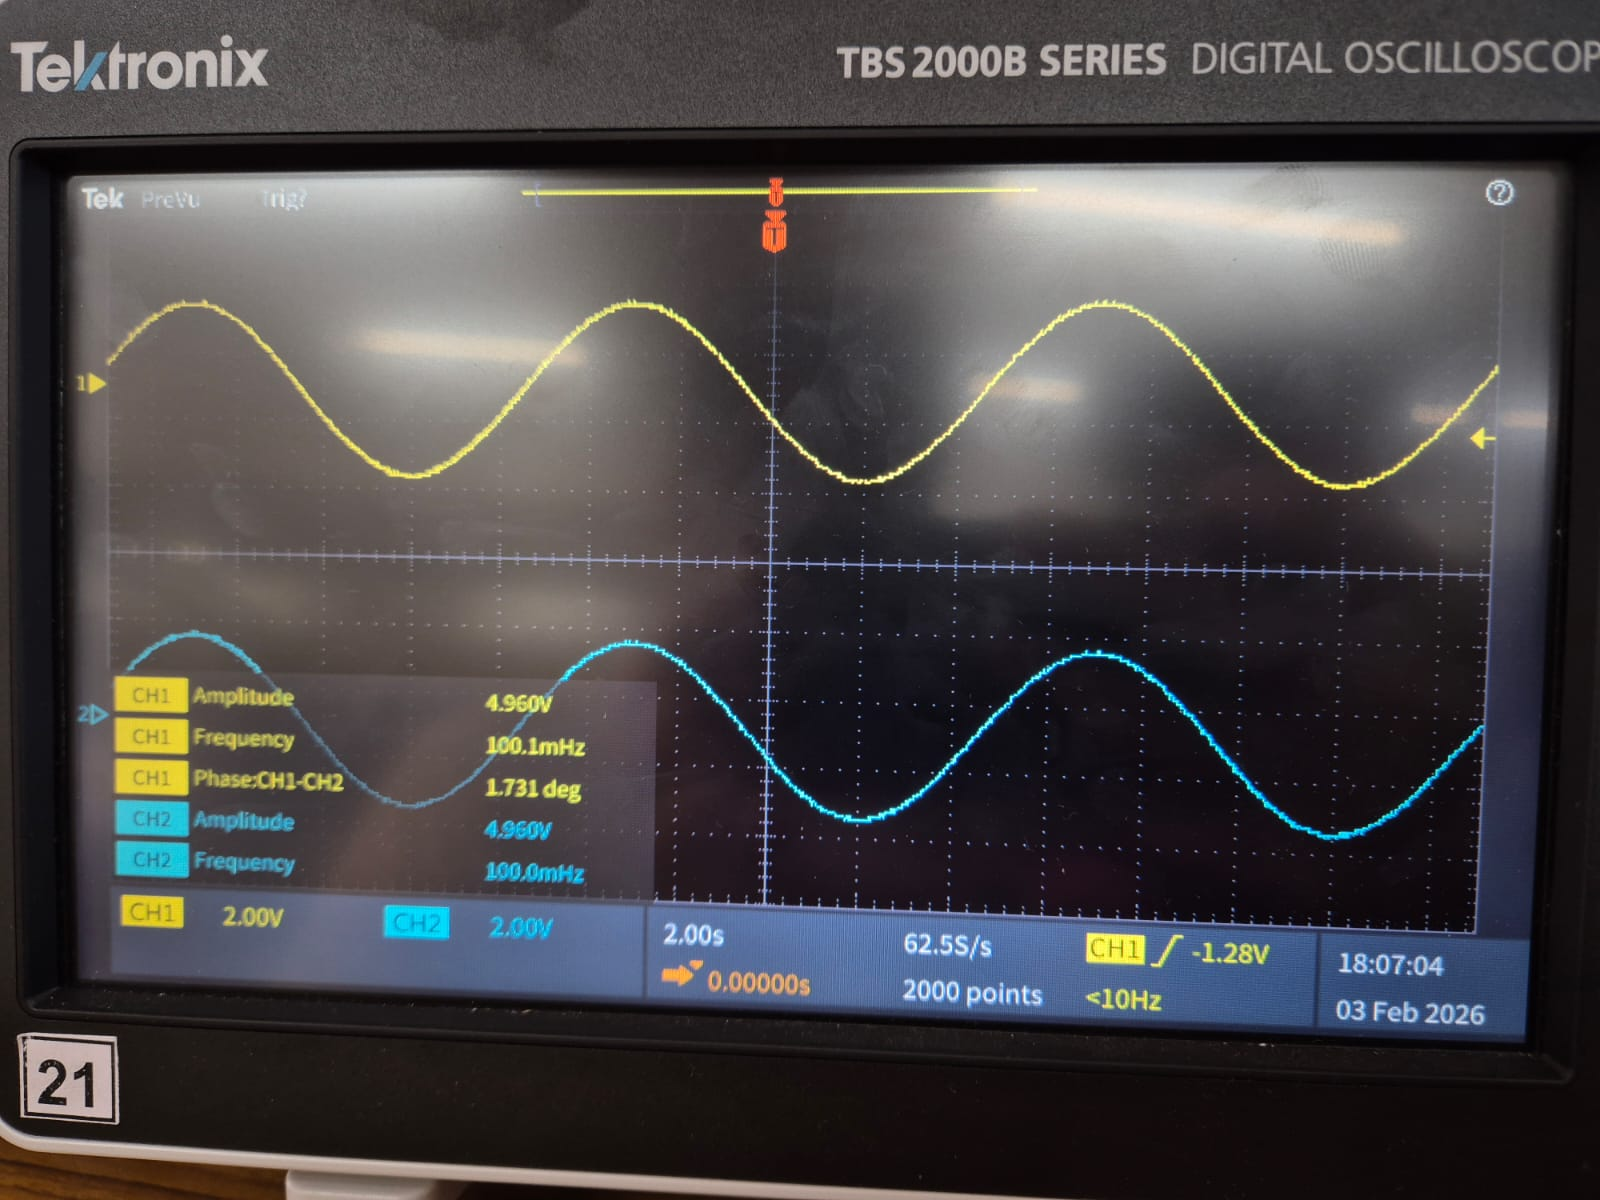
\includegraphics[width=\textwidth]{100mrc.jpeg}
    \caption*{(a) 100mHz}
    \end{subfigure}
%     \hfill
    \begin{subfigure}[b]{0.4\textwidth}
    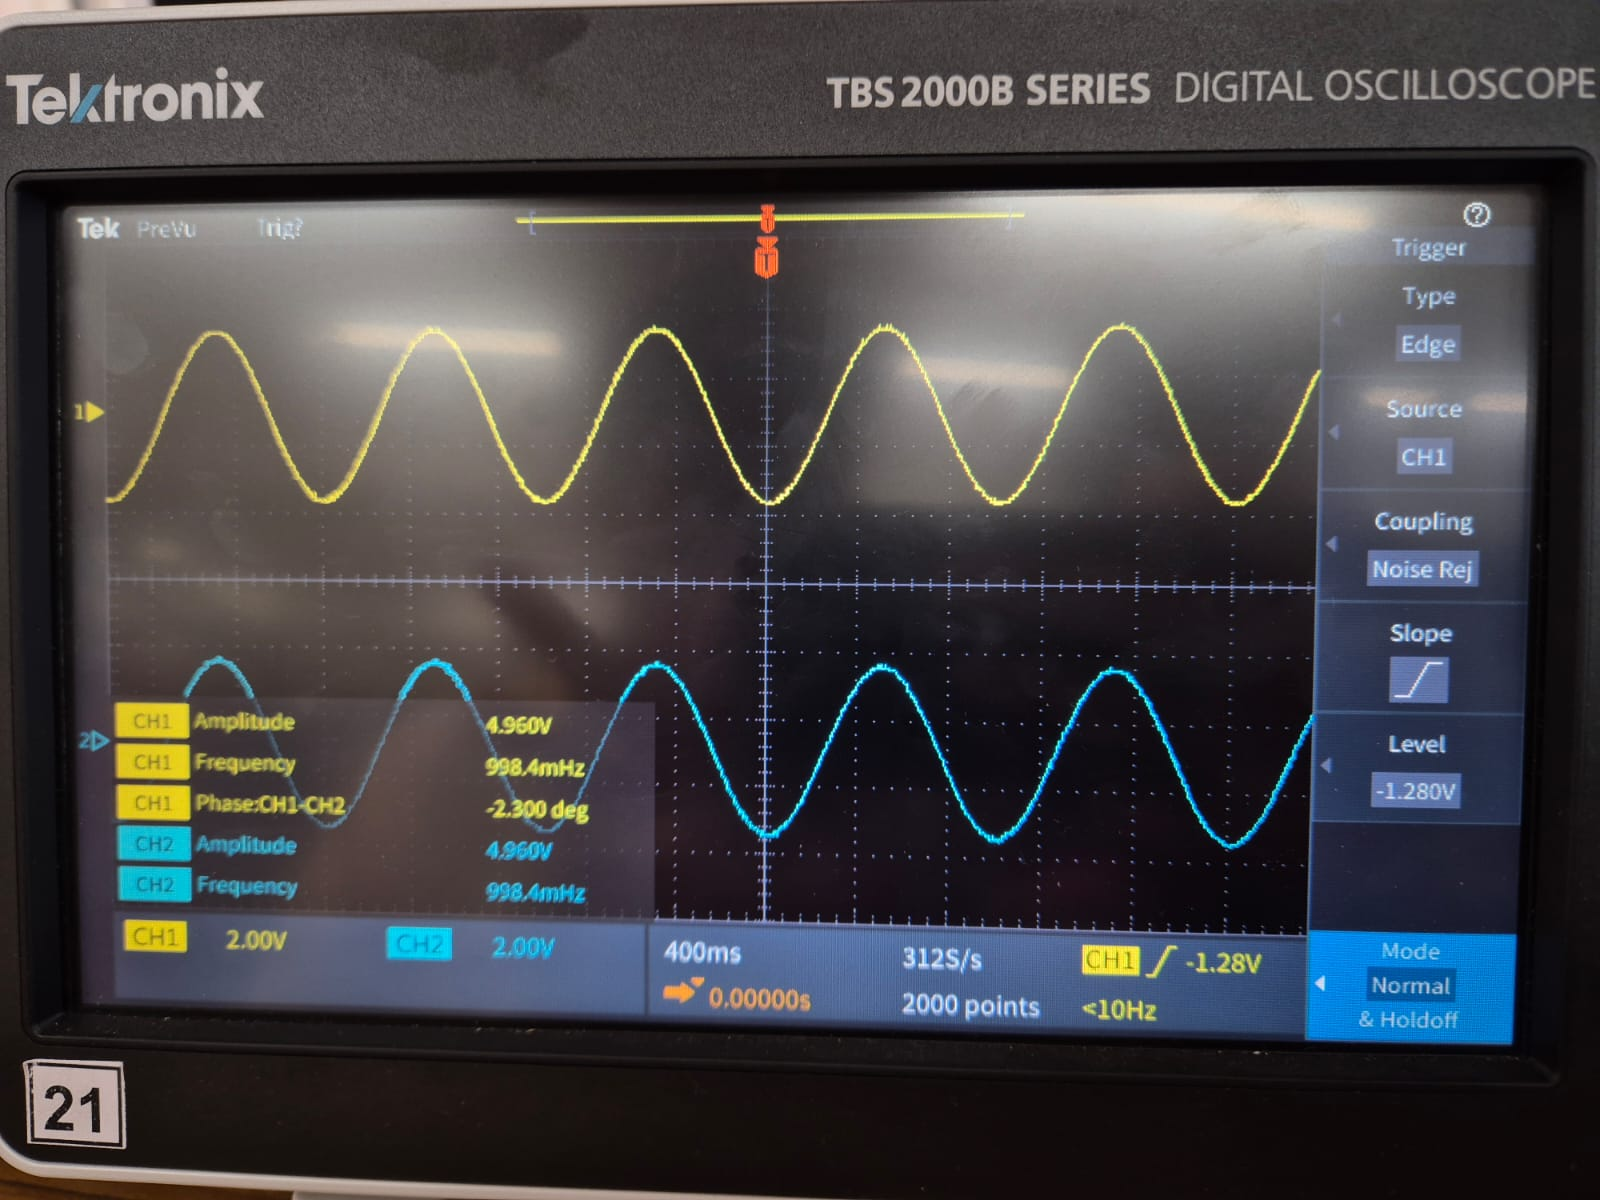
\includegraphics[width=\textwidth]{1rc.jpeg}
    \caption*{(b) 1Hz}
    \centering
    \end{subfigure}
\end{figure}
\vspace{10pt}
\begin{figure}[H]
     \centering
     \begin{subfigure}[b]{0.4\textwidth}
    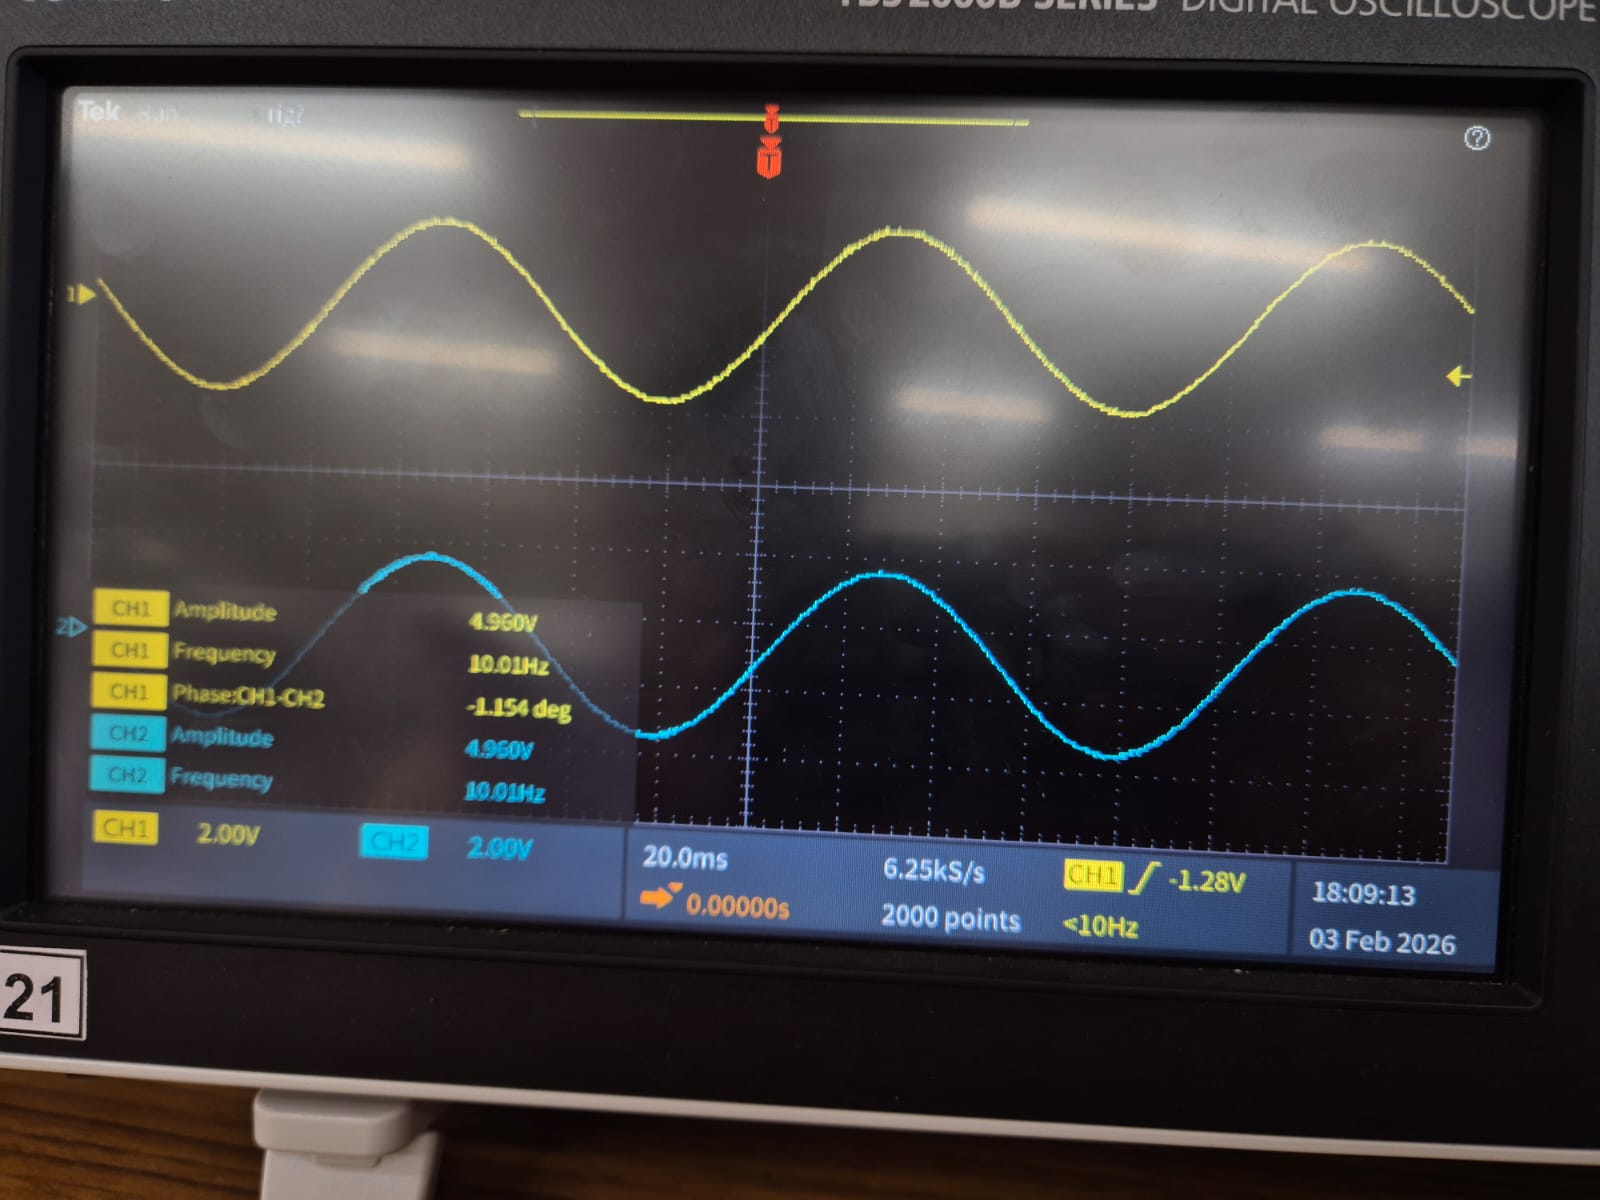
\includegraphics[width=\textwidth]{10rc.jpeg}
    \caption*{(c)10Hz}
    \centering
    \end{subfigure}
 \begin{subfigure}[b]{0.4\textwidth}
    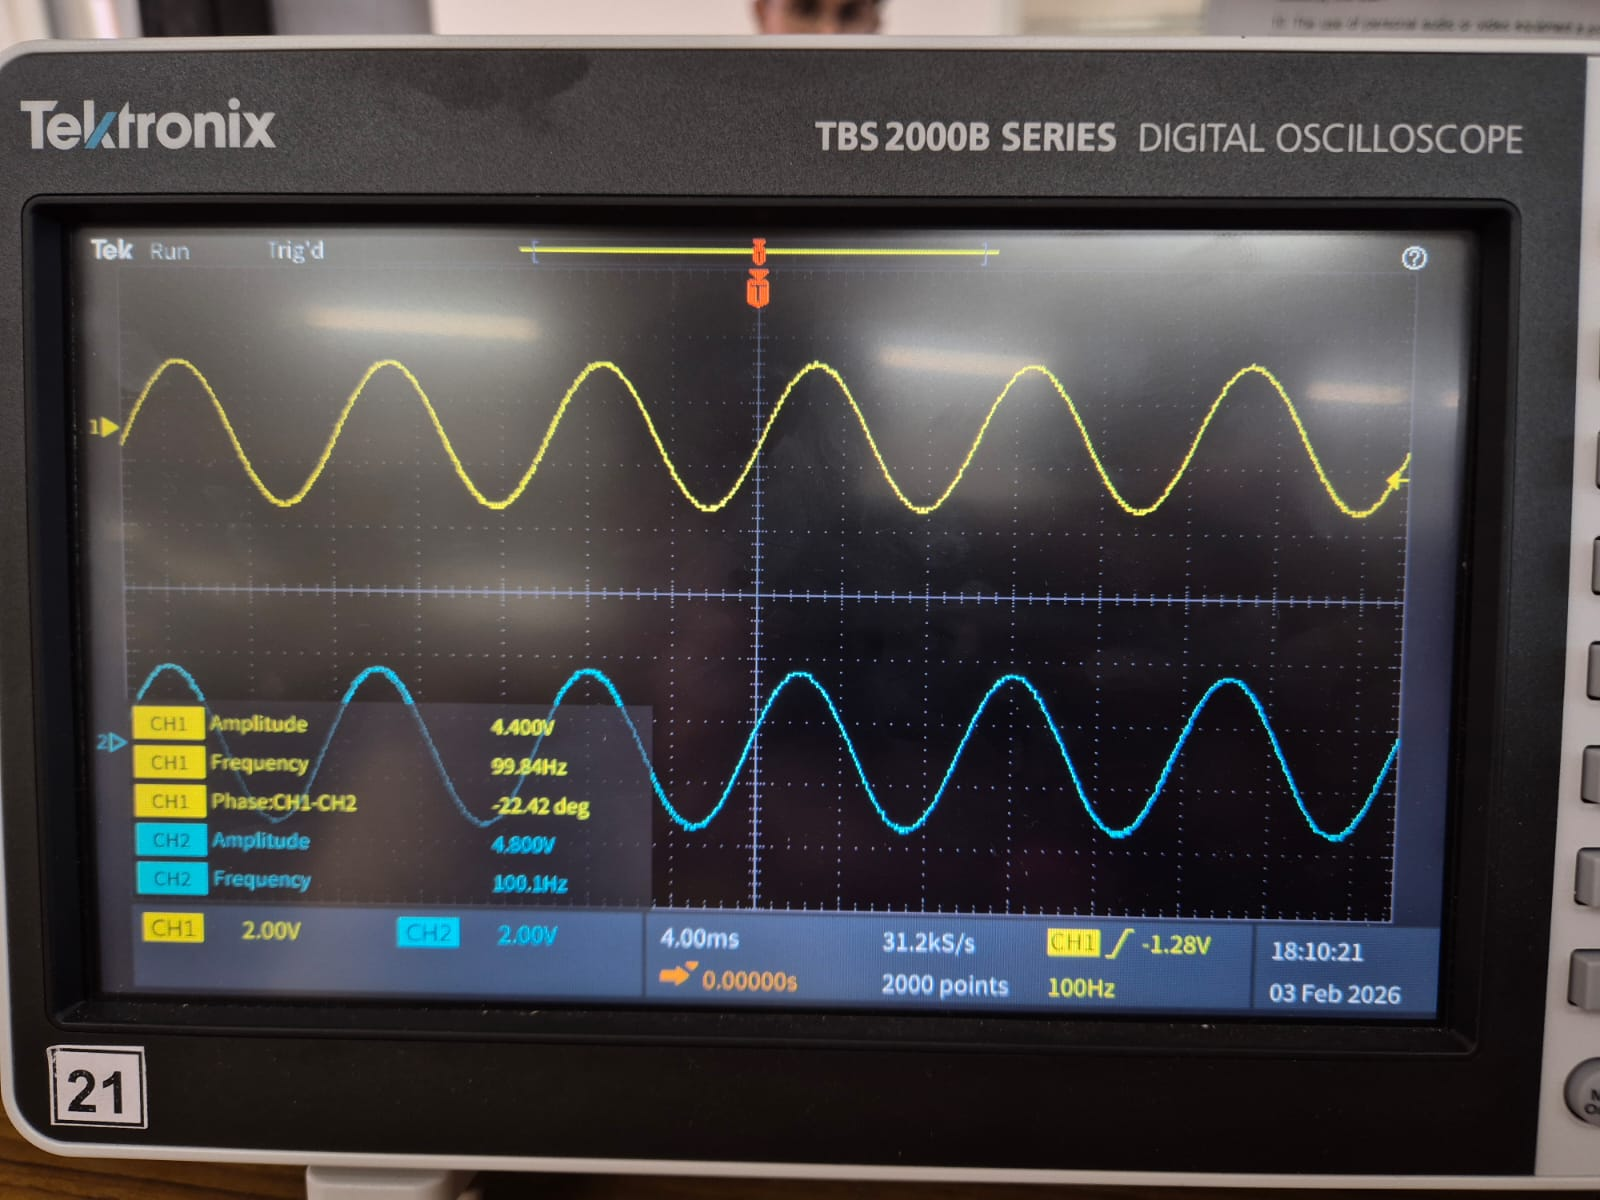
\includegraphics[width=\textwidth]{100rc.jpeg}
    \caption*{(d)100Hz}
    \centering
    \end{subfigure}
\end{figure}  
    \vspace{10pt}

\begin{figure}
\centering
     \begin{subfigure}[b]{0.4\textwidth}
    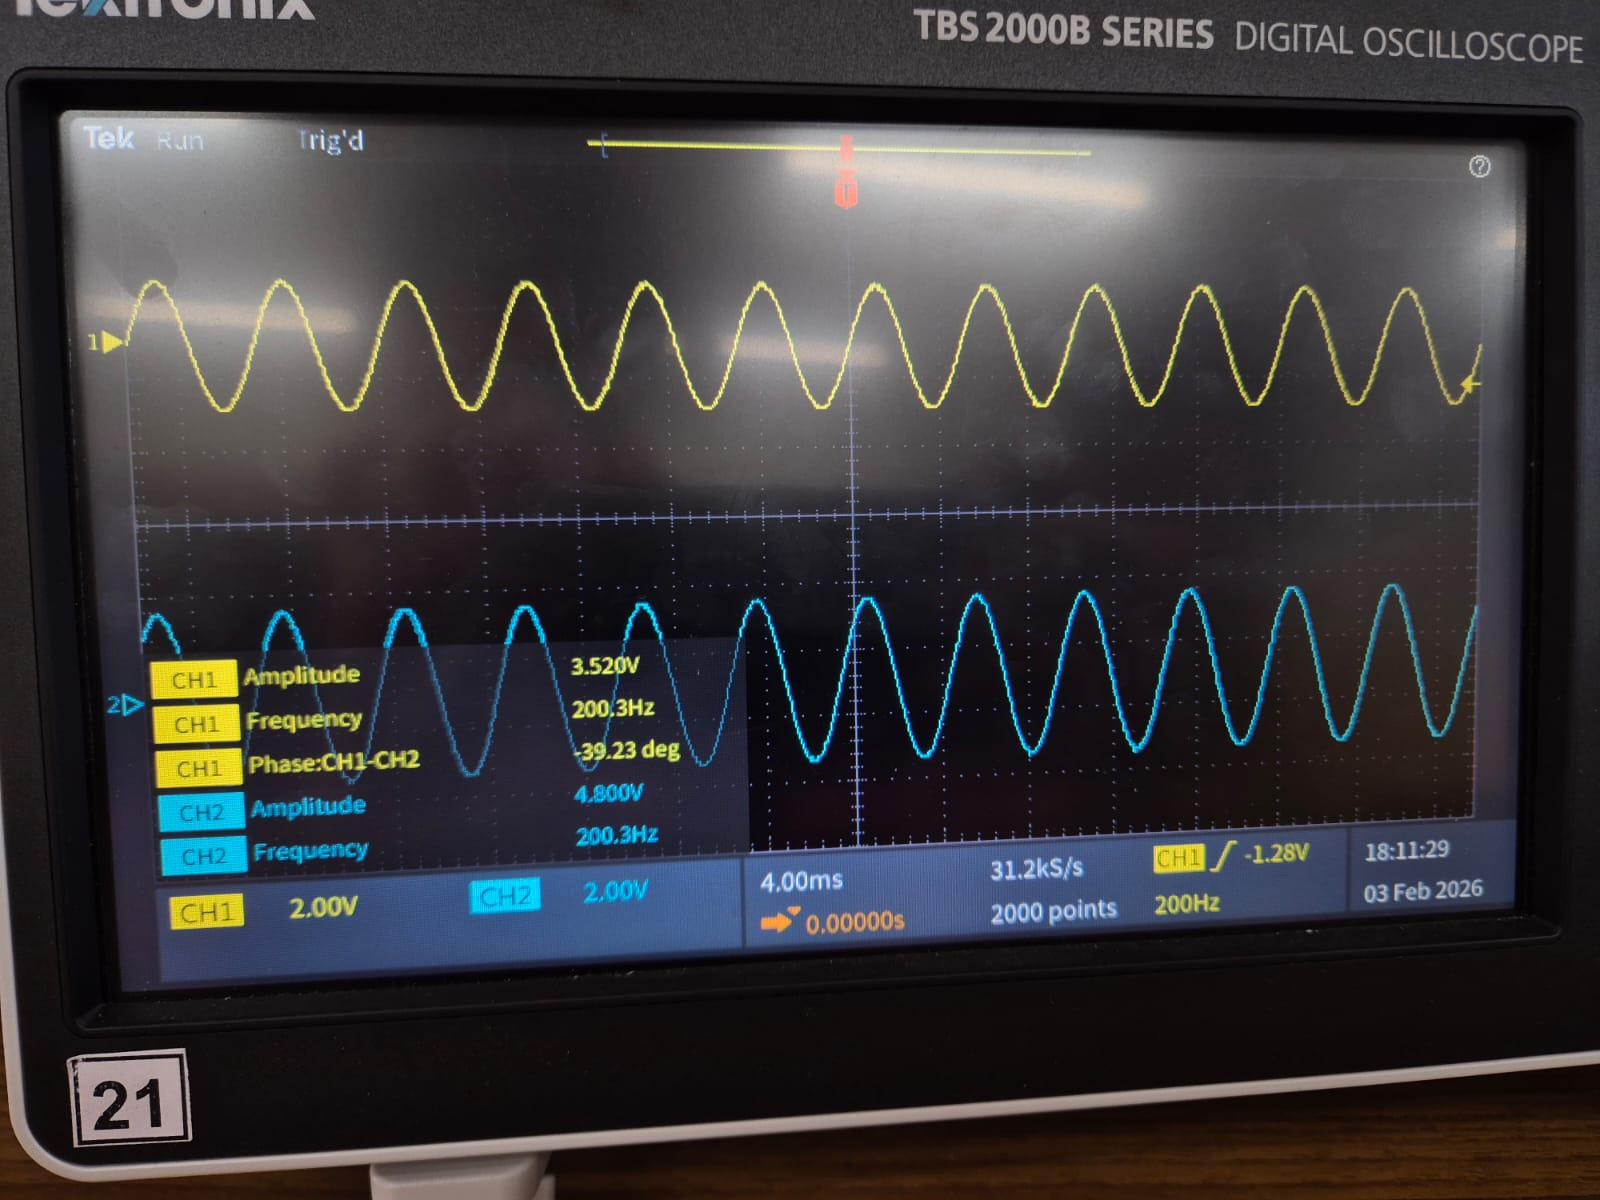
\includegraphics[width=\textwidth]{200rc.jpeg}
    \caption*{(e)200Hz}
    \end{subfigure}
     \begin{subfigure}[b]{0.4\textwidth}
    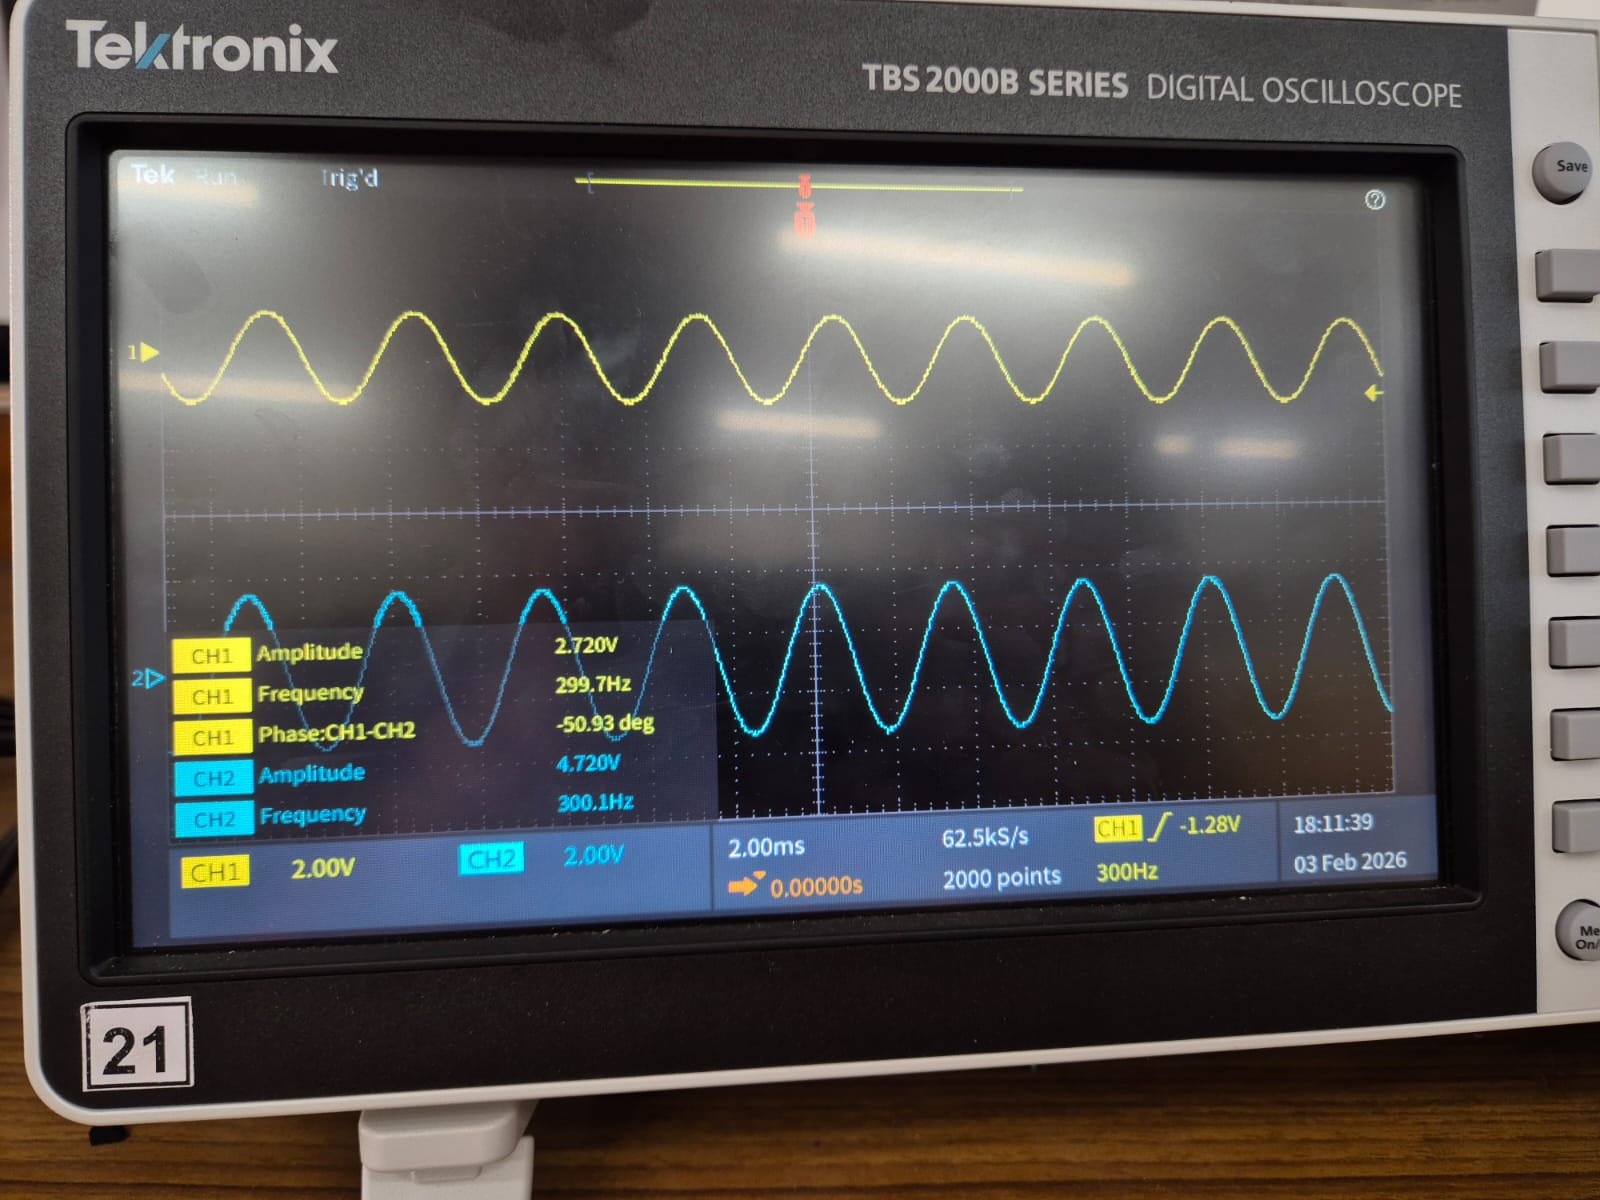
\includegraphics[width=\textwidth]{300rc.jpeg}
    \caption*{(f)300Hz}
    \end{subfigure}
\end{figure}
\vspace{10pt}
\begin{figure}
\centering
     \begin{subfigure}[b]{0.4\textwidth}
    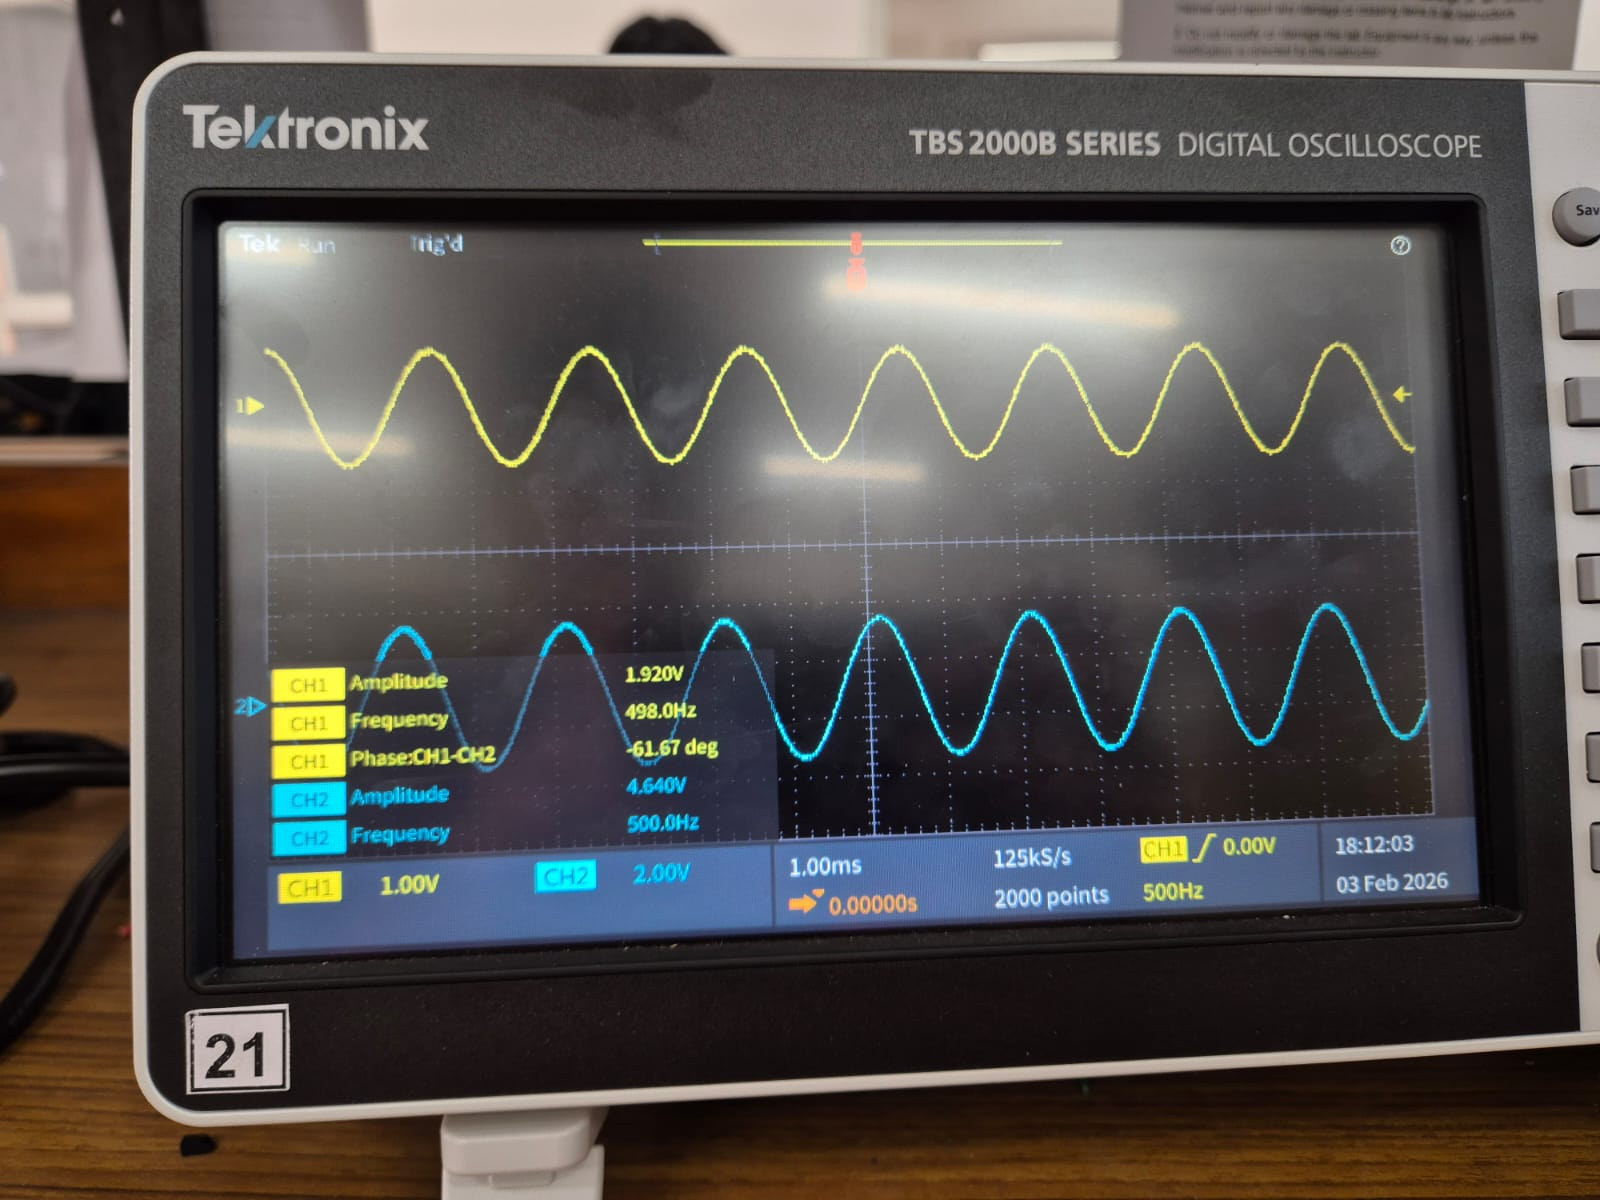
\includegraphics[width=\textwidth]{500rc.jpeg}
    \caption*{(g)500Hz}
    \end{subfigure}
    \begin{subfigure}[b]{0.4\textwidth}
    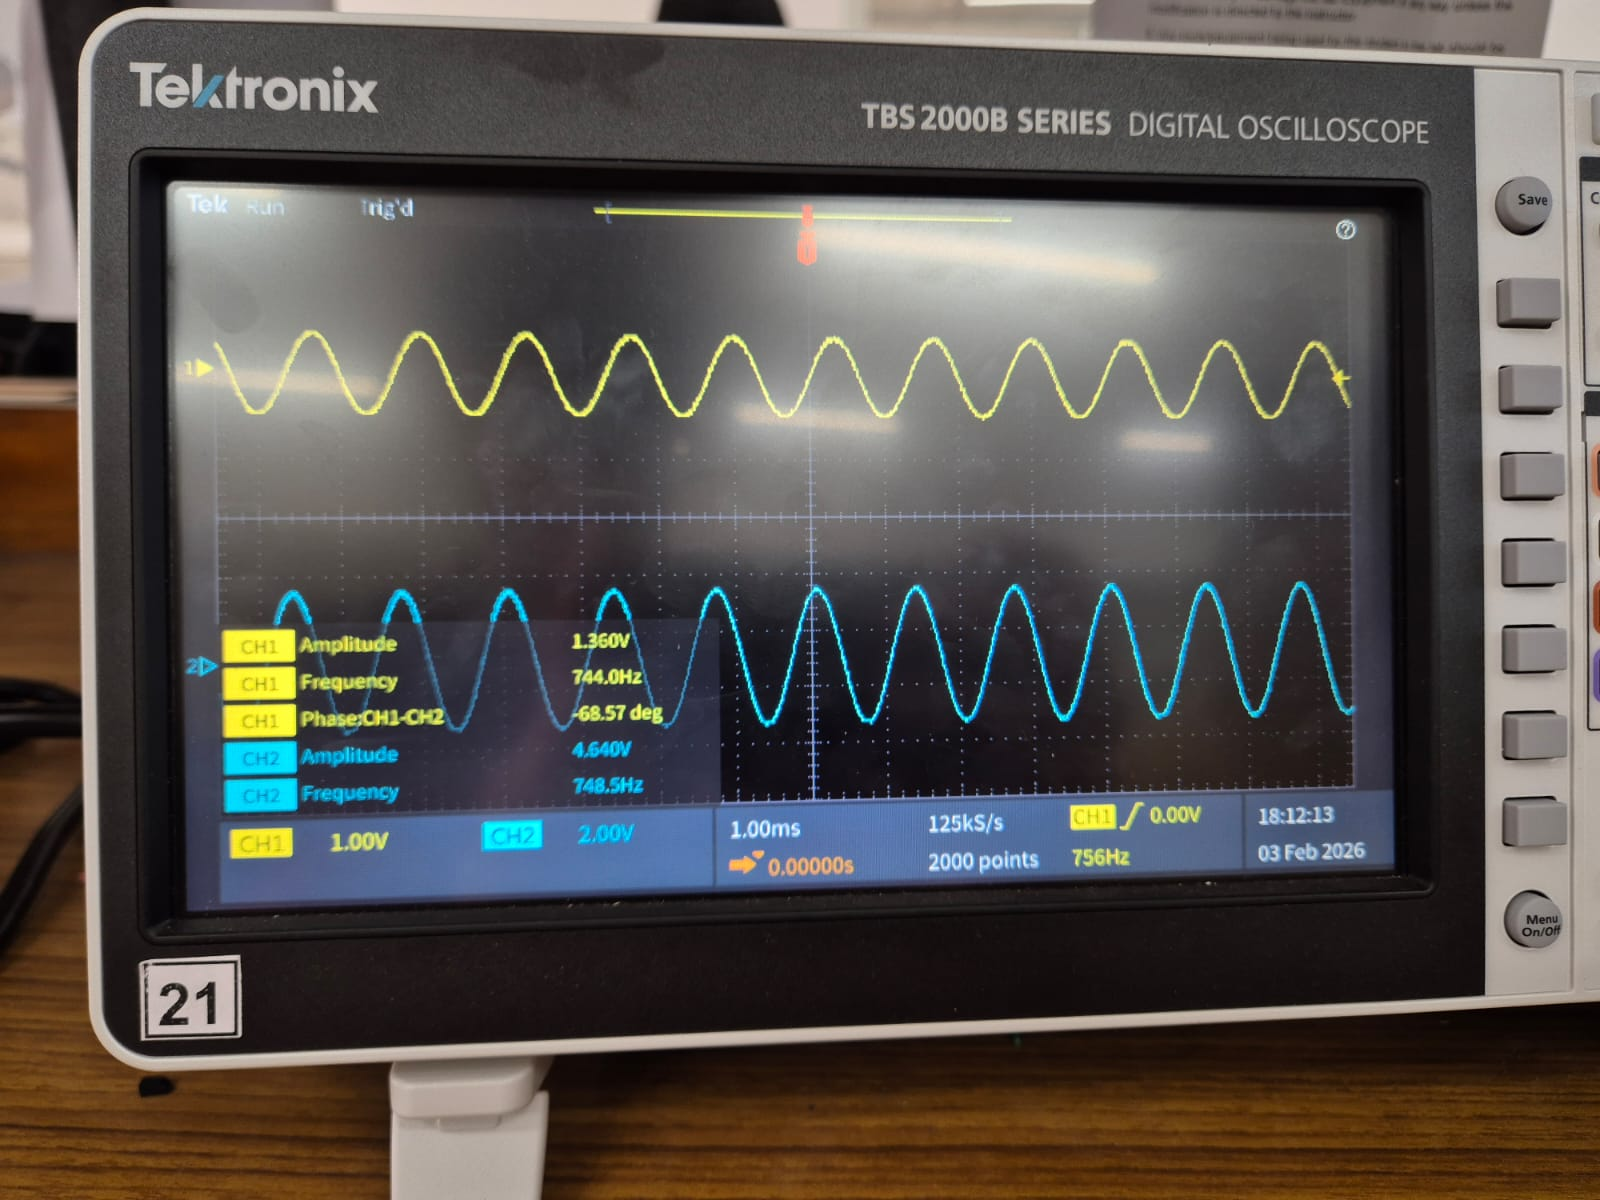
\includegraphics[width=\textwidth]{750rc.jpeg}
    \caption*{(h)750Hz}
    \end{subfigure}
\end{figure}
\vspace{10pt}
\begin{figure}[H]
\centering
     \begin{subfigure}[b]{0.4\textwidth}
    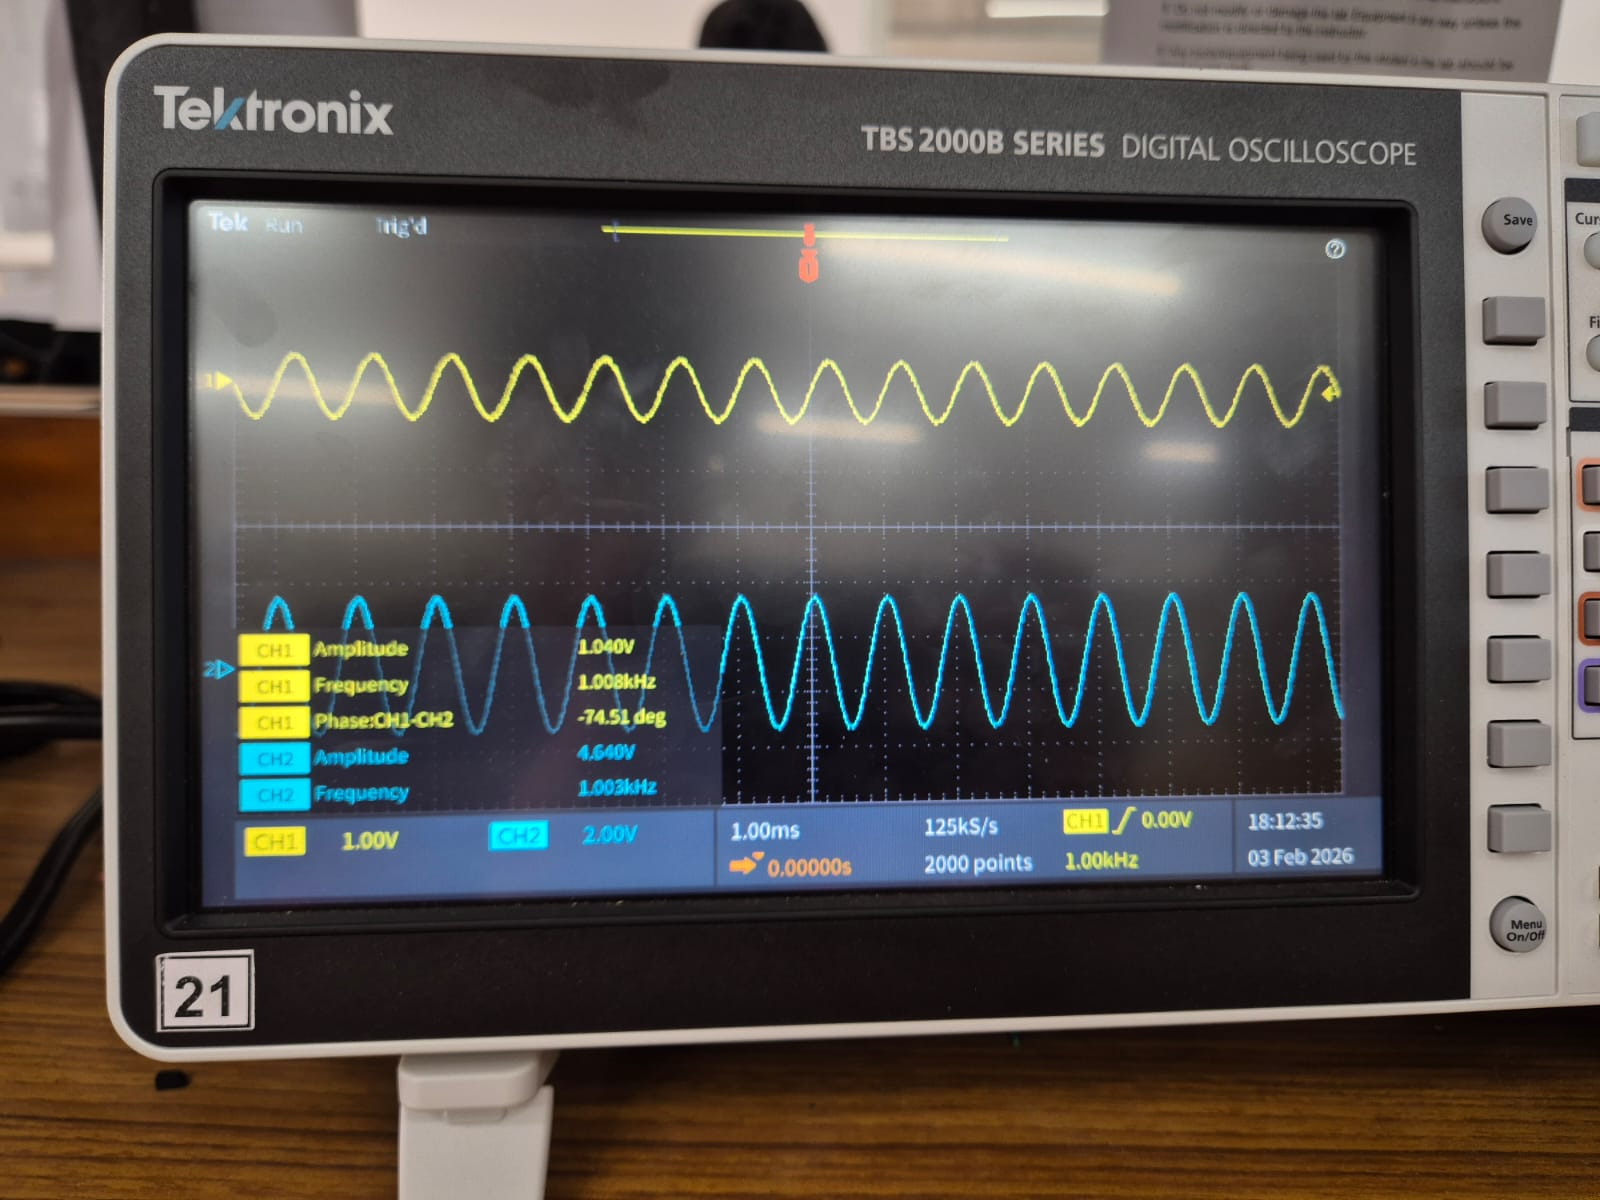
\includegraphics[width=\textwidth]{1krc.jpeg}
        \caption*{(i)1kHz}
    \end{subfigure}
     \begin{subfigure}[b]{0.4\textwidth}
    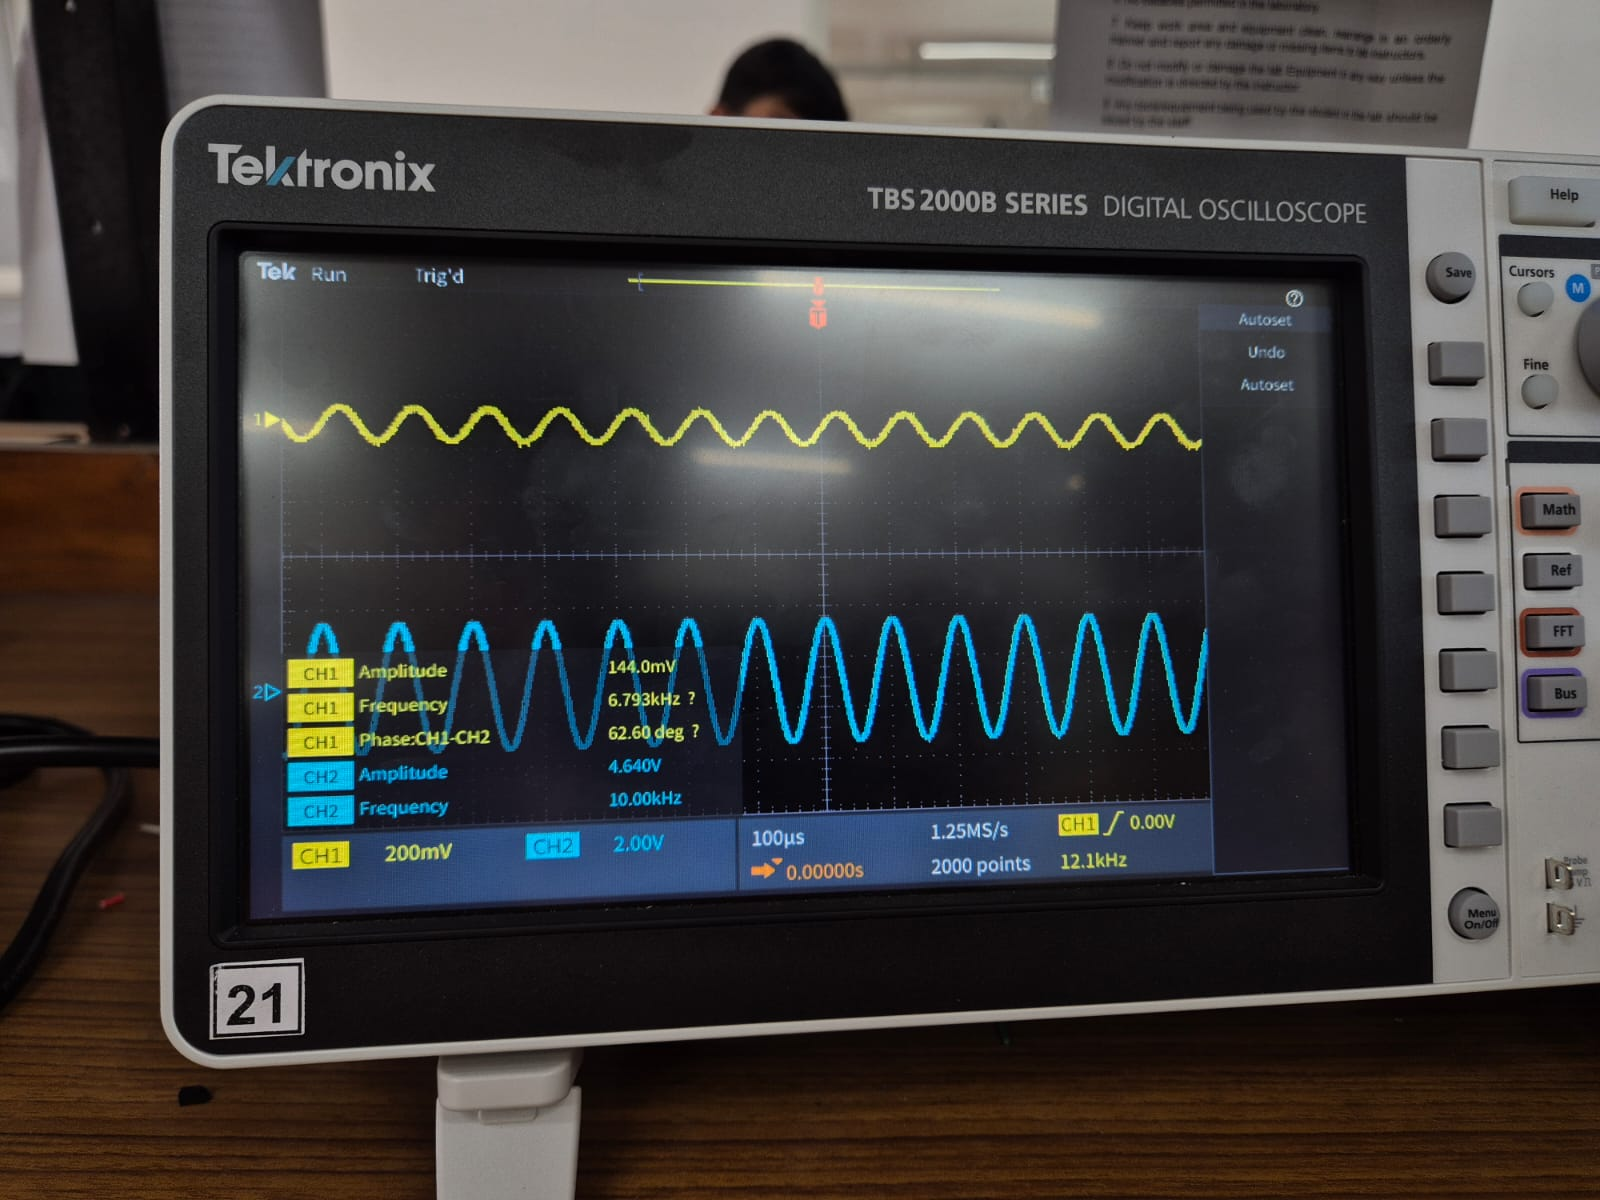
\includegraphics[width=\textwidth]{10krc.jpeg}
        \caption*{(j)10kHz}
    \end{subfigure}
\end{figure}
\vspace{10pt}
\begin{figure}[H]
\centering
     \begin{subfigure}[h]{0.4\textwidth}
    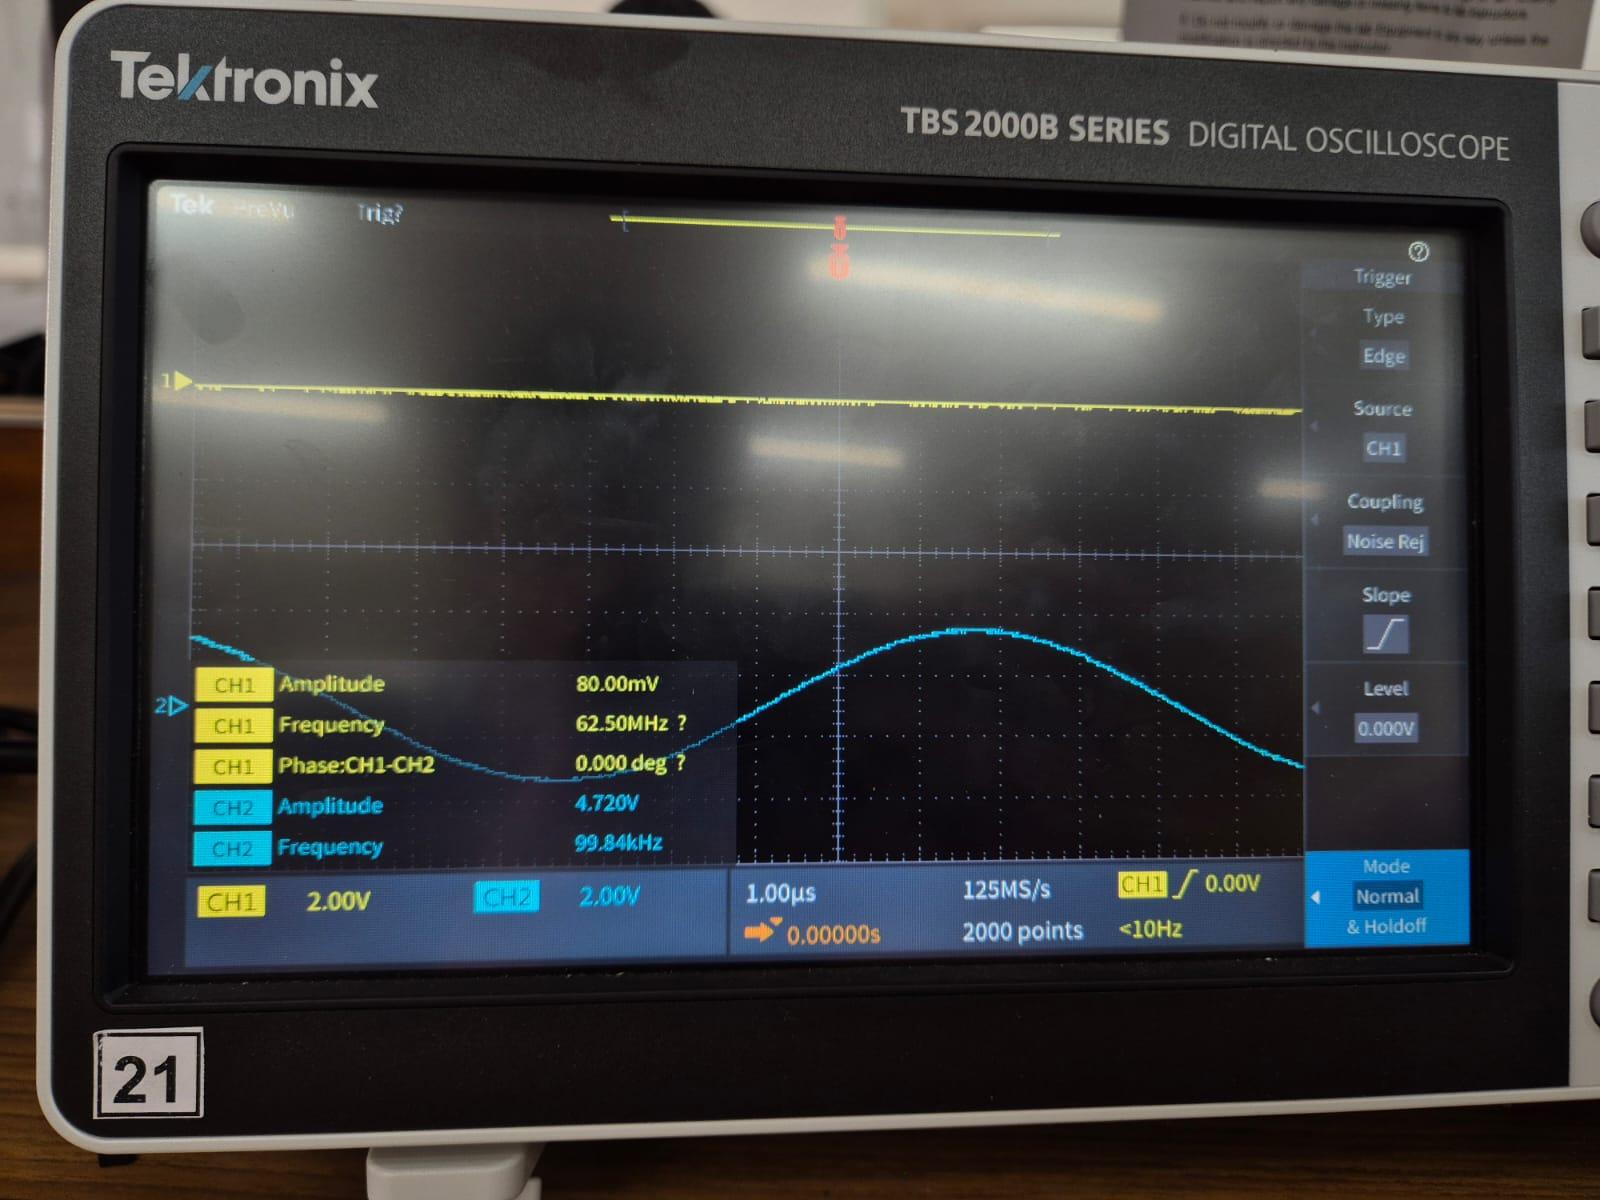
\includegraphics[width=\textwidth]{100krc.jpeg}
        \caption*{(k)100kHz}
    \end{subfigure}
     \begin{subfigure}[h]{0.4\textwidth}
    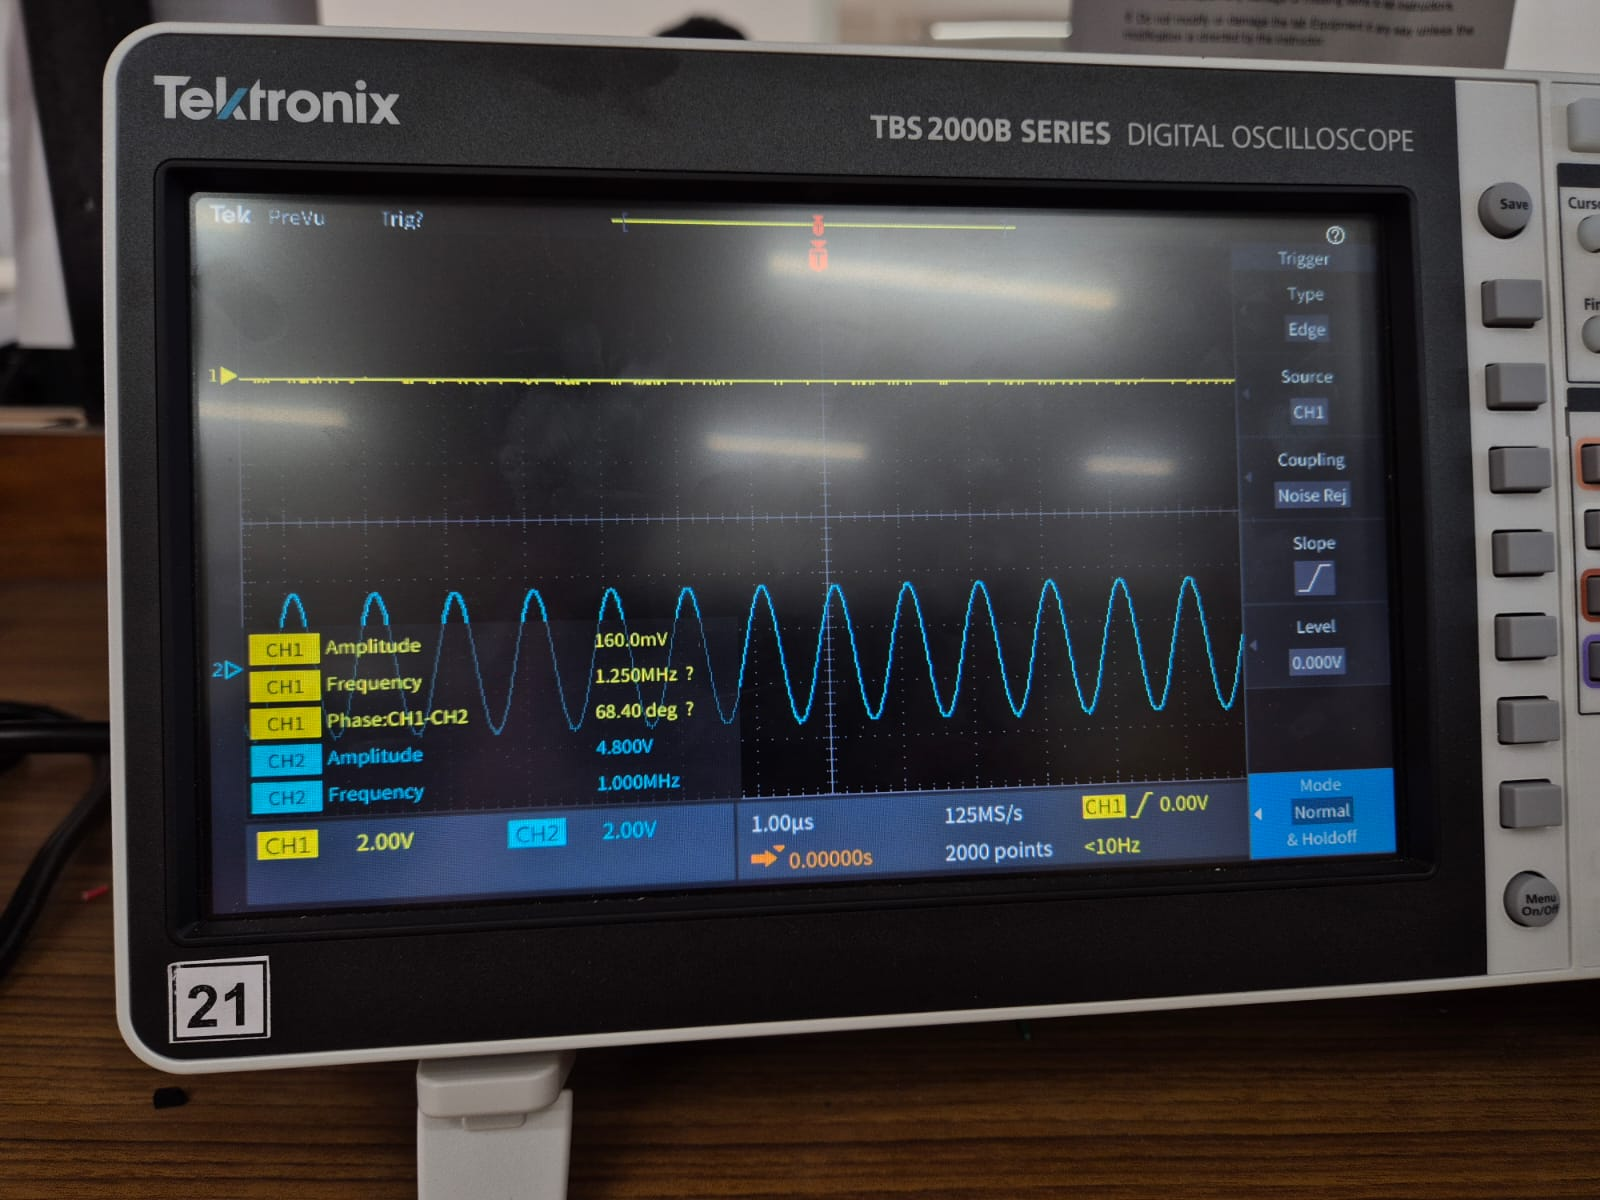
\includegraphics[width=\textwidth]{1Mrc.jpeg}
        \caption*{(l)1MHz}
    \end{subfigure}
    
\end{figure}
\subsection{Simulated Bode Plot}
\begin{figure}[H]
    \centering
    \begin{subfigure}[h]{0.4\textwidth}
    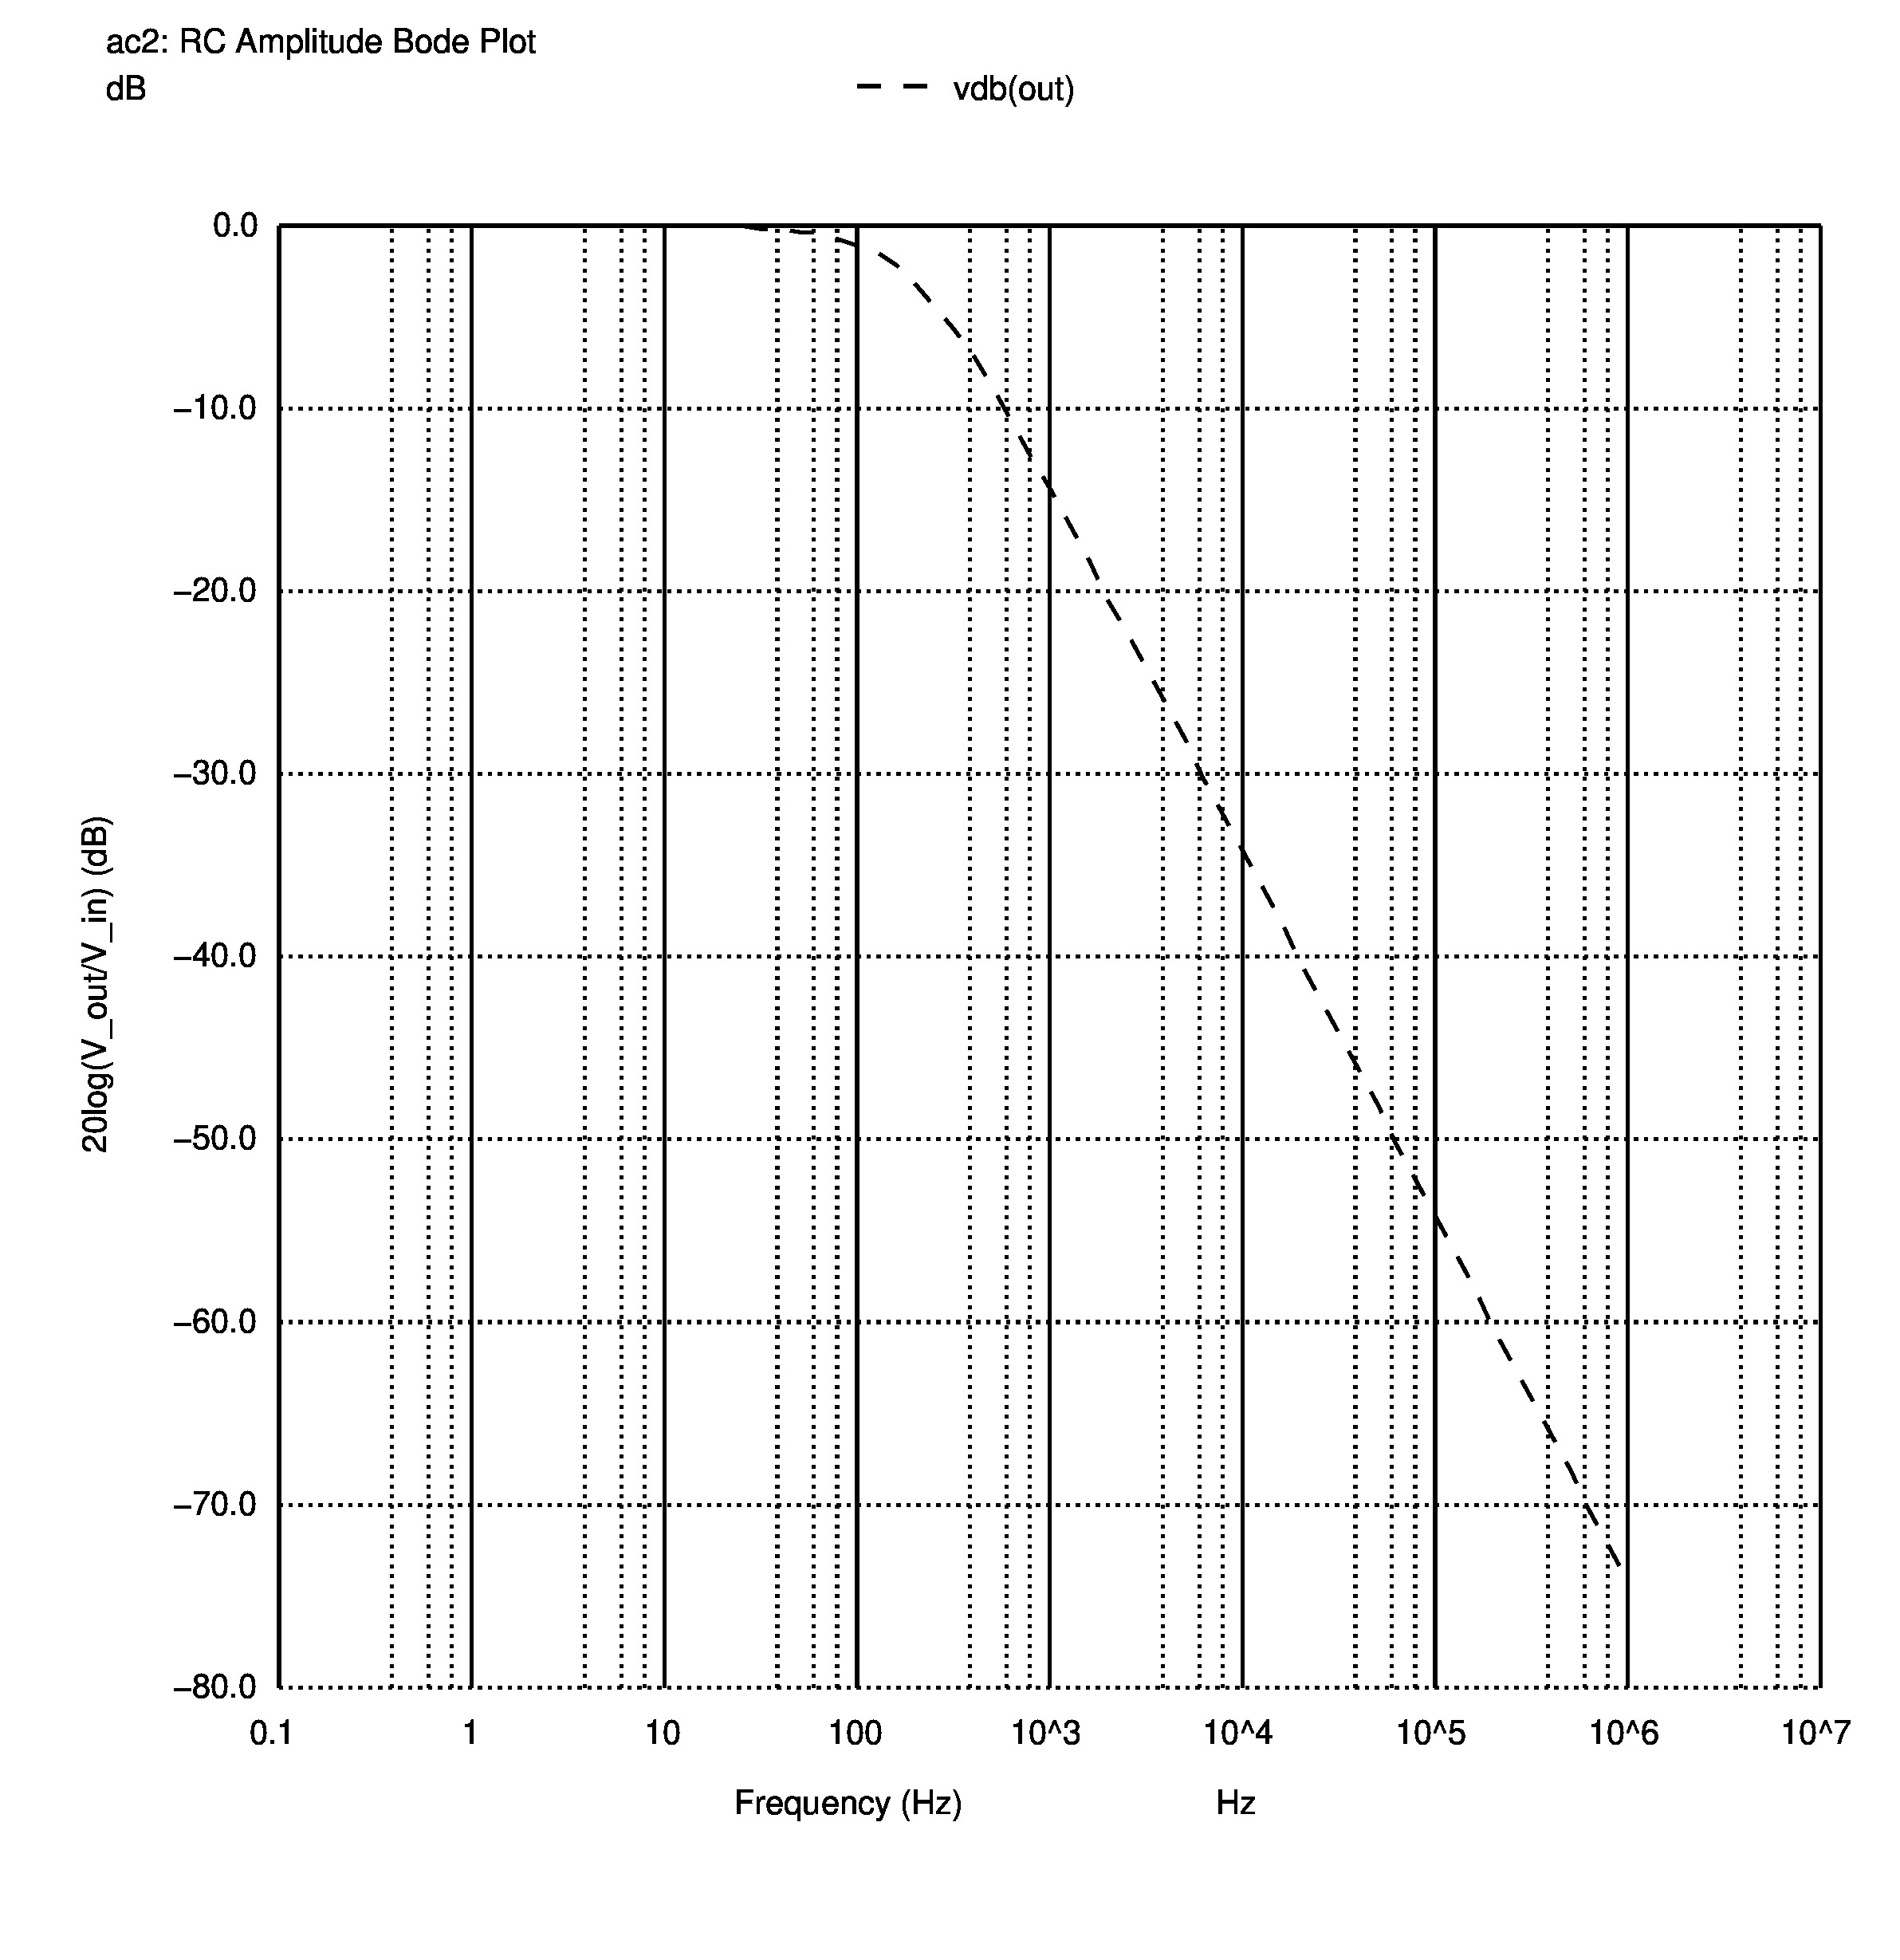
\includegraphics[width=\textwidth]{rc_amp.jpg}
    \caption{Amplitude Bode Plot}
\end{subfigure}
\begin{subfigure}[h]{0.4\textwidth}
    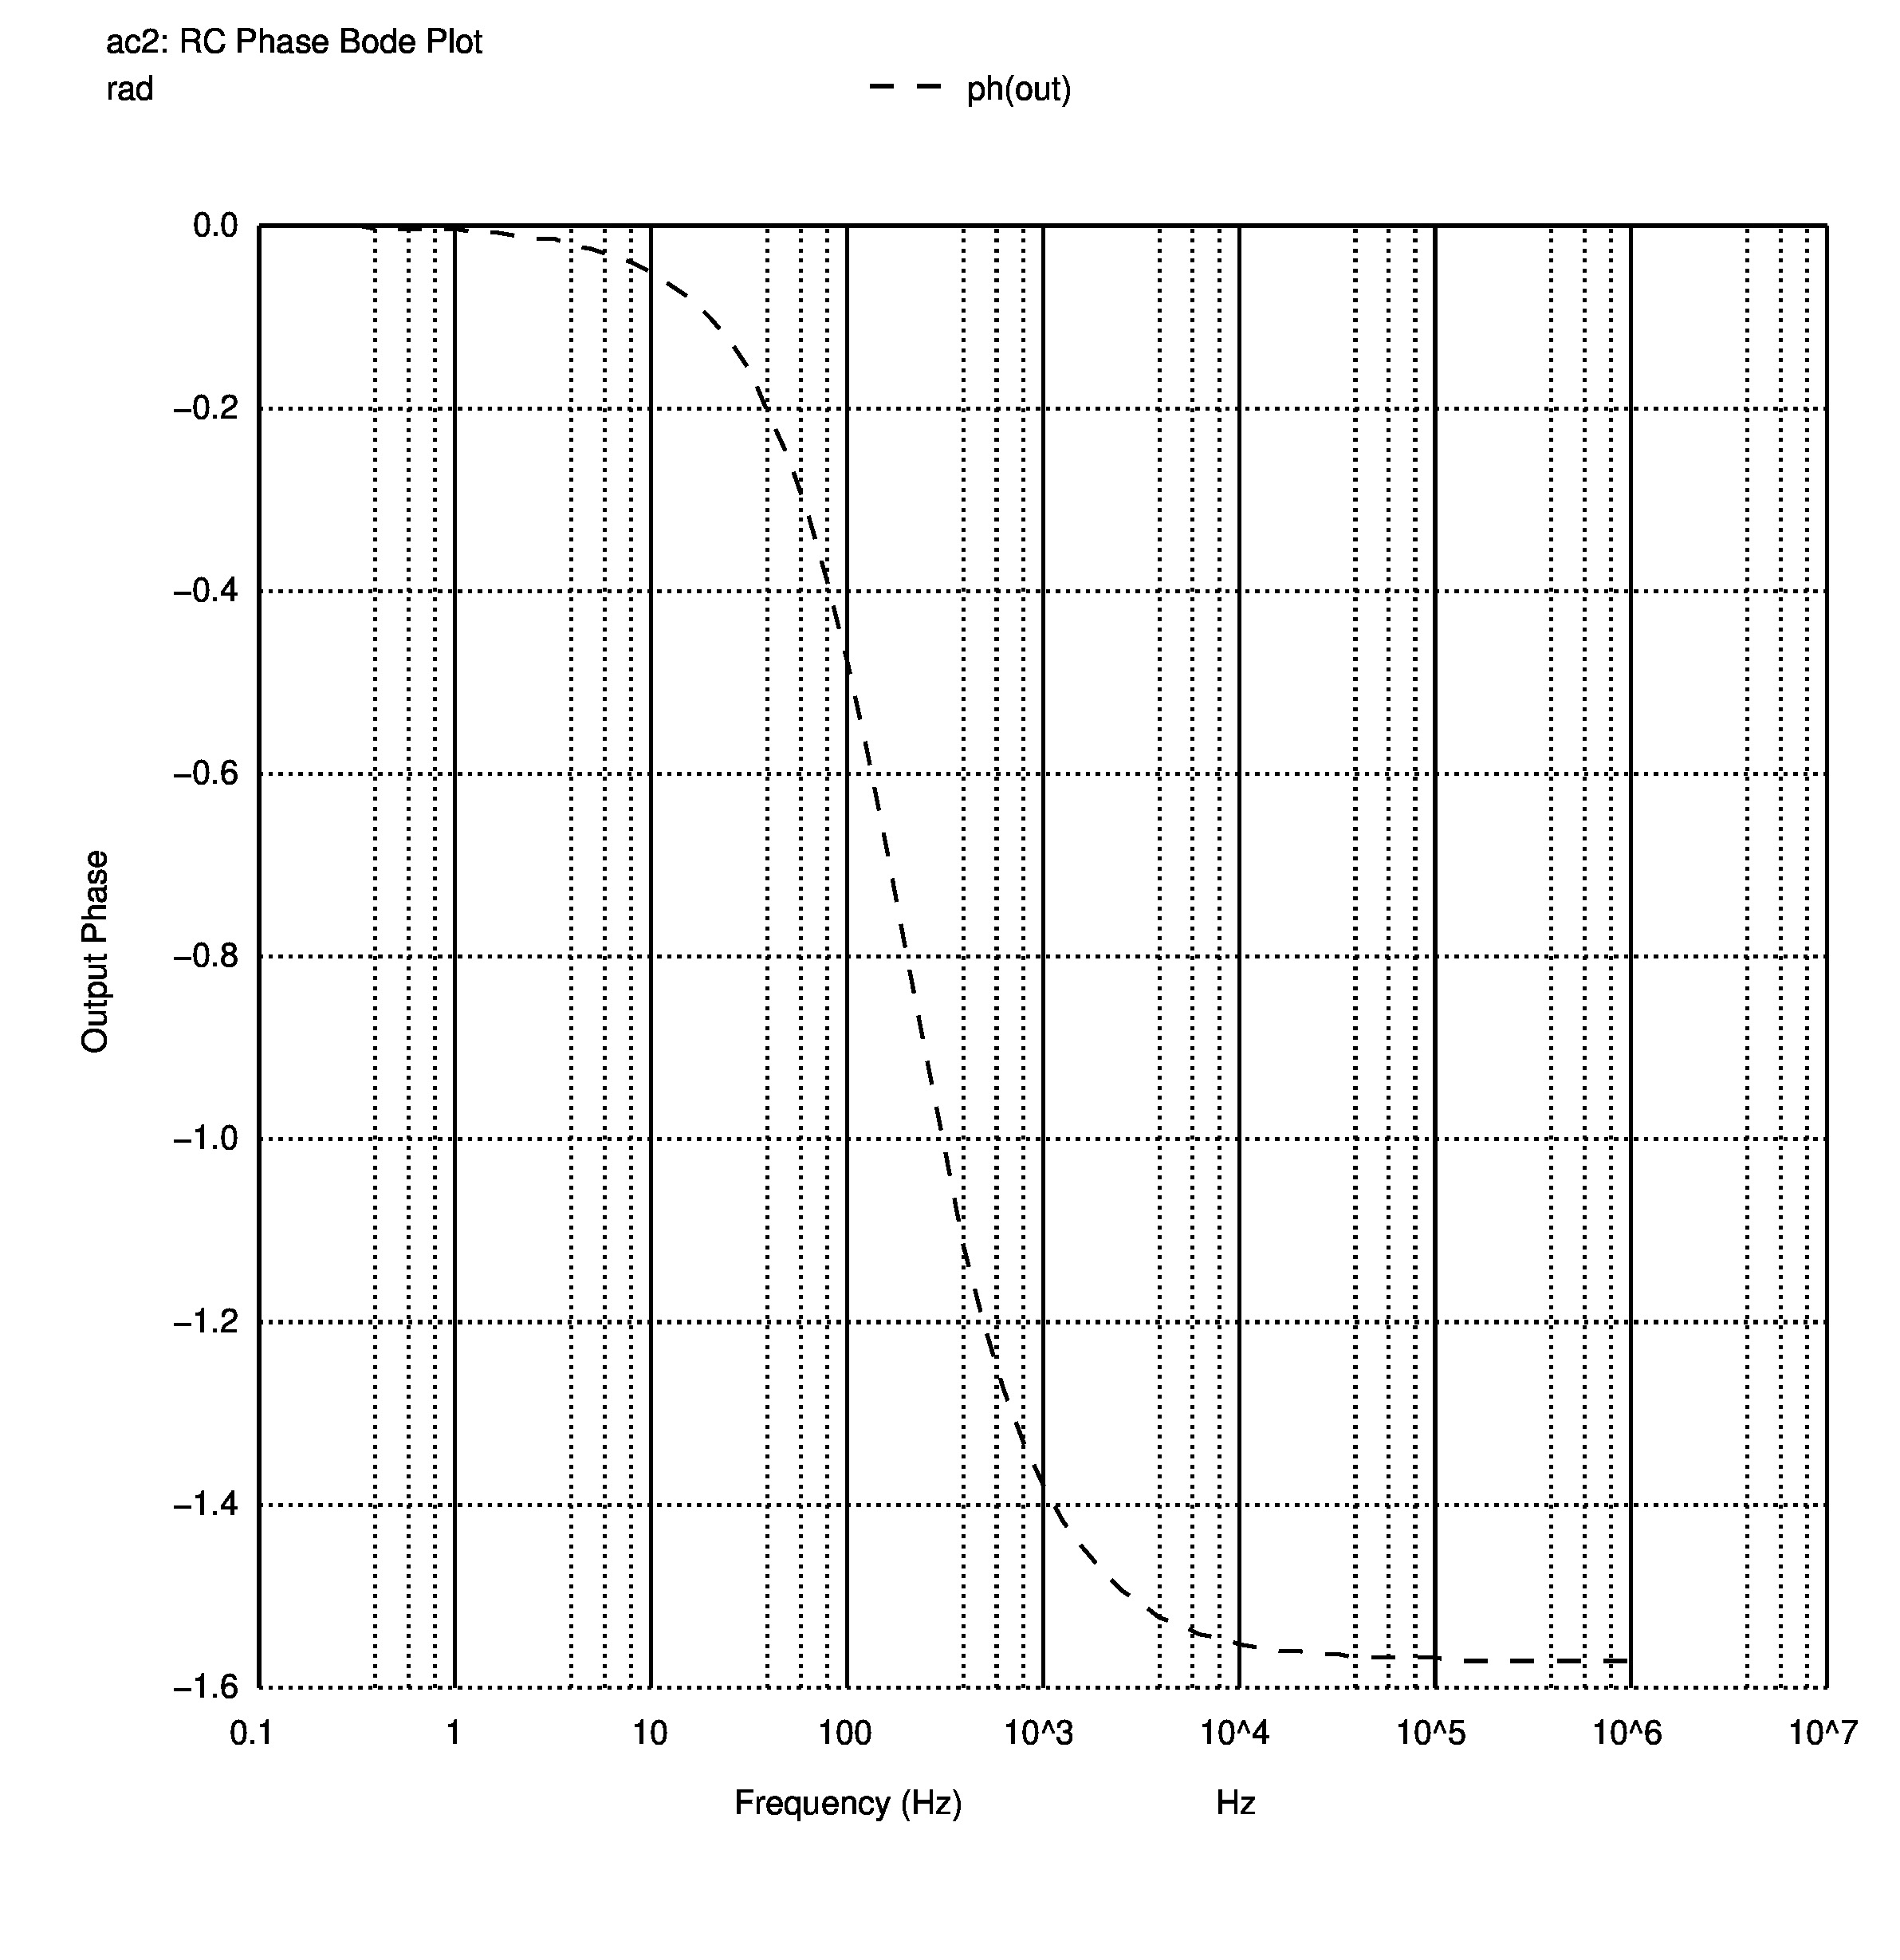
\includegraphics[width=\textwidth]{rc_ph.jpg}
    \caption{Phase Bode Plot}
\end{subfigure}
\end{figure}
\subsection{Manual Bode Plot}
\begin{figure}[H]
    \centering
\begin{subfigure}[h]{0.4\textwidth}
    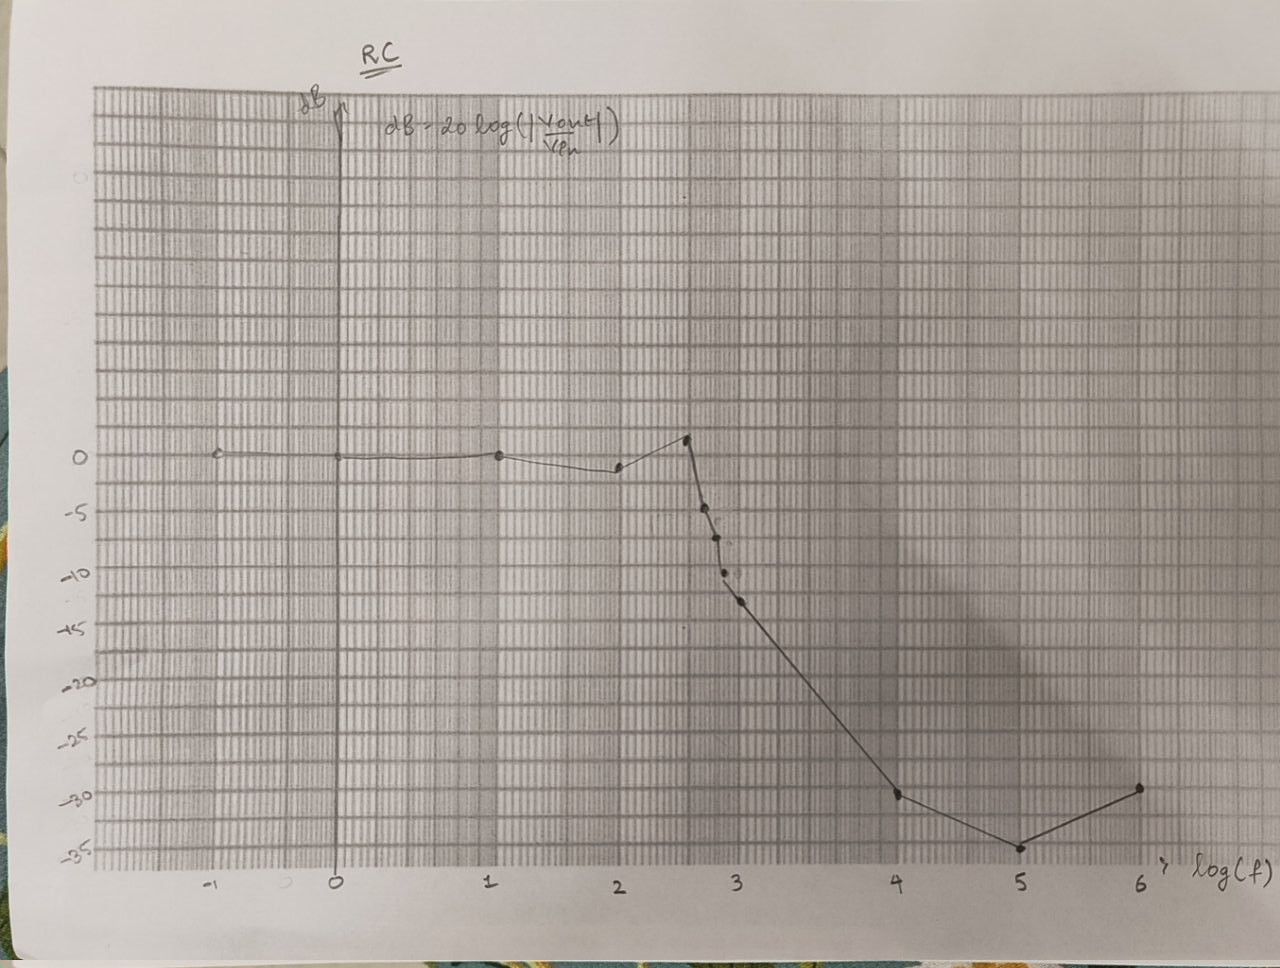
\includegraphics[width=\textwidth]{amp1.jpeg}
    \caption{Amplitude Bode Plot}
\end{subfigure}
\end{figure}
%kaedbfjldfbzv

\subsection{Results}
\begin{table}[H]
    \centering
    \begin{tabular}{cccc}
        \toprule
        Frequency & Measured $\frac{V_{out}}{V_{in}}$ \\
        \midrule
         $100mHz$ & $1$ \\
        $1Hz$ & $1$ \\
        $10Hz$ & $1$ \\
         $100Hz$ & $0.917$ \\
         $200Hz$ & $1.257$ \\
         $300Hz$ & $0.576$ \\
         $500Hz$ & $0.414$ \\
         $750Hz$ & $0.293$ \\
         $1kHz$ & $0.224$ \\
         $10kHz$ & $0.031$ \\
         $100kHz$ & $0.017$ \\
         $1MHz$ & $0.033$ \\
        \bottomrule
    \end{tabular}
    \caption{Frequency Response for RC}
\end{table}
Thus, we see that the cutoff frequency $\left(=1/2\pi RC\right)$ is 194.1 Hz and the slope is roughly -20dB/decade.


\section{Part E: Frequency Response of CR circuit (High-Pass Filter)}
In this experiment we a apply a sinusoidal input with constant amplitude of $5V$ with varying frequency to a CR circuit and measure the output amplitude.\\
The goal is to identify the cut-off frequency and the slope of the Bode Plot.\\
\subsection{Theory}
Using Kirchoff's voltage law:
\begin{align}
    V=v_c+v_r \\
    V=iX_c+iR  \\
    V=i(\frac{1}{j\omega c}+R) \\
    v_r=iR=\frac{V}{1+\frac{1}{j\omega cR}}\\
\end{align}
\subsection{Measured Waveforms}
\begin{figure}[H]
    \centering
    \begin{subfigure}[b]{0.4\textwidth}
    \centering
    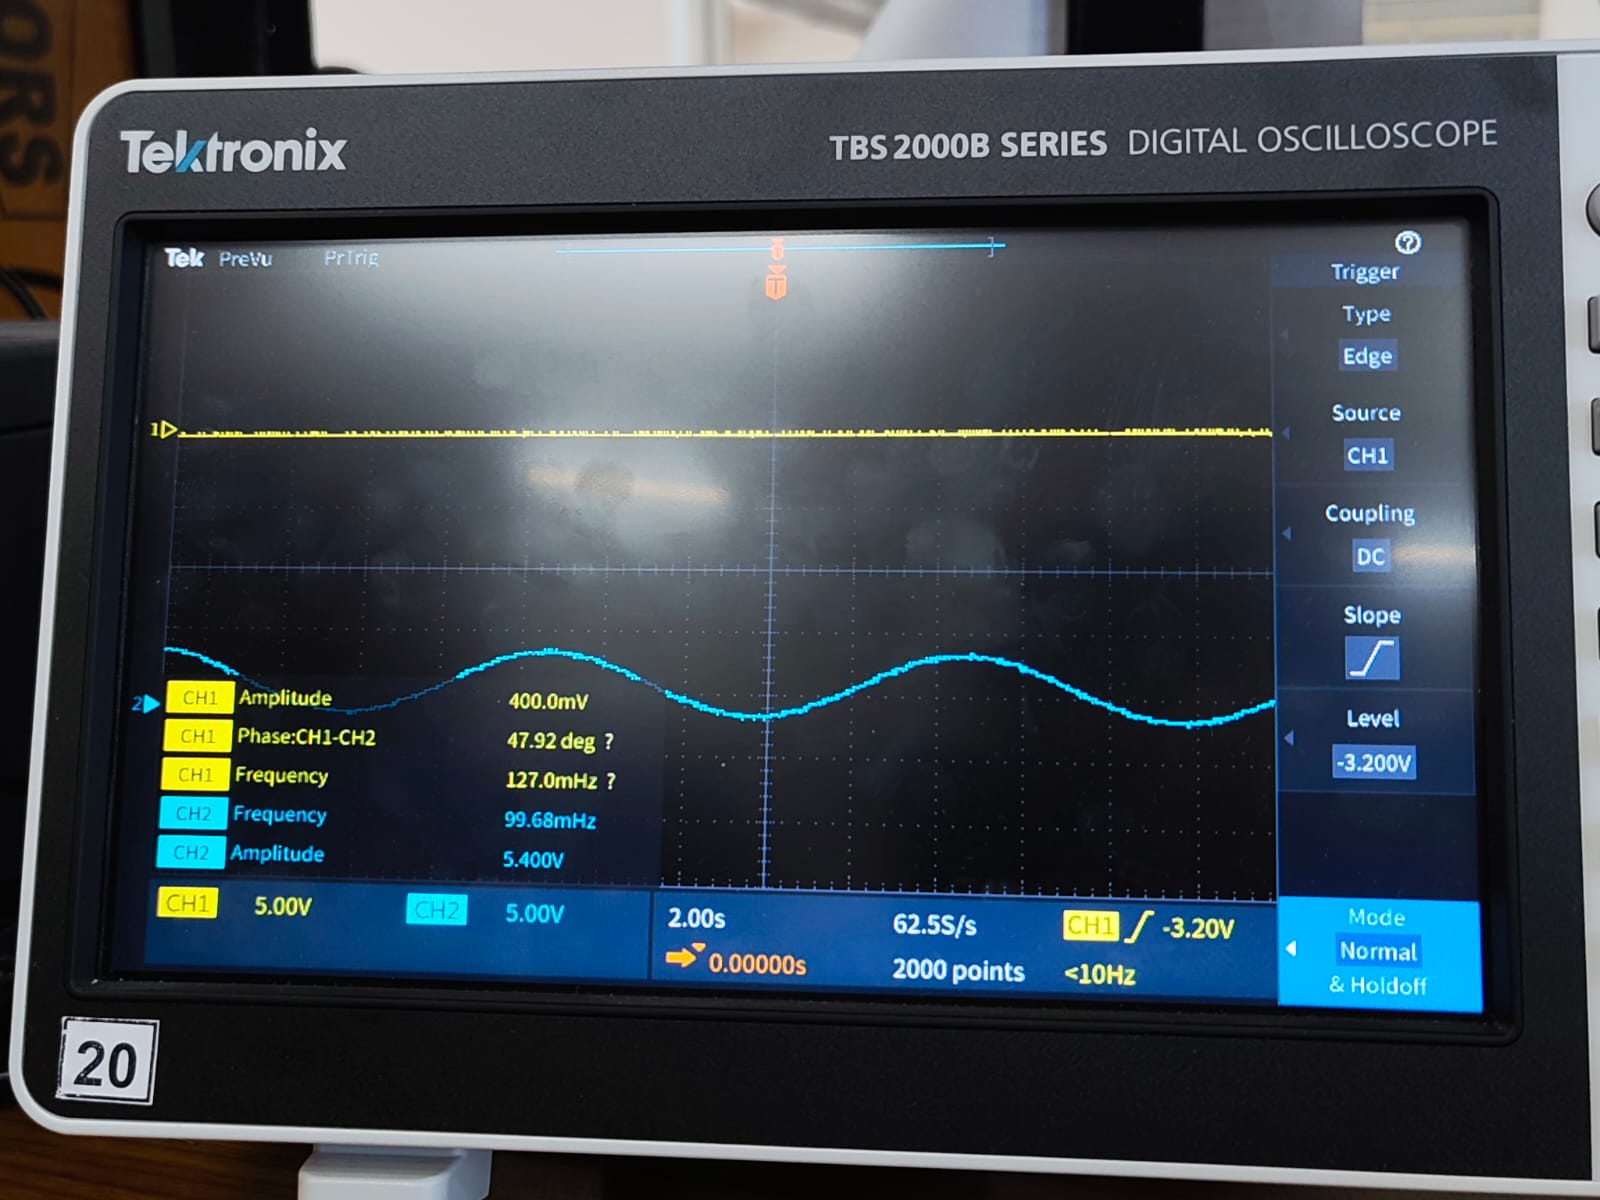
\includegraphics[width=\textwidth]{100mcr.jpeg}
    \caption*{(a) 100mHz}
    \end{subfigure}
%     \hfill
    \begin{subfigure}[b]{0.4\textwidth}
    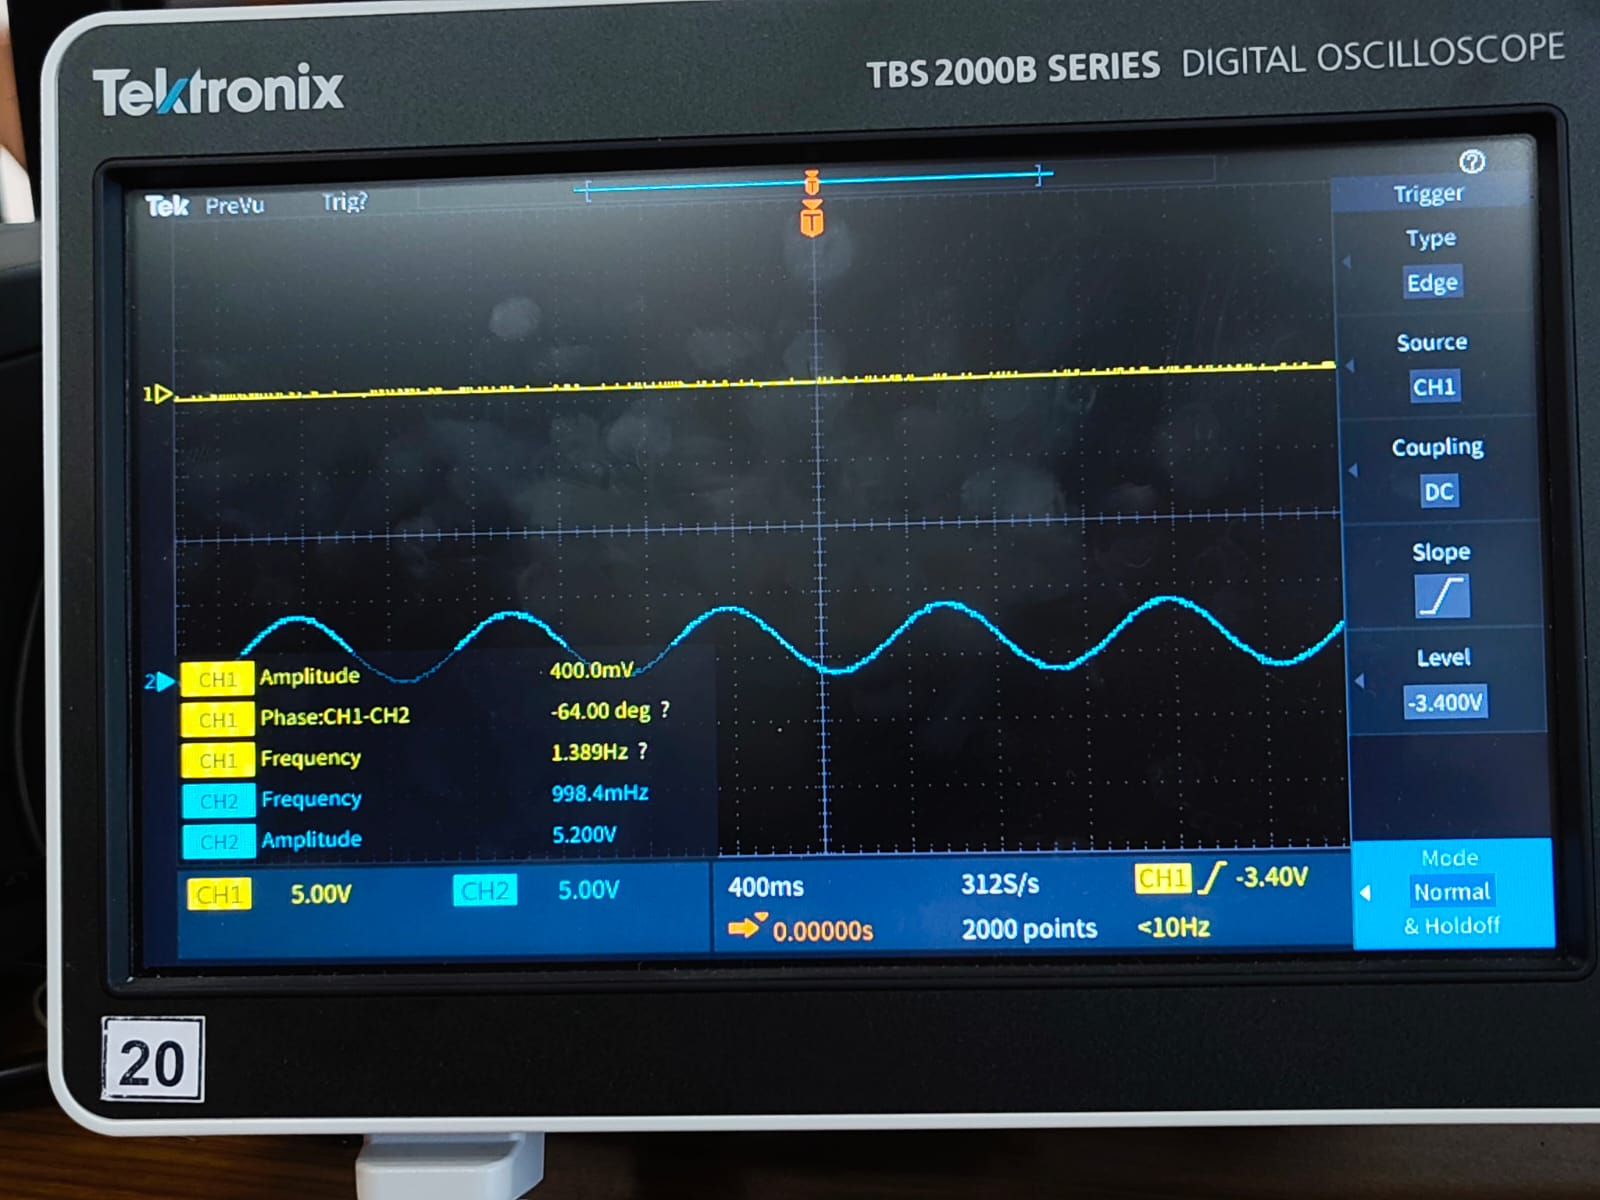
\includegraphics[width=\textwidth]{1cr.jpeg}
    \caption*{(b) 1Hz}
    \centering
    \end{subfigure}
\end{figure}
\vspace{10pt}
\begin{figure}[H]
     \centering
     \begin{subfigure}[b]{0.4\textwidth}
    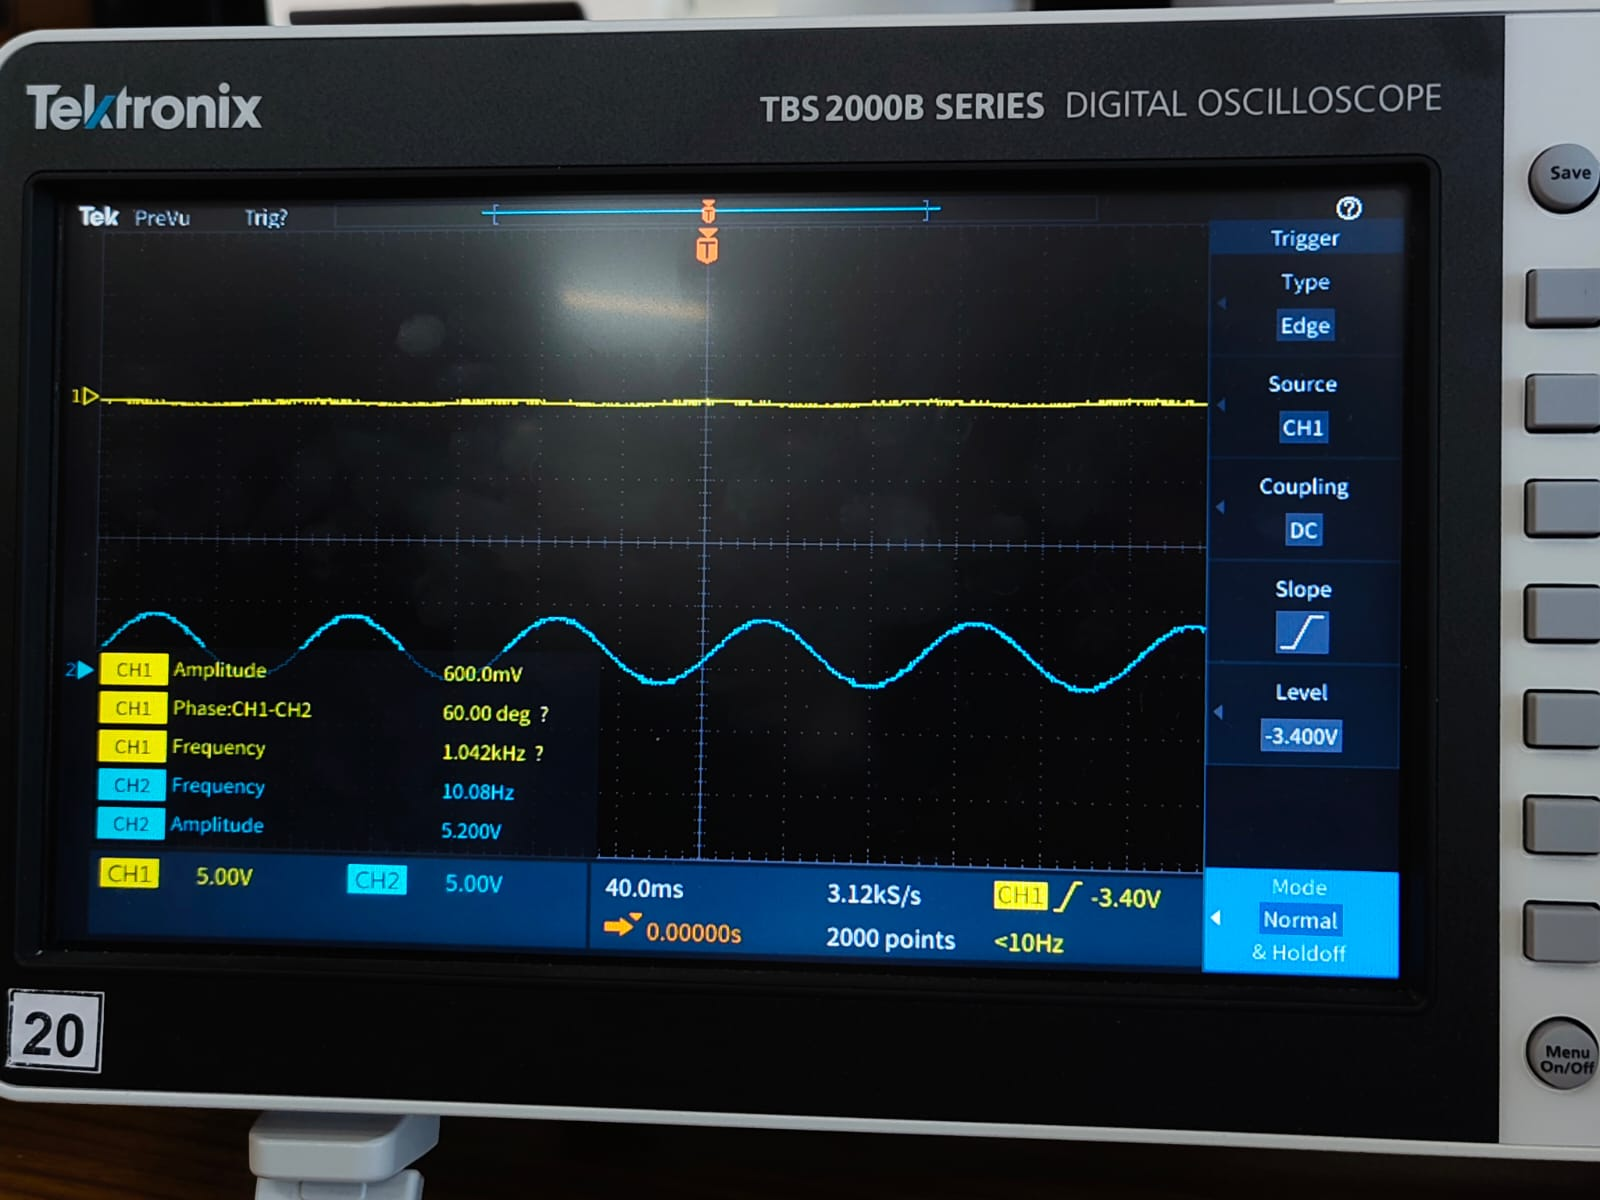
\includegraphics[width=\textwidth]{10cr.jpeg}
    \caption*{(c)10Hz}
    \centering
    \end{subfigure}
 \begin{subfigure}[b]{0.4\textwidth}
    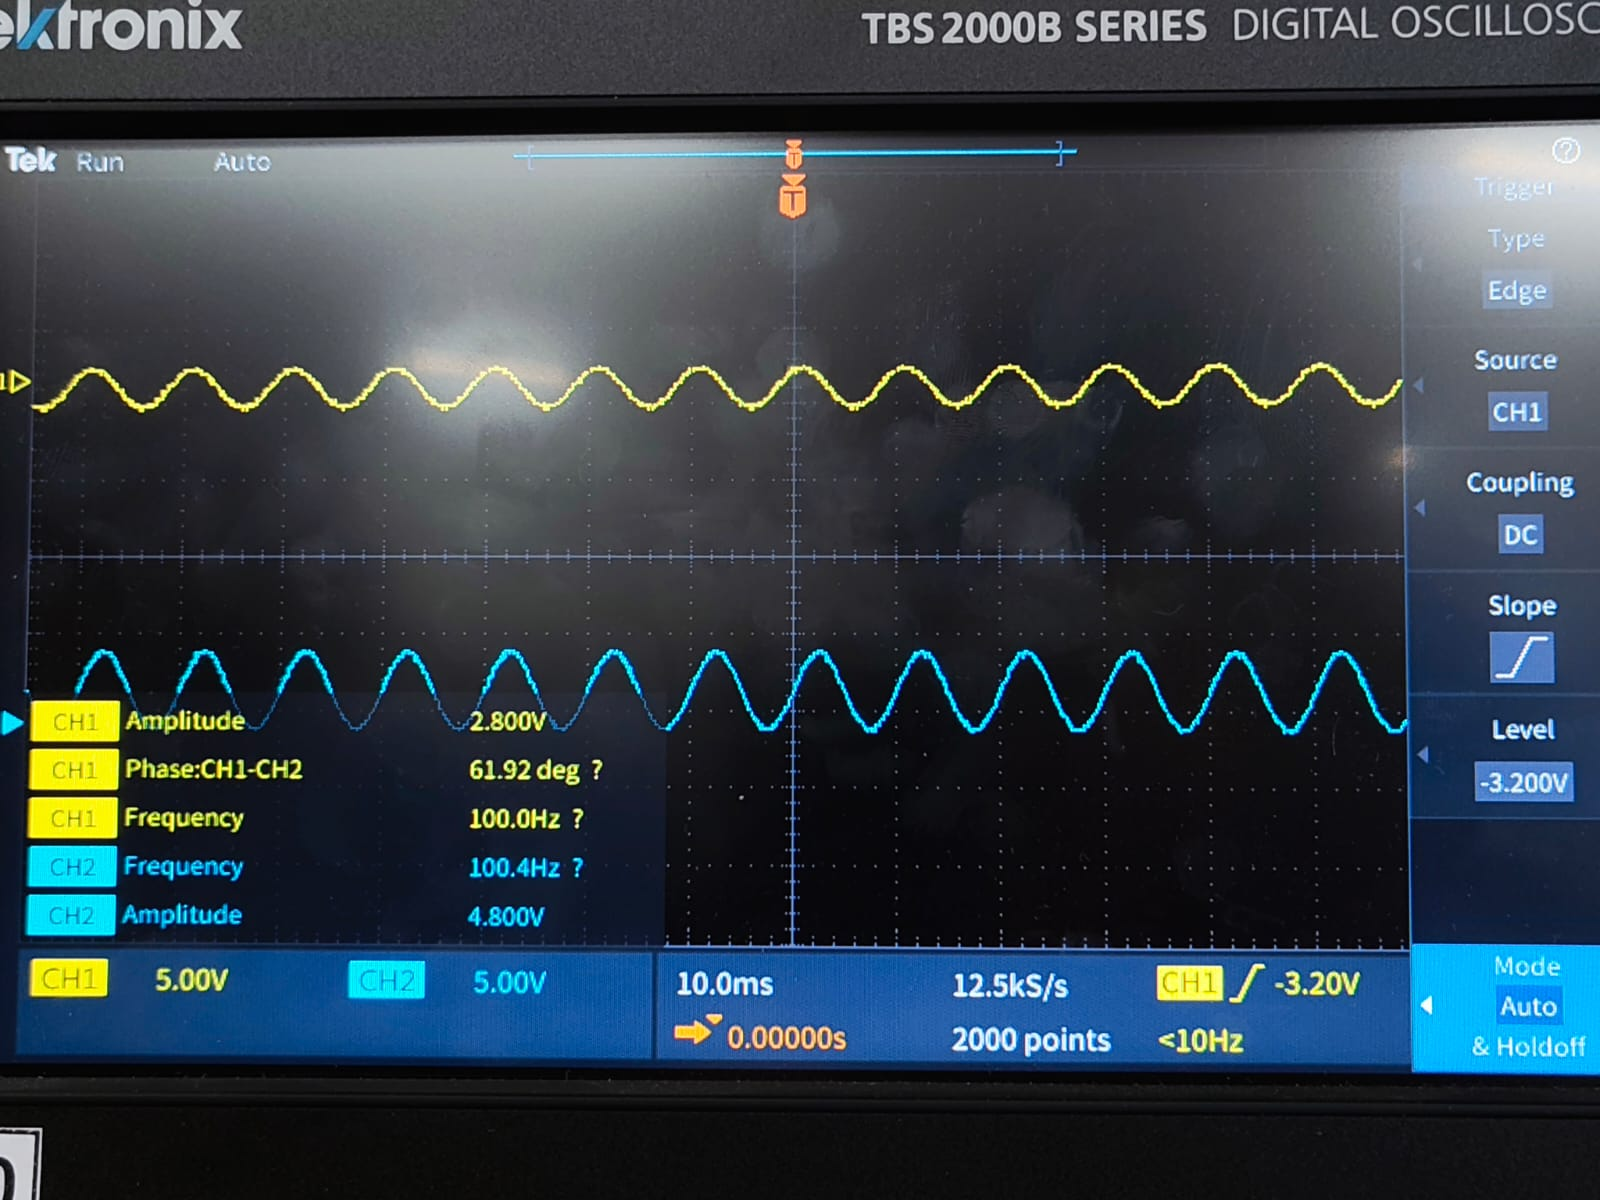
\includegraphics[width=\textwidth]{100cr.jpeg}
    \caption*{(d)100Hz}
    \centering
    \end{subfigure}
\end{figure}  
    \vspace{10pt}

    \begin{figure}[H]
\centering
     \begin{subfigure}[b]{0.4\textwidth}
    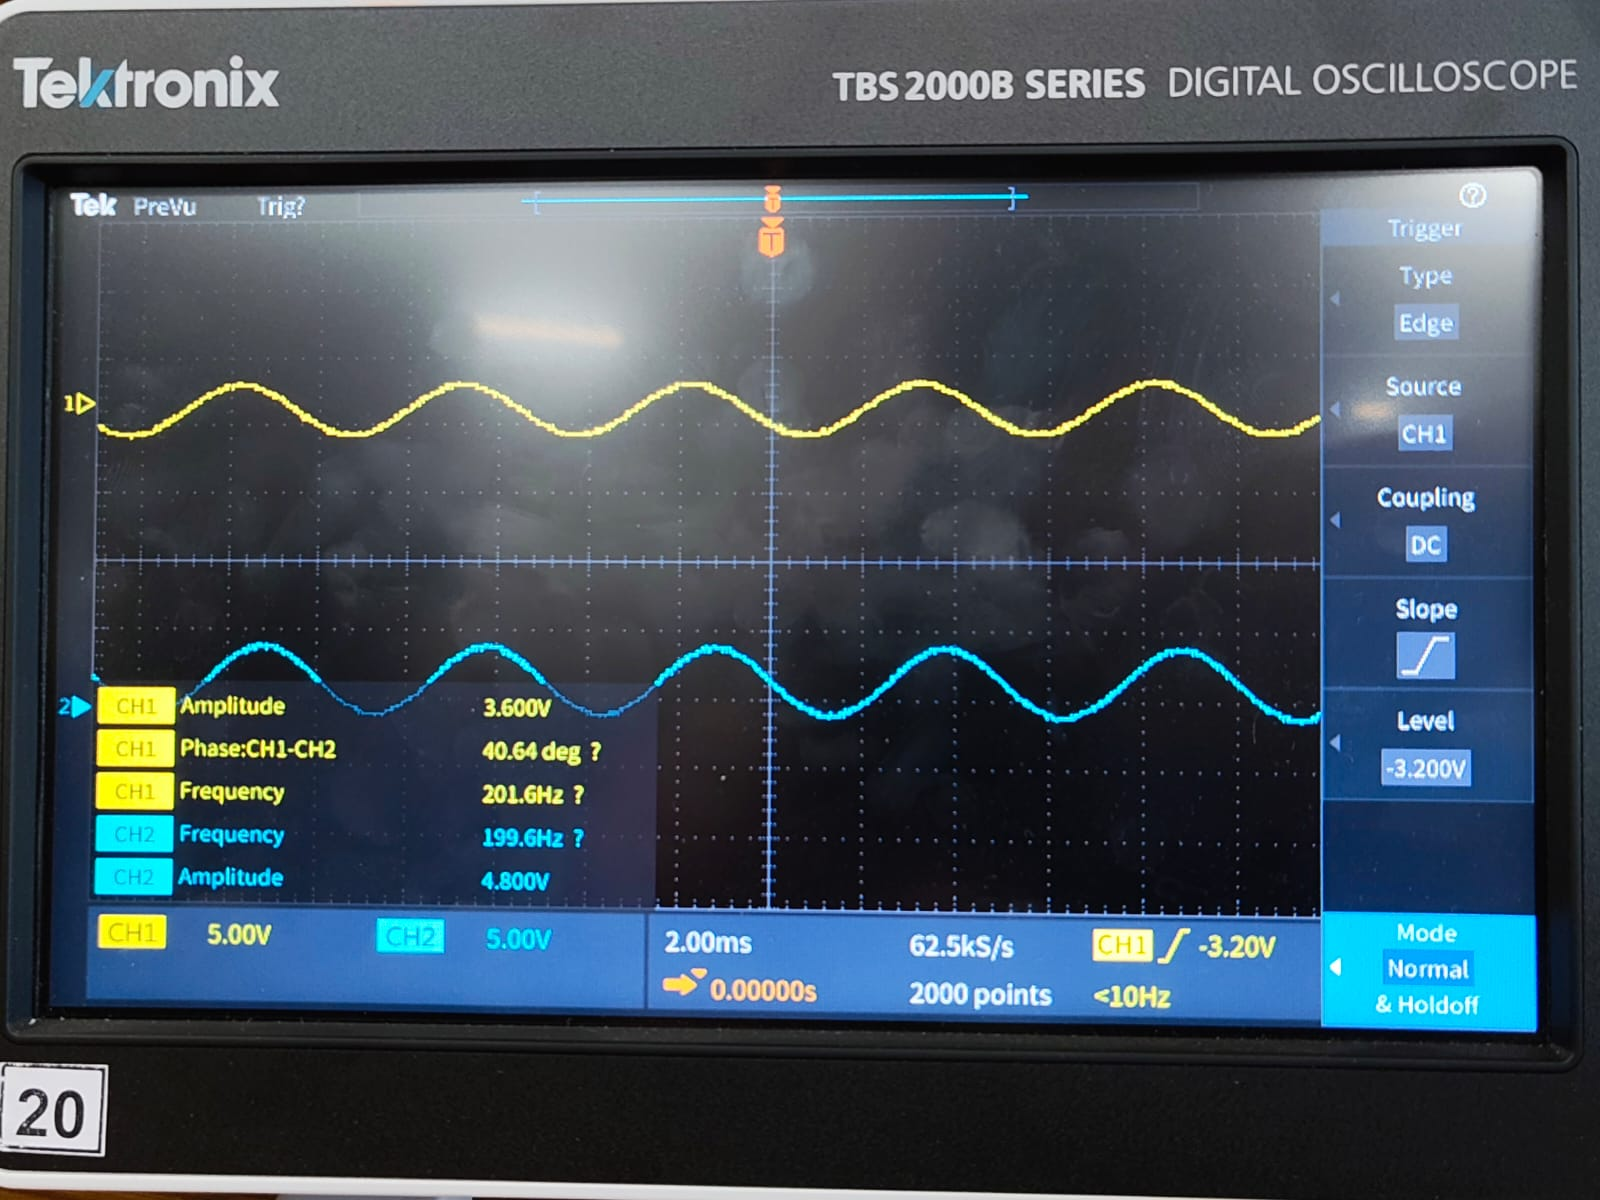
\includegraphics[width=\textwidth]{200cr.jpeg}
    \caption*{(e)200Hz}
    \end{subfigure}
     \begin{subfigure}[b]{0.4\textwidth}
    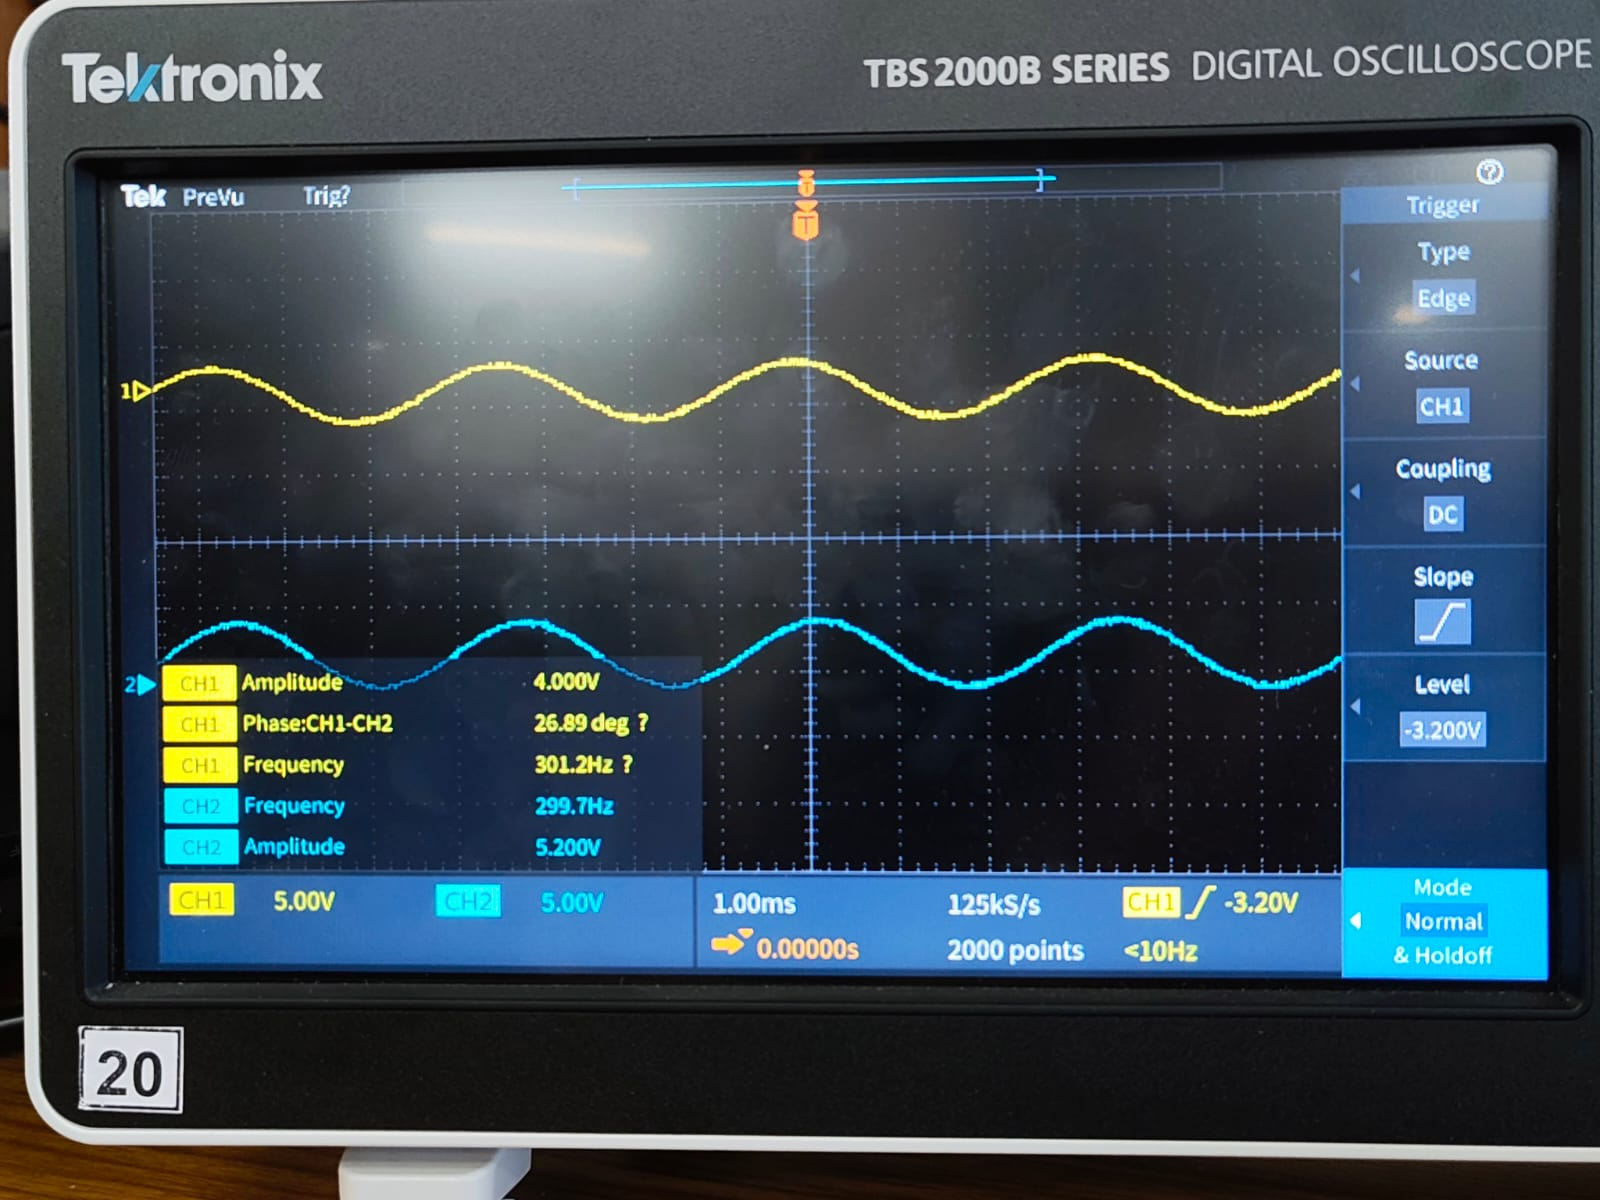
\includegraphics[width=\textwidth]{300cr.jpeg}
    \caption*{(f)300Hz}
    \end{subfigure}
\end{figure}
\vspace{10pt}
\begin{figure}
\centering
     \begin{subfigure}[b]{0.4\textwidth}
    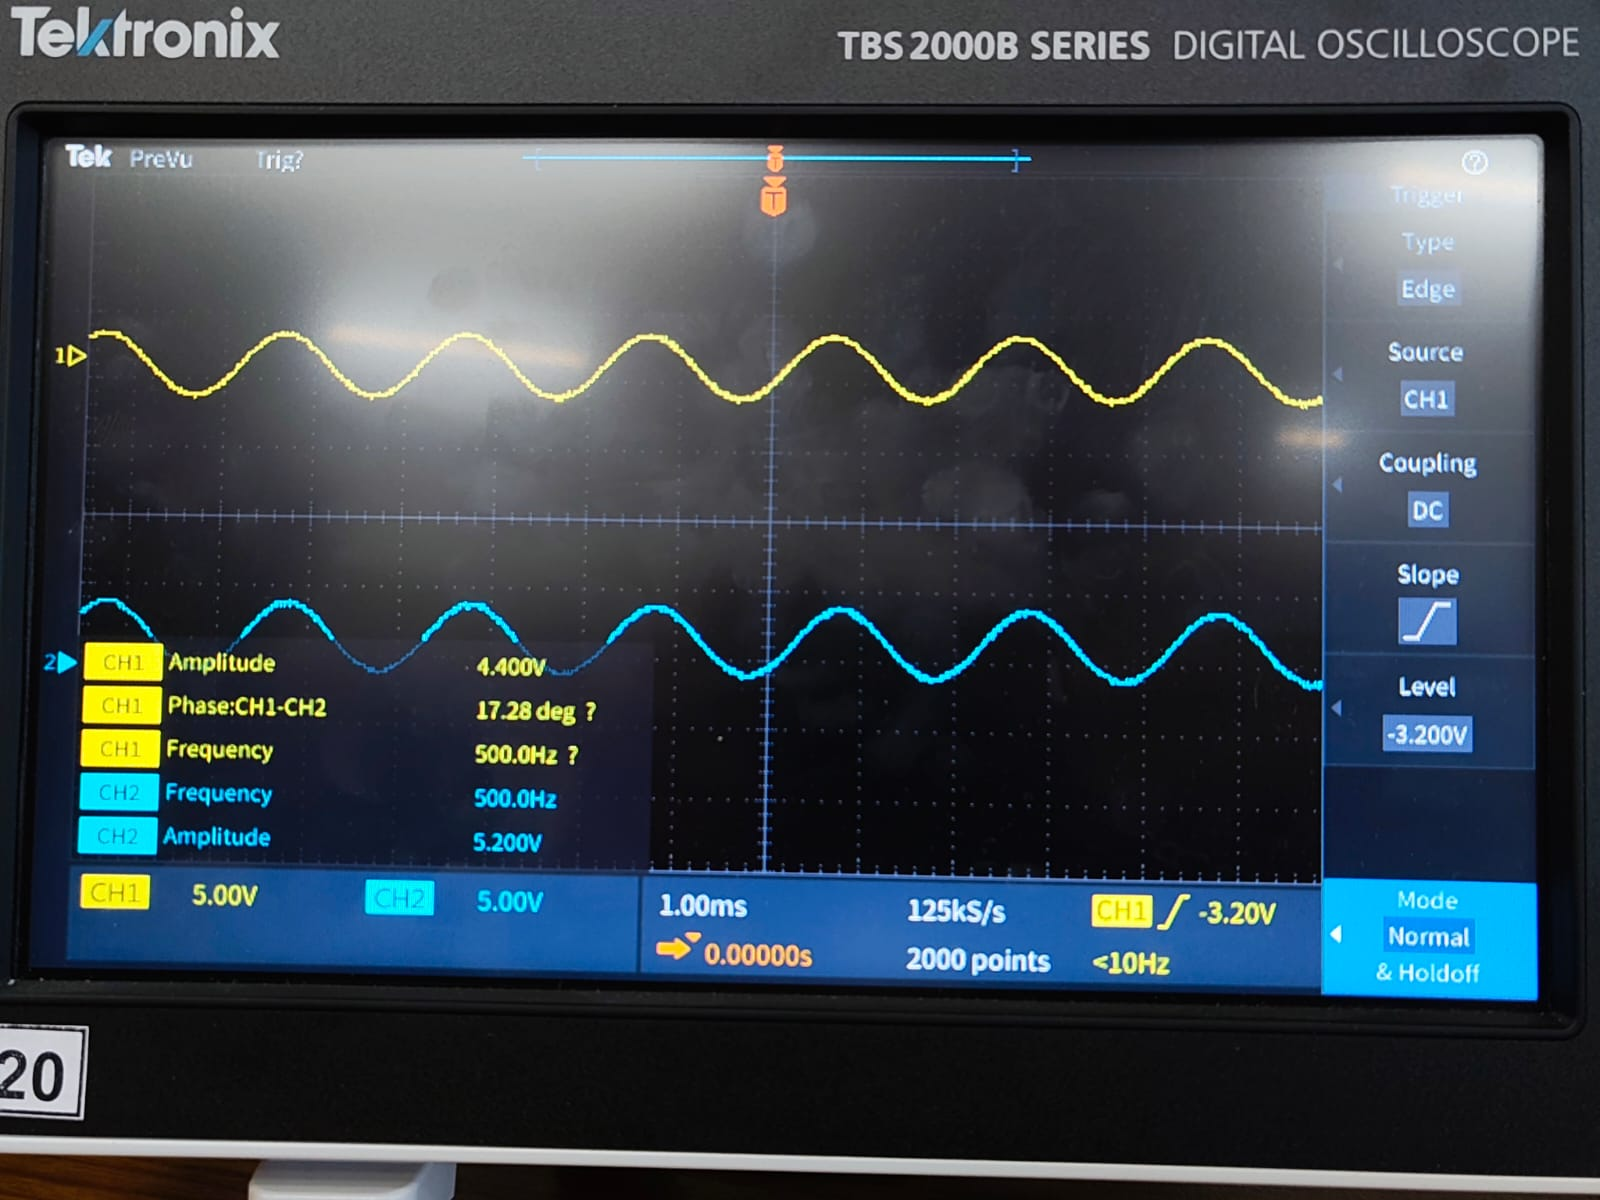
\includegraphics[width=\textwidth]{500cr.jpeg}
    \caption*{(g)500Hz}
    \end{subfigure}
    \begin{subfigure}[b]{0.4\textwidth}
    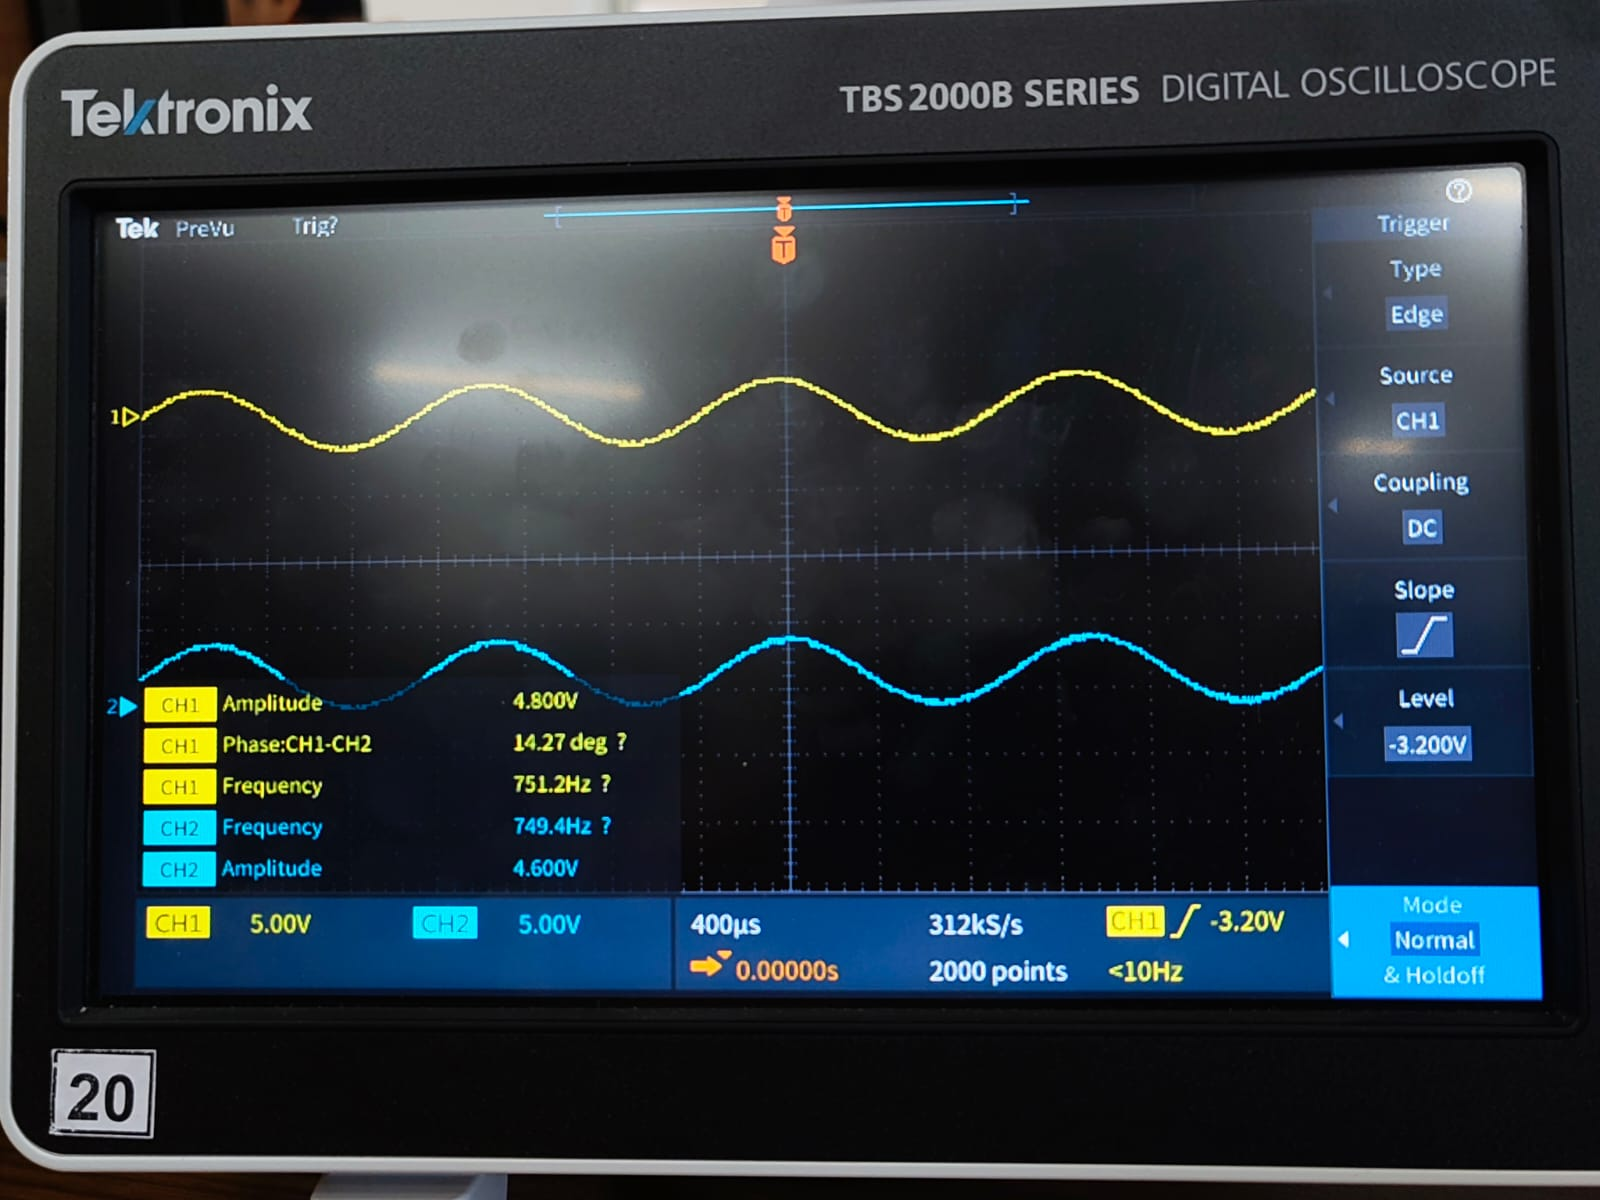
\includegraphics[width=\textwidth]{750cr.jpeg}
    \caption*{(h)750Hz}
    \end{subfigure}
\end{figure}
\vspace{10pt}
\begin{figure}[H]
\centering
     \begin{subfigure}[b]{0.4\textwidth}
    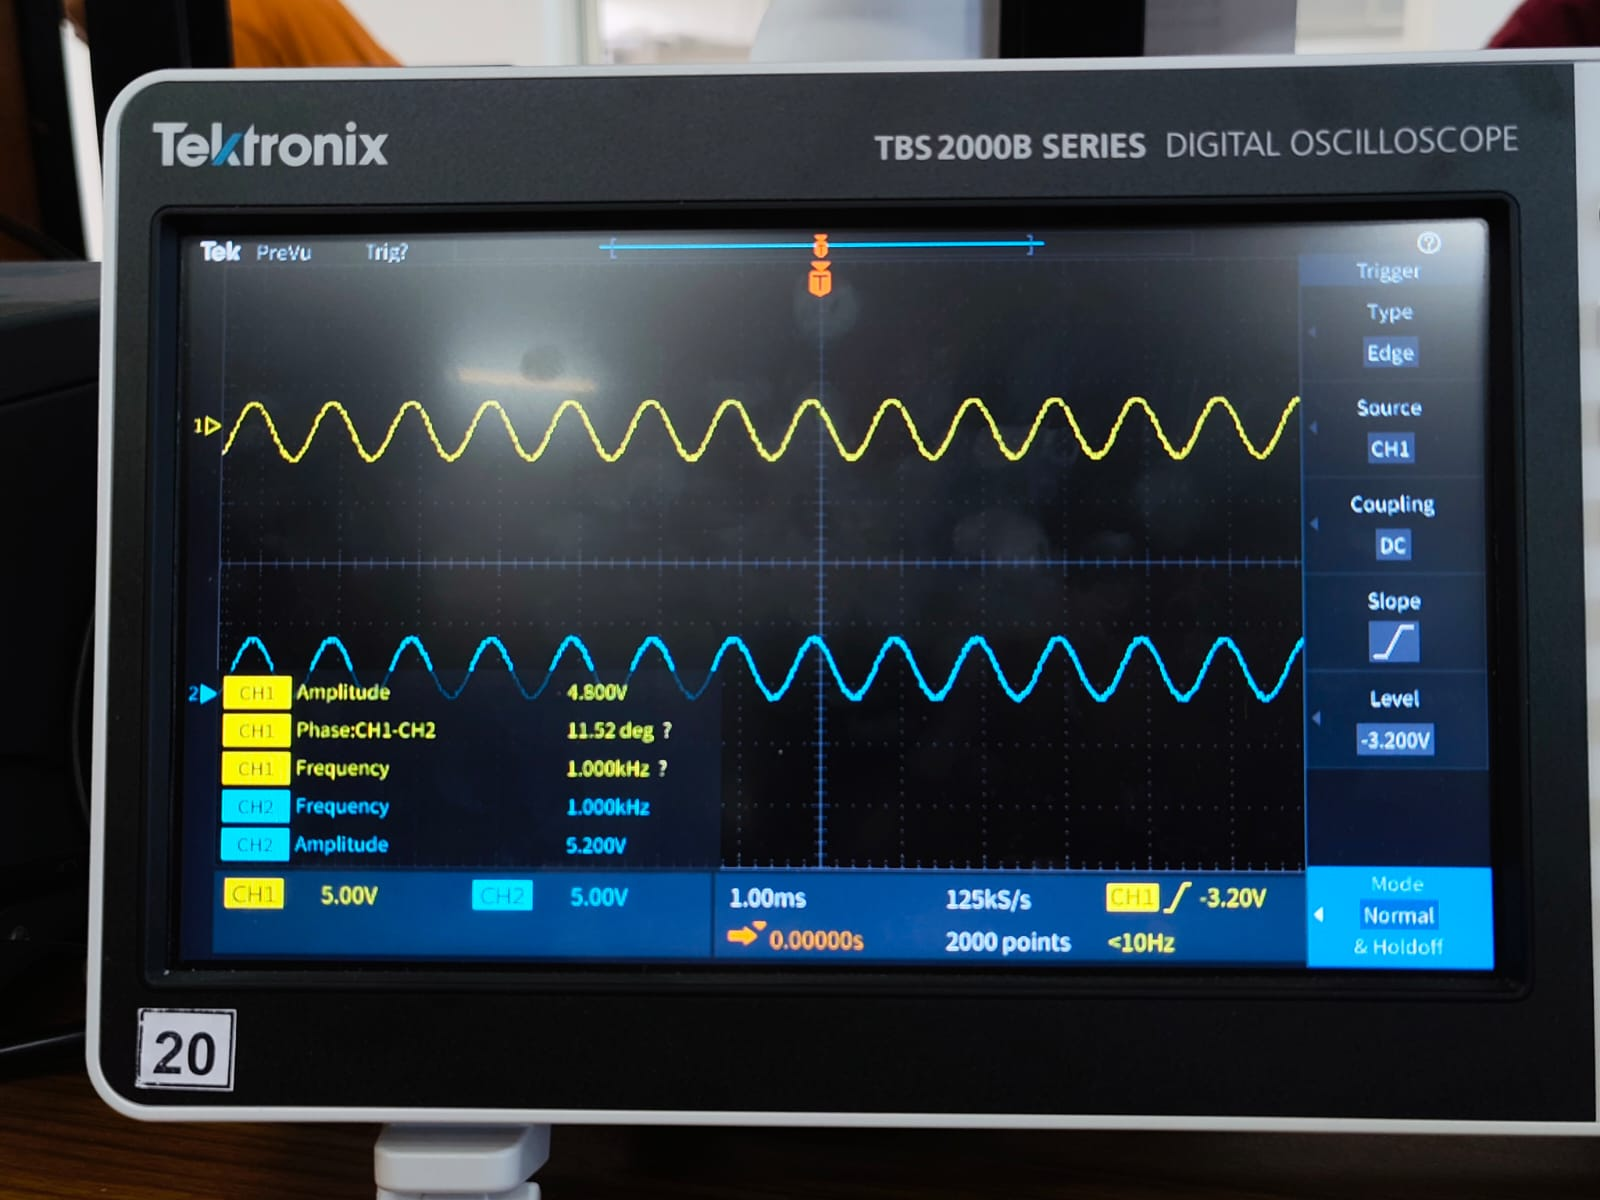
\includegraphics[width=\textwidth]{1kcr.jpeg}
        \caption*{(i)1kHz}
    \end{subfigure}
     \begin{subfigure}[b]{0.4\textwidth}
    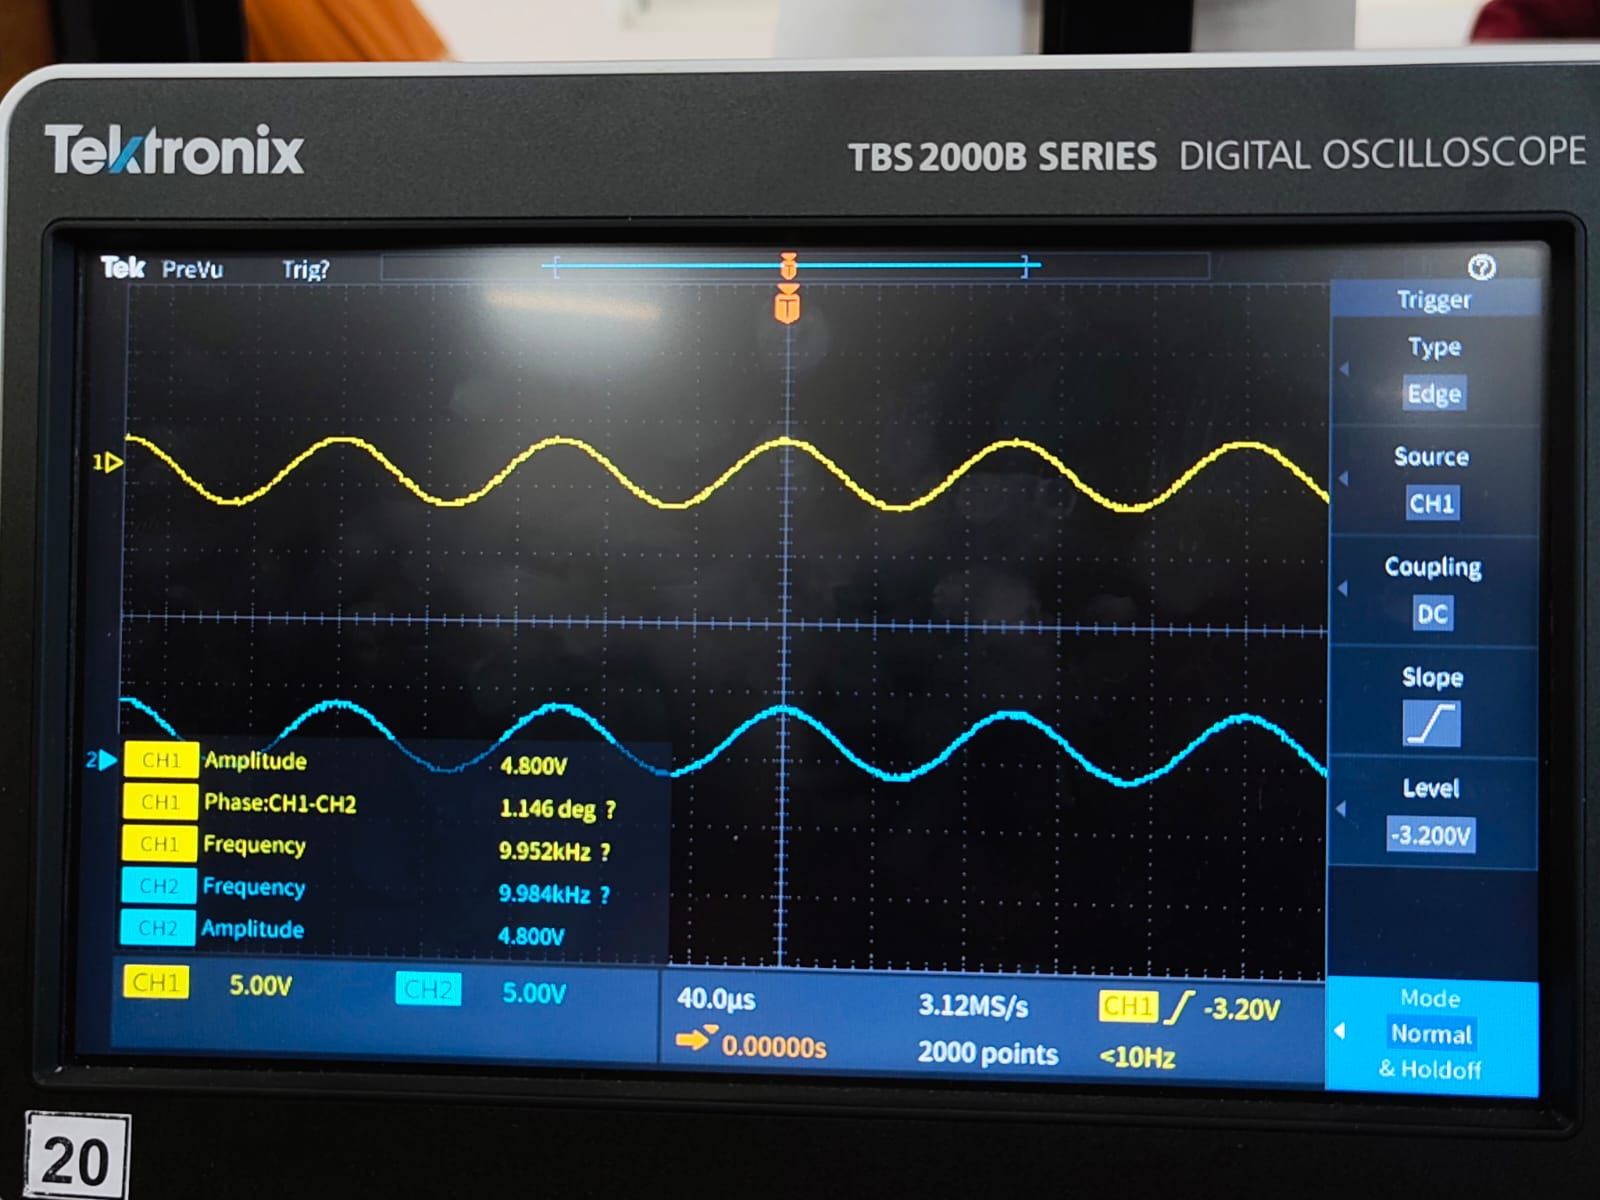
\includegraphics[width=\textwidth]{10kcr.jpeg}
        \caption*{(j)10kHz}
    \end{subfigure}
\end{figure}
\vspace{10pt}
\begin{figure}[H]
\centering
     \begin{subfigure}[h]{0.4\textwidth}
    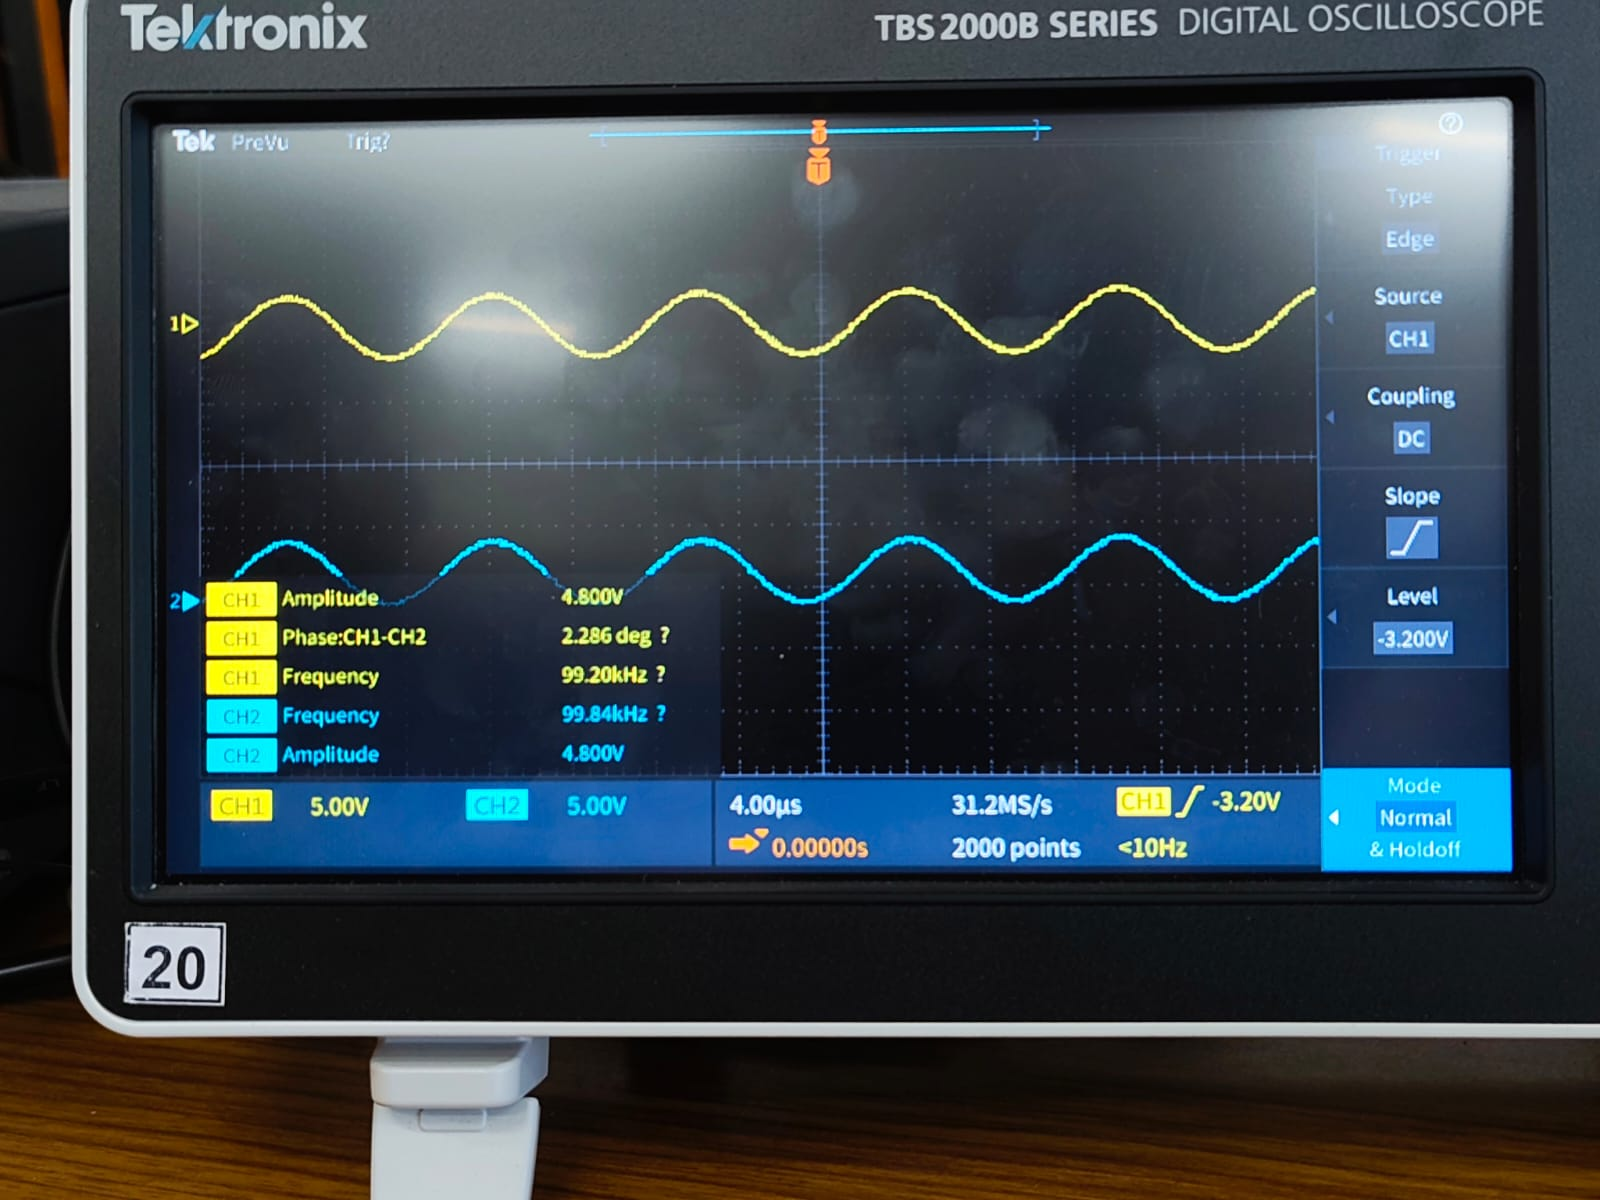
\includegraphics[width=\textwidth]{100kcr.jpeg}
        \caption*{(k)100kHz}
    \end{subfigure}
     \begin{subfigure}[h]{0.4\textwidth}
    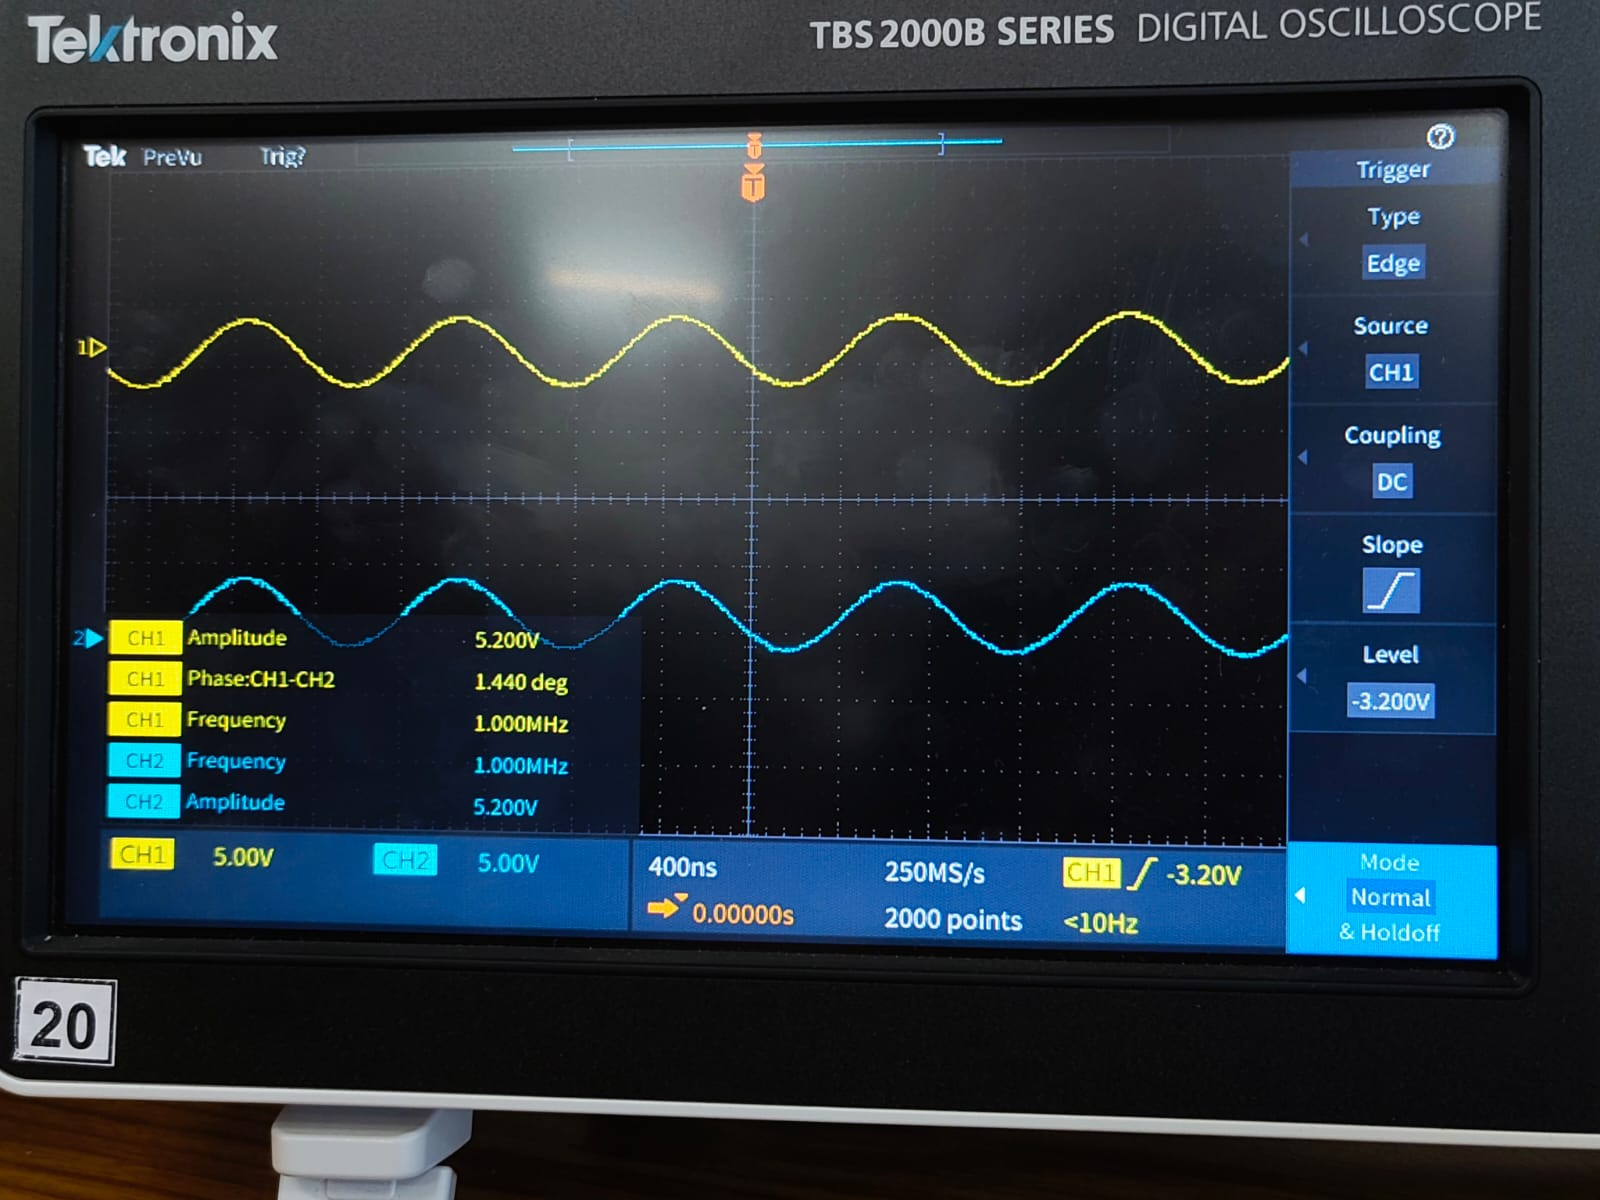
\includegraphics[width=\textwidth]{1Mcr.jpeg}
        \caption*{(l)1MHz}
    \end{subfigure}
    
\end{figure}
\subsection{Simulated Bode Plot}
\begin{figure}[H]
    \centering
    \begin{subfigure}[h]{0.4\textwidth}
    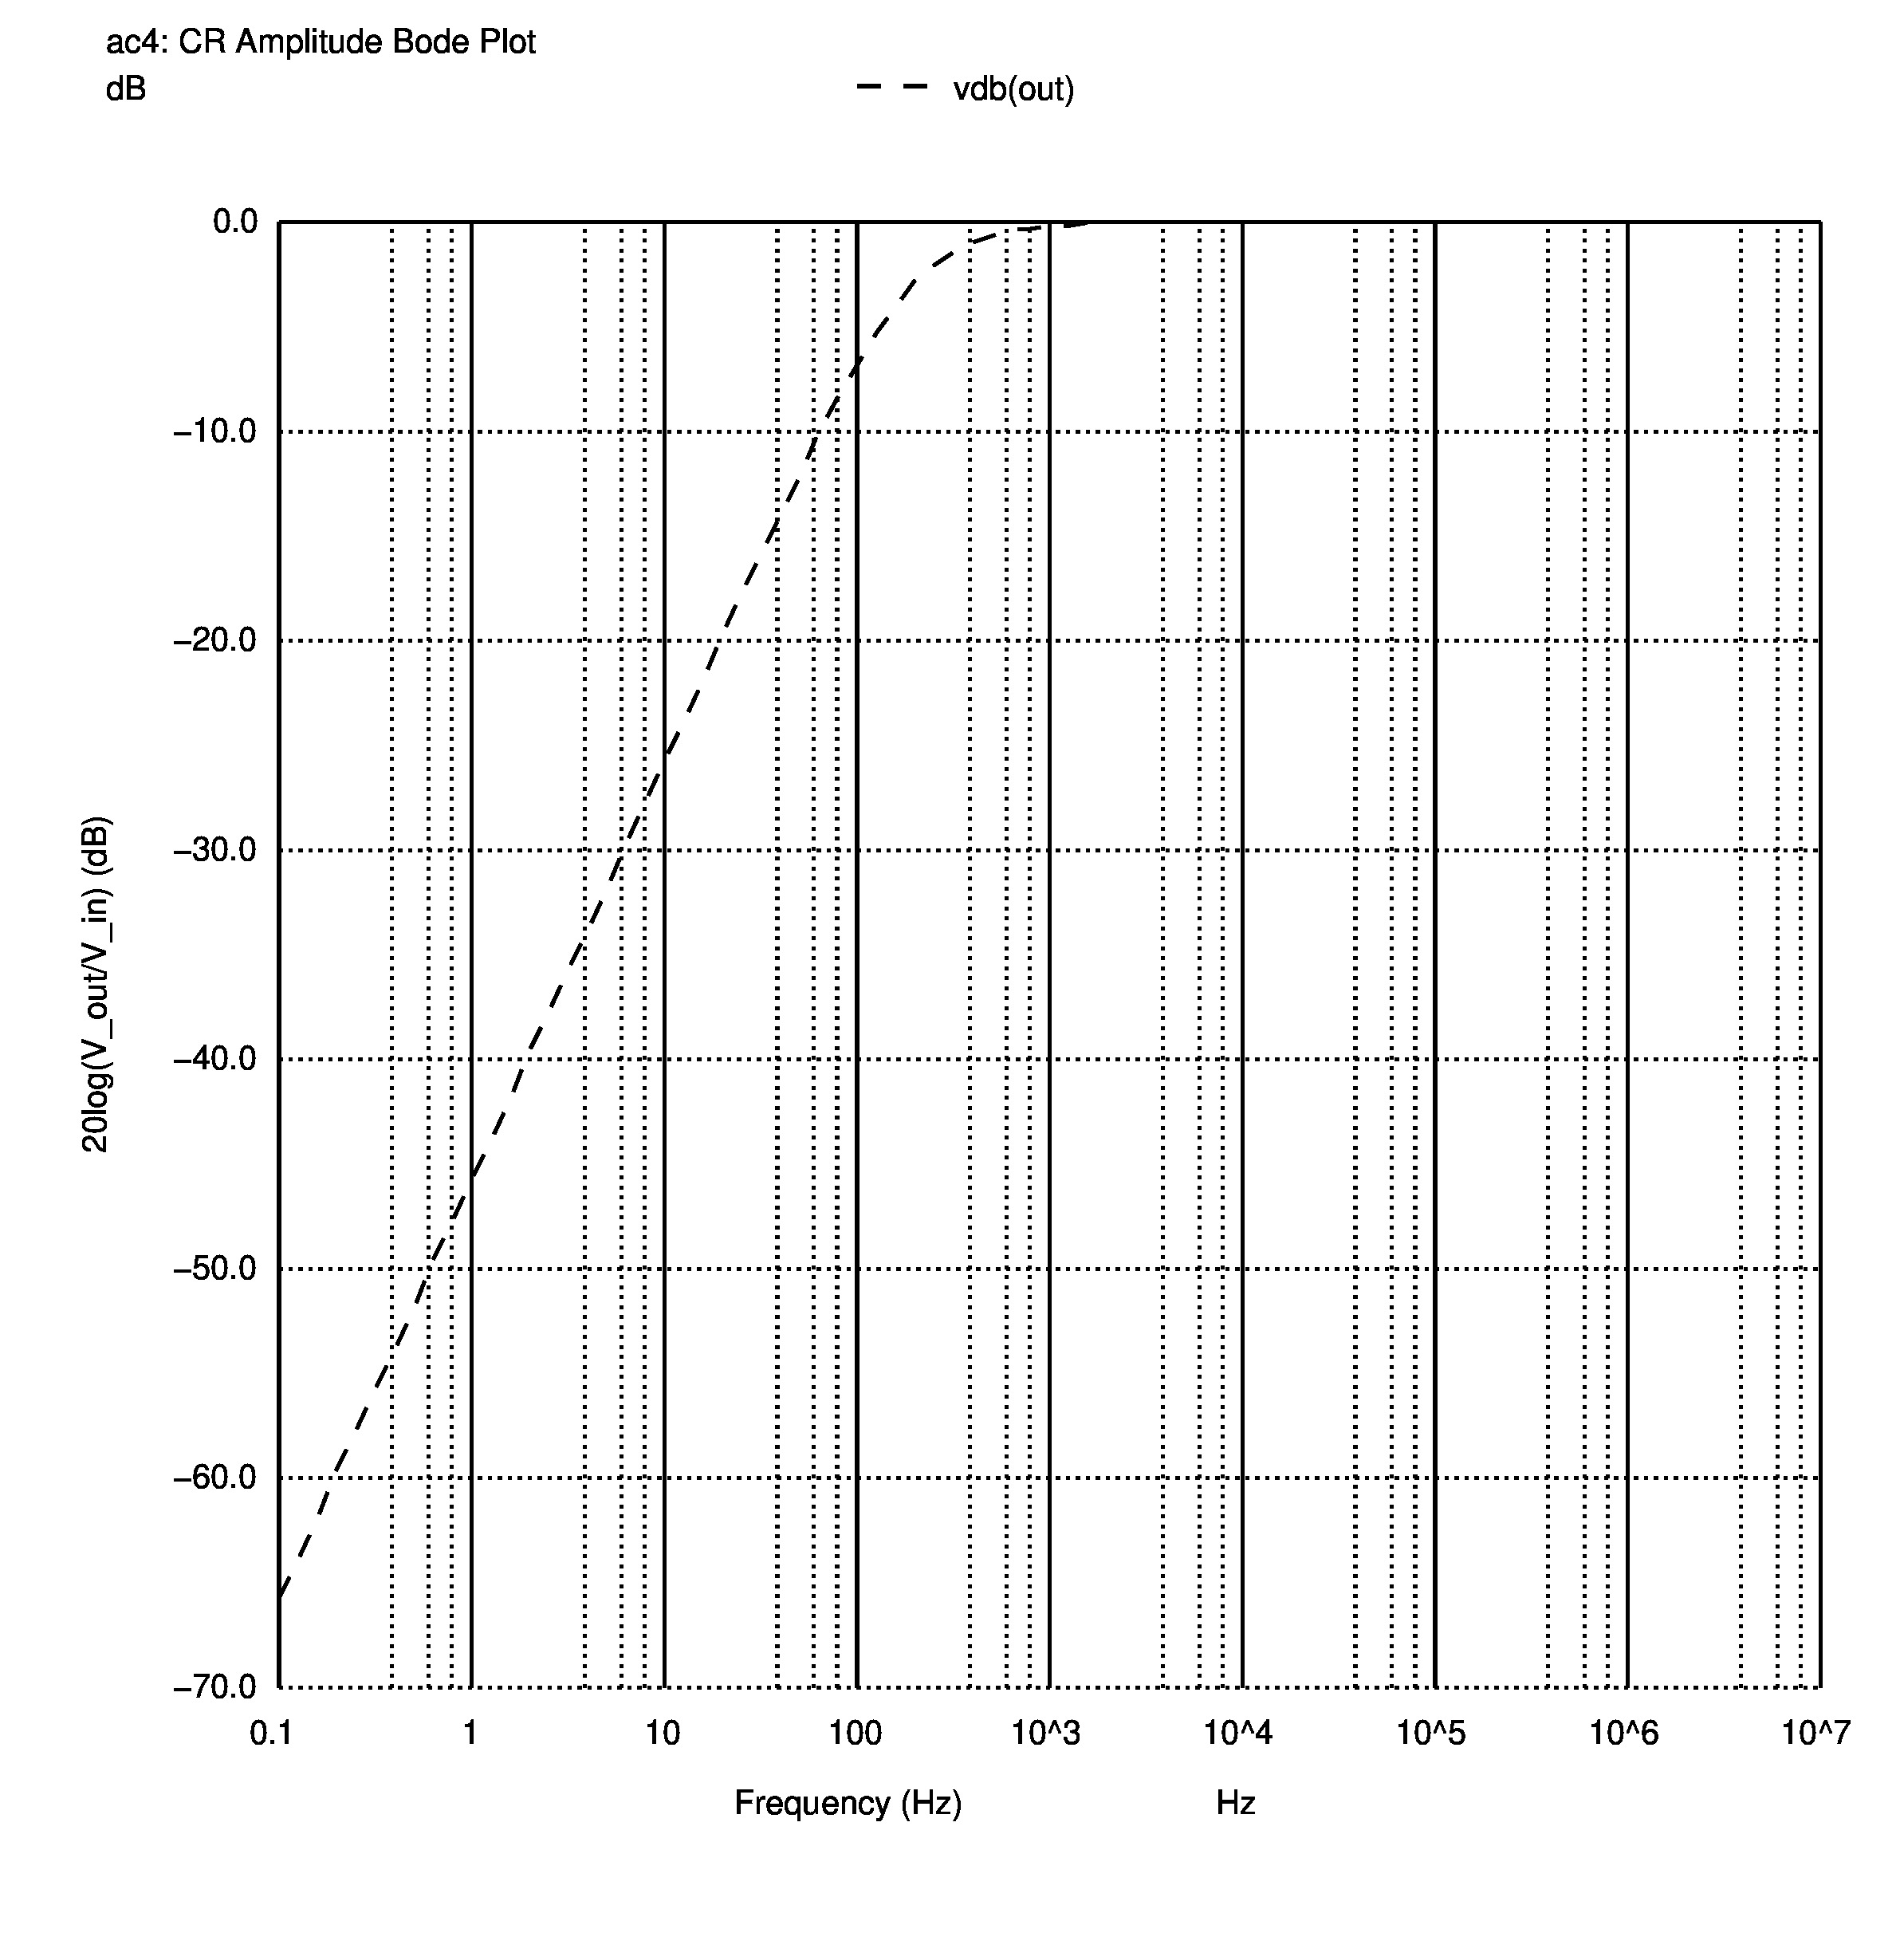
\includegraphics[width=\textwidth]{cr_amp.jpg}
    \caption{Amplitude Bode Plot}
\end{subfigure}
\begin{subfigure}[h]{0.4\textwidth}
    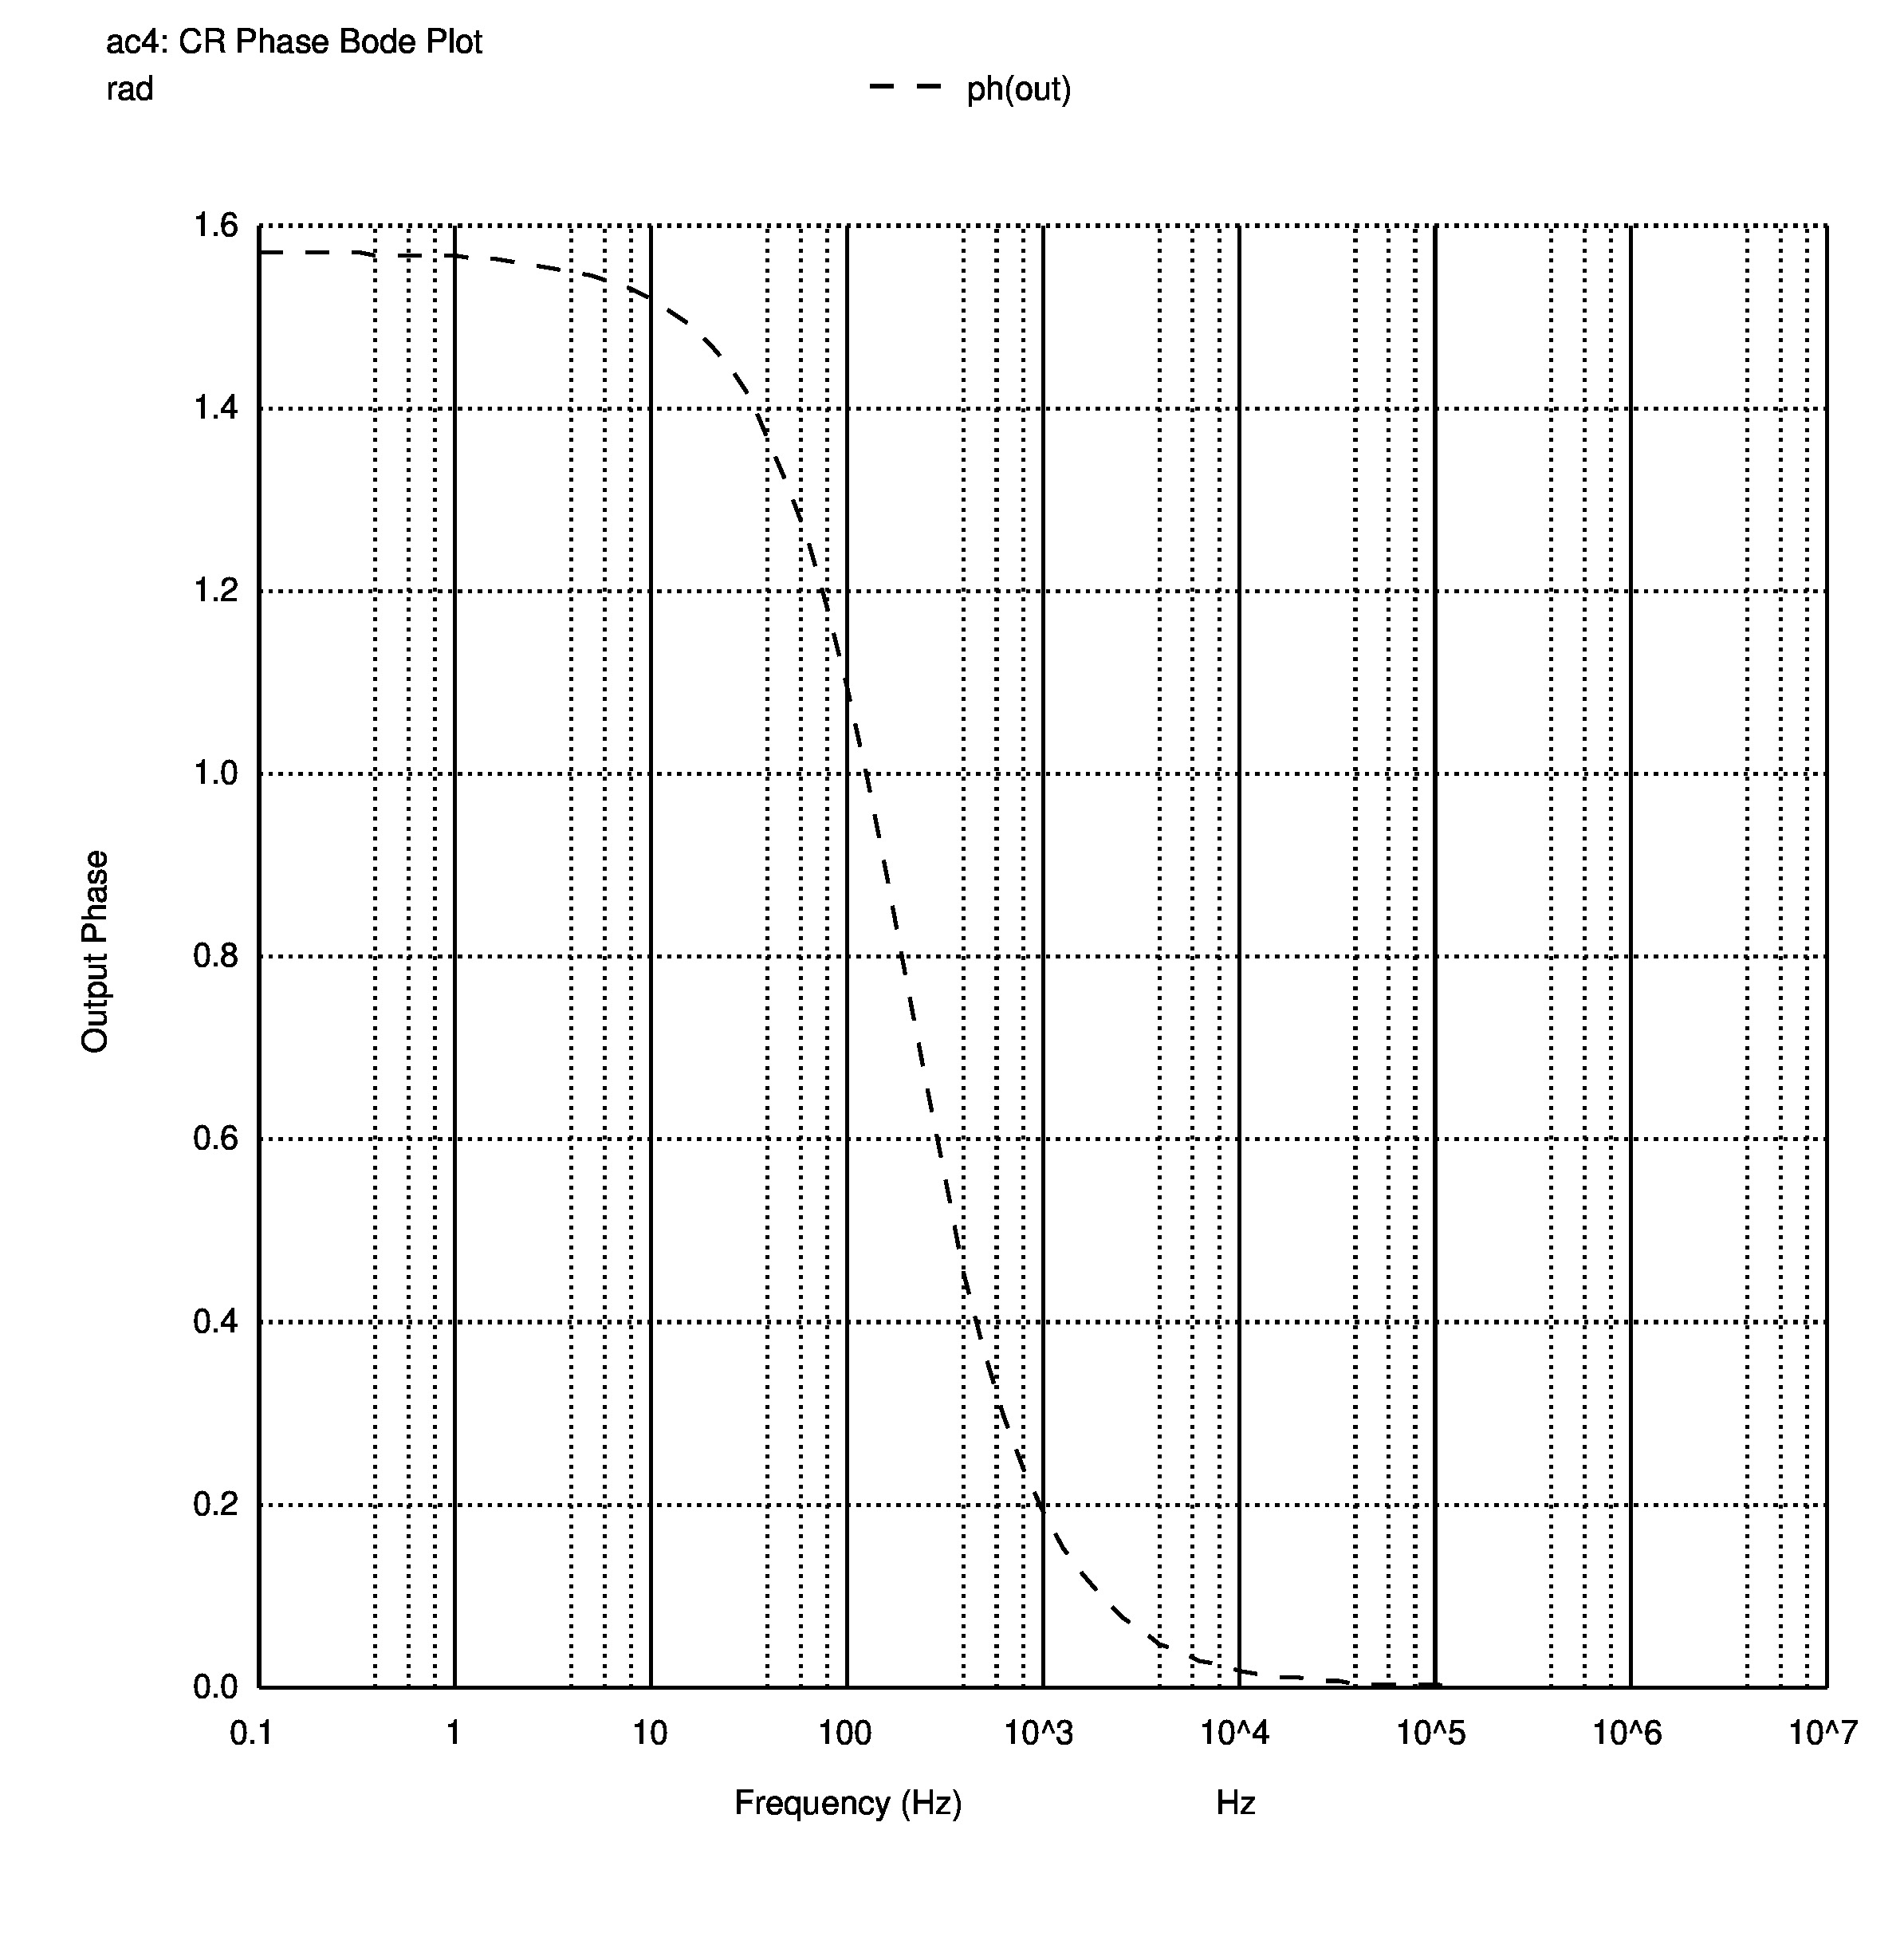
\includegraphics[width=\textwidth]{cr_ph.jpg}
    \caption{Phase Bode Plot}
\end{subfigure}
\end{figure}
\subsection{Manual Bode Plot}
\begin{figure}[H]
    \centering
    \begin{subfigure}[h]{0.4\textwidth}
    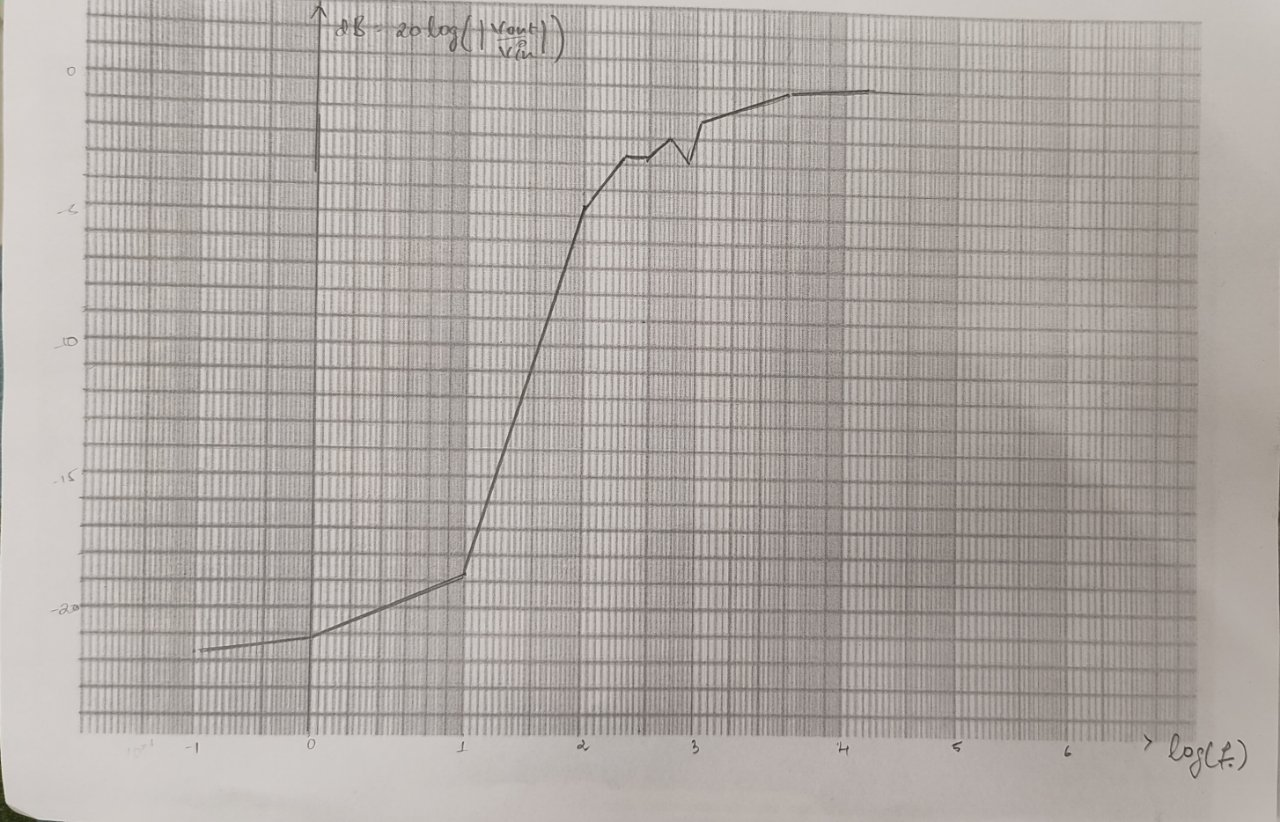
\includegraphics[width=\textwidth]{amp2.jpg}
    \caption{Amplitude Bode Plot}
\end{subfigure}
\end{figure}
\subsection{Results}
\begin{table}[H]
    \centering
    \begin{tabular}{cccc}
        \toprule
        Frequency & Measured $\frac{V_{out}}{V_{in}}$ \\
        \midrule
         $100mHz$ & $0.074$ \\
        $1Hz$ & $0.077$ \\
        $10Hz$ & $0.115$ \\
         $100Hz$ & $0.583$ \\
         $200Hz$ & $0.75$ \\
         $300Hz$ & $0.769$ \\
         $500Hz$ & $0.846$ \\
         $750Hz$ & $0.712$ \\
         $1kHz$ & $0.923$ \\
         $10kHz$ & $1$ \\
         $100kHz$ & $1$ \\
         $1MHz$ & $1$ \\
        \bottomrule
    \end{tabular}
    \caption{Frequency Response for CR}
\end{table}
Thus, we see that the cutoff frequency $\left(=1/2\pi RC\right)$ is 194.1 Hz and the slope of the bode plot is +20dB/decade.

\section{Conclusion}
All our experimental results are nearly accurate and within an error of $5-15\%$ of theoretical results. The simulations have been generated using NGSpice and the code for generating all the simulations are available in our Github repository. The link for the repository is here


\fbox{\parbox{\linewidth}{\url{https://github.com/Vivek-Kumar-1907/ee1200/tree/main/assignment3/simulations/}}}


\end{document}

